        %%******************************************%%
        %%                                          %%
        %%        Modello di tesi di laurea         %%
        %%            di Andrea Giraldin            %%
        %%                                          %%
        %%             2 novembre 2012              %%
        %%                                          %%
        %%******************************************%%

\begin{document}
    \frontmatter
    \begin{titlepage}
    \begin{center}
        \begin{LARGE}
            \textbf{\myUni}\\
        \end{LARGE}

        \vspace{10pt}

        \begin{Large}
            \textsc{\myDepartment}\\
        \end{Large}

        \vspace{10pt}

        \begin{large}
            \textsc{\myFaculty}\\
        \end{large}

        \vspace{30pt}
        \begin{figure}[htbp]
            \centering
            
\includegraphics[height=6cm]{unipd-logo}
        \end{figure}
        \vspace{30pt}

        \begin{LARGE}
            \textbf{\myTitle}\\
        \end{LARGE}

        \vspace{10pt}

        \begin{large}
            \textsl{\myDegree}\\
        \end{large}

        \vspace{40pt}

        \begin{large}
            \begin{flushleft}
                \textit{Relatore}\\
                \vspace{5pt}
                \profTitle\ \myProf
            \end{flushleft}

            % You can tweak the spacing to have professor and student names on the same line
            % useful if the page is broken by a long thesis title and you need more space
            \vspace{-52pt}

            \begin{flushright}
                \textit{Laureando}\\
                \vspace{5pt}
                \myName \\
                \vspace{5pt}
                \textit{Matricola} \myID
            \end{flushright}
        \end{large}

        \vspace{40pt}

        \line(1, 0){338} \\
        \begin{normalsize}
            \textsc{Anno Accademico \myAA}
        \end{normalsize}
    \end{center}
\end{titlepage}

    \clearpage
\phantomsection
\thispagestyle{empty}

\hfill
\vfill

\noindent\myName: \textit{\myTitle,}
\myDegree,
\textcopyright\ \myTime.

    \cleardoublepage
\phantomsection
\pdfbookmark{Sommario}{Sommario}
\begingroup
\let\clearpage\relax
\let\cleardoublepage\relax
\let\cleardoublepage\relax

\chapter*{Sommario}

Il presente documento descrive il lavoro svolto durante il periodo di stage dal laureando
Valerio Occhinegro presso l’azienda Spazio Dev Srl di Tombolo (PD). Lo stage, svoltosi al termine del percorso di studi della Laurea Triennale in "Scienze Informatiche", ha avuto una durata complessiva di 306 ore.

Il lavoro in questione è stato suddiviso in 4 diverse fasi, ognuna delle quali caratterizzata da obiettivi specifici e scadenze precise, e si basa su un'analisi intelligente di siti web, improntata alla vendita dei servizi aziendali a potenziali clienti. Il ruolo del laureando è quello di gestire e archiviare i siti web target e successivamente classificarli per fornire a Spazio Dev input utili per acquisire l'abilità di ampliare la quantità dei propri clienti in maniera rapida e automatizzata. 
Nello specifico, il progetto di stage ha l’obiettivo di sviluppare competenze avanzate nell’intelligenza artificiale, con un focus
particolare sulla classificazione e organizzazione dei dati; uno studio che si inserisce nel contesto di
{“SalesCRM: Customer Relationship Manager ”, un sistema integrato che mira a ottimizzare la gestione delle relazioni con i clienti e a migliorare l’efficienza dei venditori.} INSERIRE VERO TITOLO
Lo scopo ultimo del progetto è la creazione di un sistema intelligente che sia in grado di analizzare dataset complessi,
classificare la qualità dei siti web (siti che potrebbero essere migliorati e siti che non necessitano di modifiche) e proporre i propri servizi alle aziende che ne necessitano in maniera automatica. 
Il laureando è responsabile dello sviluppo di funzionalità chiave del sistema che consentiranno di fornire
soluzioni strategiche agli utilizzatori della piattaforma. 



%\vfill

%\selectlanguage{english}
%\pdfbookmark{Abstract}{Abstract}
%\chapter*{Abstract}

%\selectlanguage{italian}

\endgroup

\vfill

    \cleardoublepage
\phantomsection
\pdfbookmark{Ringraziamenti}{ringraziamenti}

\begin{flushright}{
    \slshape
    ``Non importa quanto piano vai, finché non ti fermi''} \\
    \medskip
    --- Confucio
\end{flushright}


\bigskip

\begingroup
\let\clearpage\relax
\let\cleardoublepage\relax
\let\cleardoublepage\relax

\chapter*{Ringraziamenti}

\noindent \textit{
    Prima di tutto vorrei ringraziare profondamente il Prof. \myProf, per avermi aiutato durante la stesura di questa tesi; senza i suoi consigli e la sua disponibilità fuori dal comune avrei sicuramente scritto un elaborato di qualità inferiore. Ha svolto un lavoro talmente impeccabile da meritarsi tutta la mia stima e per quel poco che conta un po'di pubblicità positiva con i miei colleghi che devono ancora laurearsi.
    }\\

\noindent \textit{
    Ringrazio tutta la mia famiglia, i miei zii e i miei cugini per essermi stati vicini e avermi sostenuto in questi anni difficili.
    }\\

\noindent \textit{
    Dedico degli ulteriori ringraziamenti ai miei amici Irene, Paño, Alessia e Mattia che mi hanno aiutato a tenere alto il morale durante questo percorso; a tutti i colleghi universitari il cui supporto è stato di fondamentale importanza per superare gli ultimi esami e all'intero Dipartimento di Chimica per avermi ospitato innumerevoli volte.  
    }\\

\noindent \textit{
    Un ringraziamento particolare è riservato a Matteo che posso considerare un vero e proprio fratello maggiore (senza nulla da togliere a Claudia), lo ringrazio per avermi aiutato durante uno degli anni più faticosi e per avermi fatto appassionare al mondo della "Geomatica".
    }\\
\bigskip

\noindent\textit{\myLocation, \myTime}
\hfill \myName

\endgroup

    \cleardoublepage
\pdfbookmark{\contentsname}{tableofcontents}
\setcounter{tocdepth}{2}
\tableofcontents
%\markboth{\contentsname}{\contentsname}
\clearpage

\begingroup
    \let\clearpage\relax
    \let\cleardoublepage\relax
    \let\cleardoublepage\relax

    % Figures list
    \phantomsection
    \pdfbookmark{\listfigurename}{lof}
    \listoffigures

    \vspace*{8ex}

    \newpage
    % Tables list
    \phantomsection
    \pdfbookmark{\listtablename}{lot}
    \listoftables

    \vspace*{8ex}
\endgroup

\cleardoublepage

    \cleardoublepage

    \mainmatter
    \chapter{Introduzione}
\label{cap:introduzione}

Introduzione al contesto applicativo.\\

\noindent Esempio di utilizzo di un termine nel glossario \\
\gls{api}. \\

\noindent Esempio di citazione in linea \\
\cite{site:agile-manifesto}. \\

\noindent Esempio di citazione nel pie' di pagina \\
citazione\footcite{womak:lean-thinking} \\

\section{L'azienda}

Descrizione dell'azienda.

\section{L'idea}

Introduzione all'idea dello stage.

\section{Organizzazione del testo}

\begin{description}
    \item[{\hyperref[cap:processi-metodologie]{Il secondo capitolo}}] descrive ...
    
    \item[{\hyperref[cap:descrizione-stage]{Il terzo capitolo}}] approfondisce ...
    
    \item[{\hyperref[cap:analisi-requisiti]{Il quarto capitolo}}] approfondisce ...
    
    \item[{\hyperref[cap:progettazione-codifica]{Il quinto capitolo}}] approfondisce ...
    
    \item[{\hyperref[cap:verifica-validazione]{Il sesto capitolo}}] approfondisce ...
    
    \item[{\hyperref[cap:conclusioni]{Nel settimo capitolo}}] descrive ...
\end{description}

Riguardo la stesura del testo, relativamente al documento sono state adottate le seguenti convenzioni tipografiche:
\begin{itemize}
	\item gli acronimi, le abbreviazioni e i termini ambigui o di uso non comune menzionati vengono definiti nel glossario, situato alla fine del presente documento;
	\item per la prima occorrenza dei termini riportati nel glossario viene utilizzata la seguente nomenclatura: \emph{parola}\glsfirstoccur;
	\item i termini in lingua straniera o facenti parti del gergo tecnico sono evidenziati con il carattere \emph{corsivo}.
\end{itemize}

    \chapter{Processi e metodologie}
\label{cap:processi-metodologie}

In questo capitolo sono riassunti i processi e le metodologie che lo studente ha applicato durante lo sviluppo del progetto di stage. 

\section{Gestione della configurazione}
La gestione della configurazione è il processo tramite il quale è possibile identificare, controllare e coordinare i vari componenti del software e le risorse ad esso associate durante l'intero ciclo di vita del prodotto. Grazie a questo processo gli sviluppatori possono tenere traccia delle modifiche e gestire le varie versioni garantendo il funzionamento del prodotto nel tempo.

\subsection{Tecnologie di supporto}
Le tencologie utilizzate per il versionamento del prodotto sono:
\begin{itemize}
    \item Git: è un DVCS(Distributed Version Controll System) ampiamente diffuso che consente di gestire e monitorare i cambiamenti del codice e della documentazione. Questo strumento è fondamentale per avere una storia completa dello sviluppo da poter sfruttare in caso di necessità. Il codice viene inserito all'interno di un repository, ossia una cartella che contiene tutti i file relativi al progetto, dove è possibile salvare ogni cambiamento tramite commit. Il commit segnala ogni modifica e la data in cui viene attuata, è dunque sufficiente spostarsi tra i vari commit per tornare ad una versione più o meno aggiornata.    
    \item Gitea: è un servizio che supporta le repository di Git, è simile a GitHub, Bitbucket e GitLab, ma ha il vantaggio di essere self-hosted. 
    Tutti i repository aziendali sono mantenuti sul server interno, ciò consente di avere una risposta molto rapida.

    %commit e branch tutti i salcazzi vari
\end{itemize}

\section{Processo sviluppo prodotto}

%processo di sviluppo ci schiaffo lo scrum

%processi di supporto tutte le menate di documentazione ecc

%processi organizzativi, its, repo, formazione
    \chapter{Il progetto}
\label{cap:descrizione-stage}

\intro{Questo capitolo contiene le informazioni preliminari che sono state fornite allo studente e le misure preventivie adottate per iniziare la produzione.}\\

\section{Analisi del progetto}

Il progetto si basa sull'integrazione di un nuovo \emph{workflow}\glsfirstoccur all'interno di un applicativo preesistente; lo studente deve occuparsi dello sviluppo di una soluzione in grado di migliorare la portata dell'azienda per quanto riguarda il raggiungimento di nuovi clienti.

\subsection{SalesCRM}
SalesCRM è il CRM che viene utilizzato dai commerciali interni all'azienda; contiene tutte le informazioni relative ai contatti che sono stati raggiunti dal reparto vendite. 
Gli utenti sono in grado di immagazzinare i dati raccolti su clienti e potenziali clienti tramite un interfaccia intuitiva sviluppata utilizzando \nameref{tec:Laravel} e \nameref{tec:Filament}.

\subsubsection{Componenti principali}
\begin{itemize}
    \item \emph{Homepage} (Fig.~\ref{fig:salesCRM-home}) contenente grafici informativi.
    
    \begin{figure}[!h] 
        \centering 
        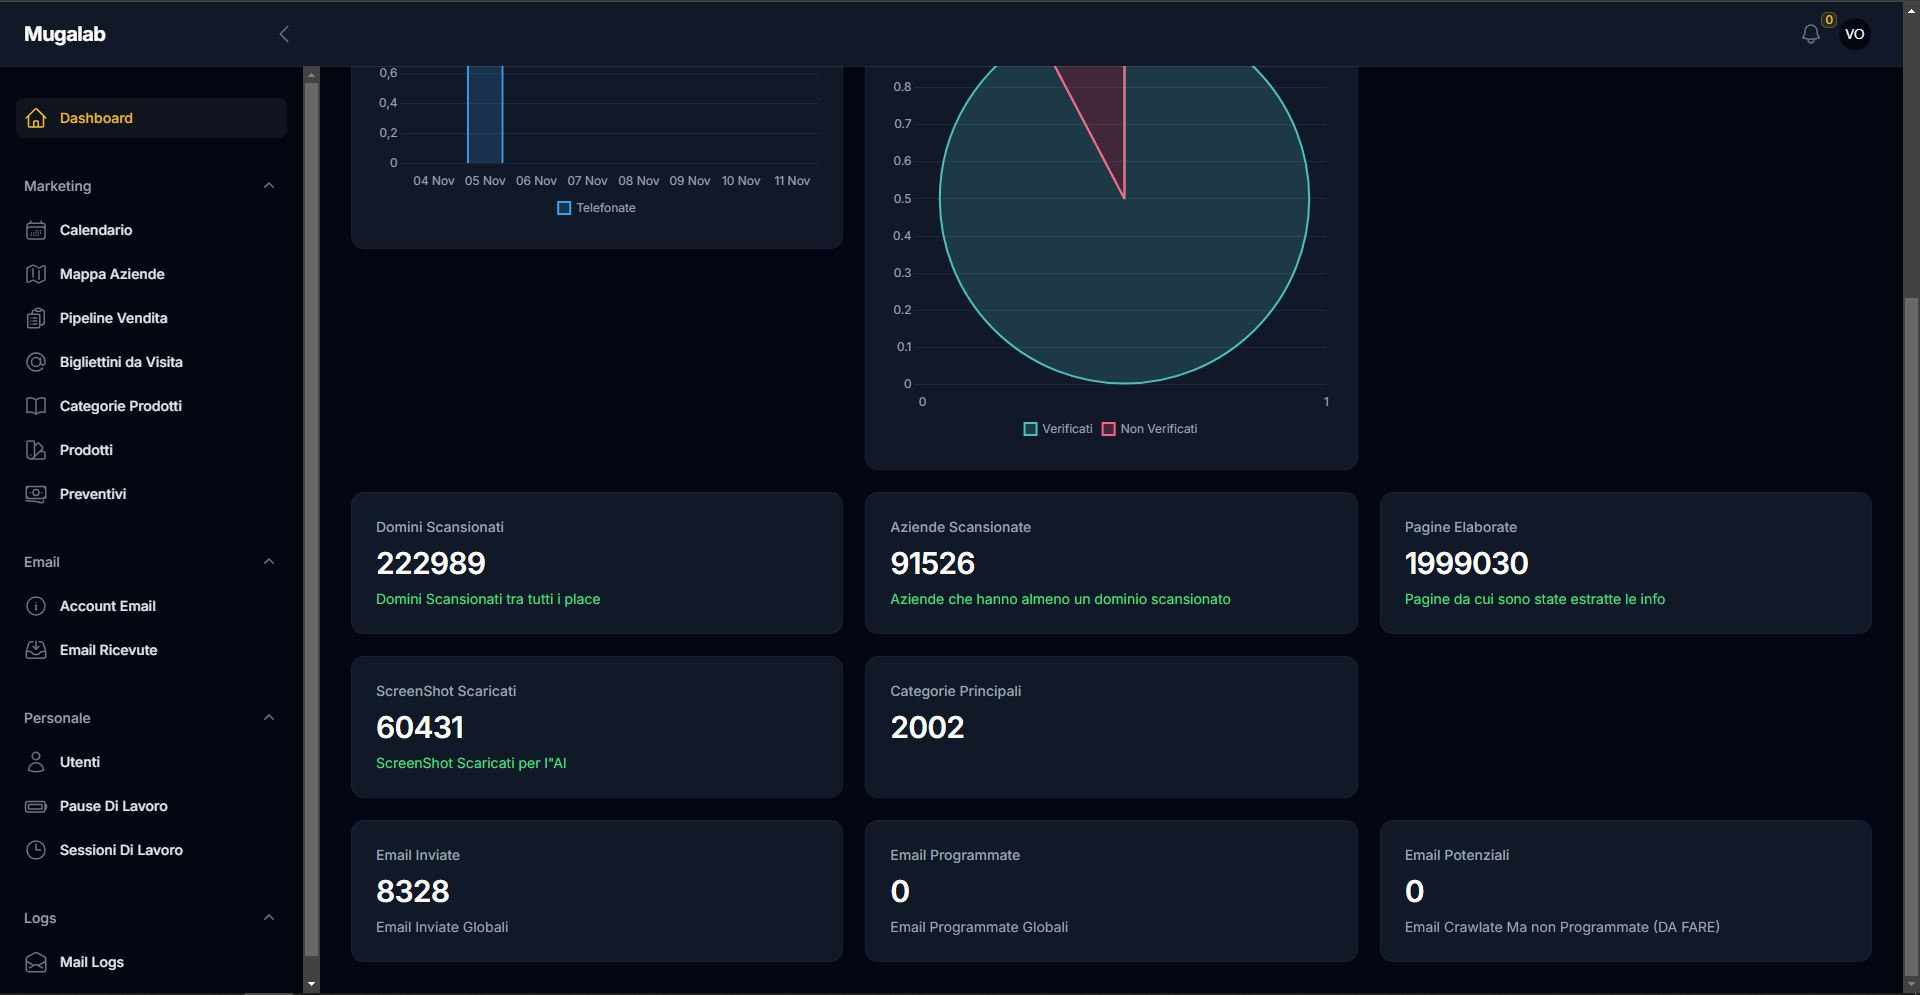
\includegraphics[width=0.8\columnwidth]{progetto/Home_page.png} 
        \caption{Homepage di SalesCRM}
        \label{fig:salesCRM-home}
      \end{figure}

    \item Il modulo contenente il calendario (Fig.~\ref{fig:salesCRM-calendario}) è utile per pianificare appuntamenti e visite.
    
    \begin{figure}[!h] 
        \centering 
        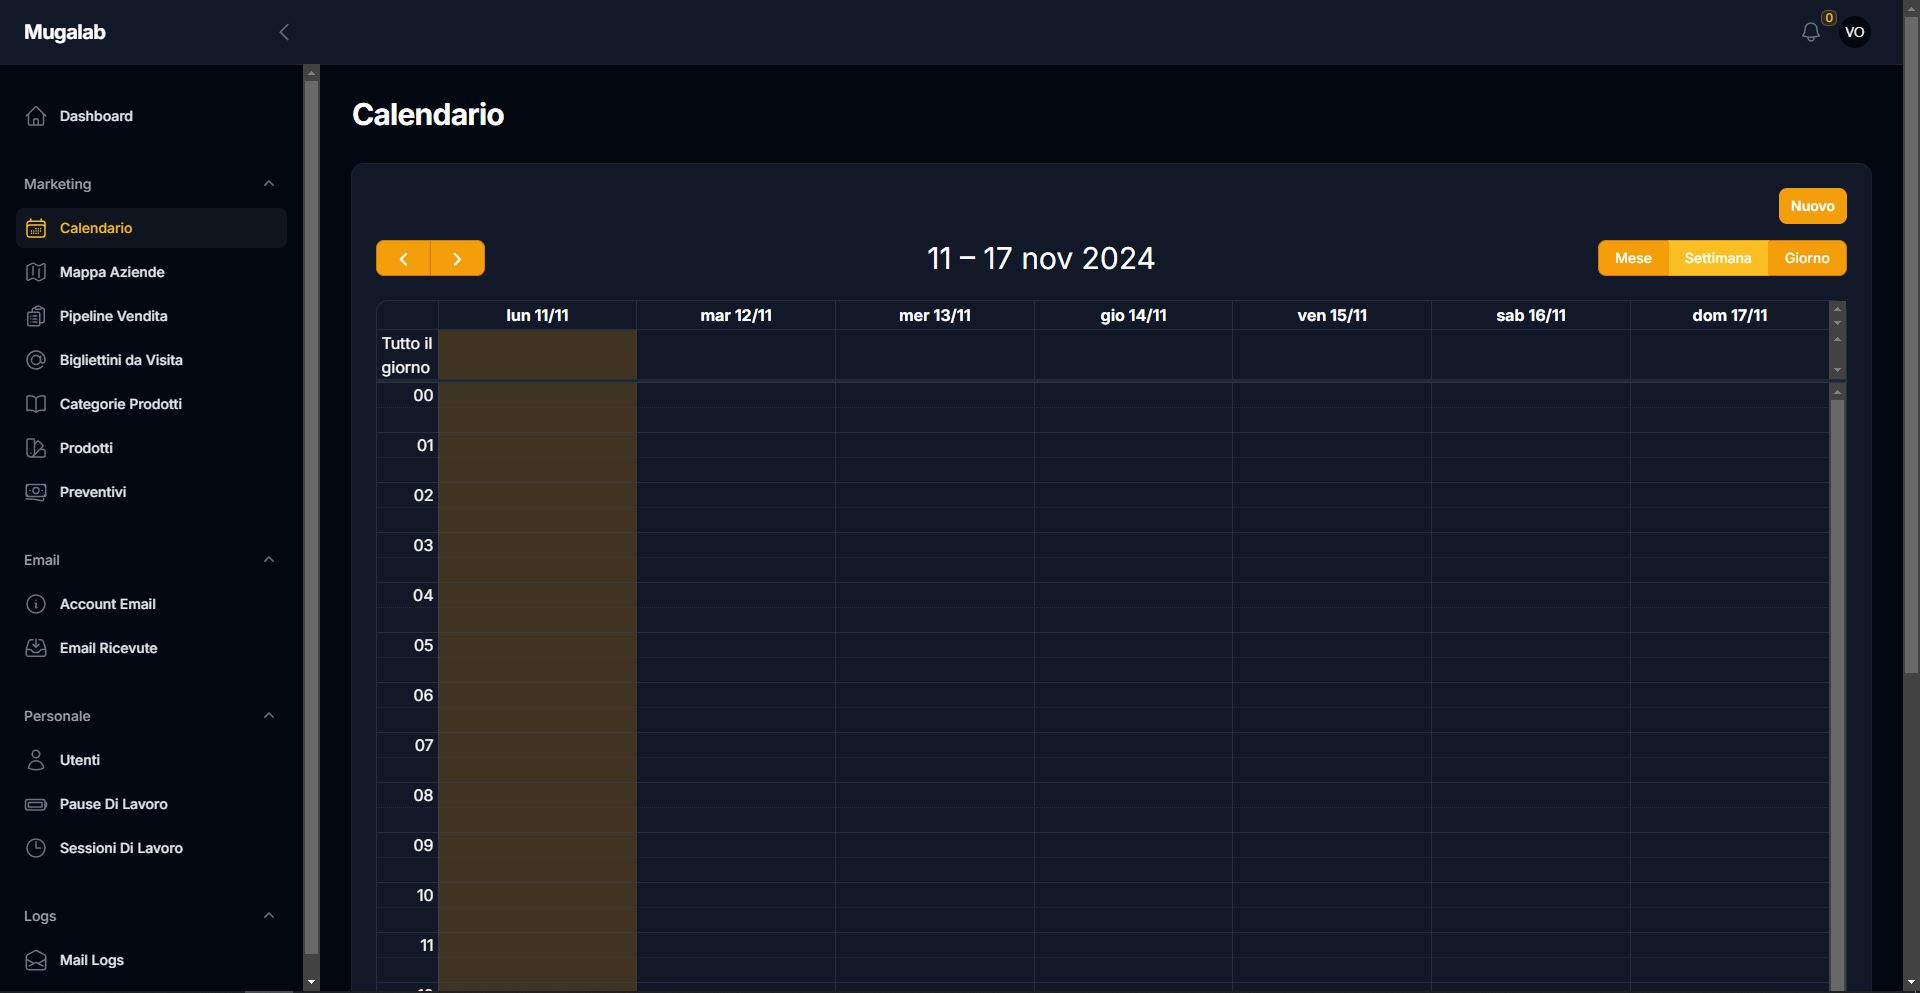
\includegraphics[width=0.8\columnwidth]{progetto/Calendario.png} 
        \caption{Calendario contenuto all'interno di SalesCRM}
        \label{fig:salesCRM-calendario}
      \end{figure}

    \item La sezione della mappa (Fig.~\ref{fig:salesCRM-mappa}) viene sfruttato per conoscere il posizionamento dei clienti e organizzare incontri locali.
    
    \begin{figure}[!h] 
        \centering 
        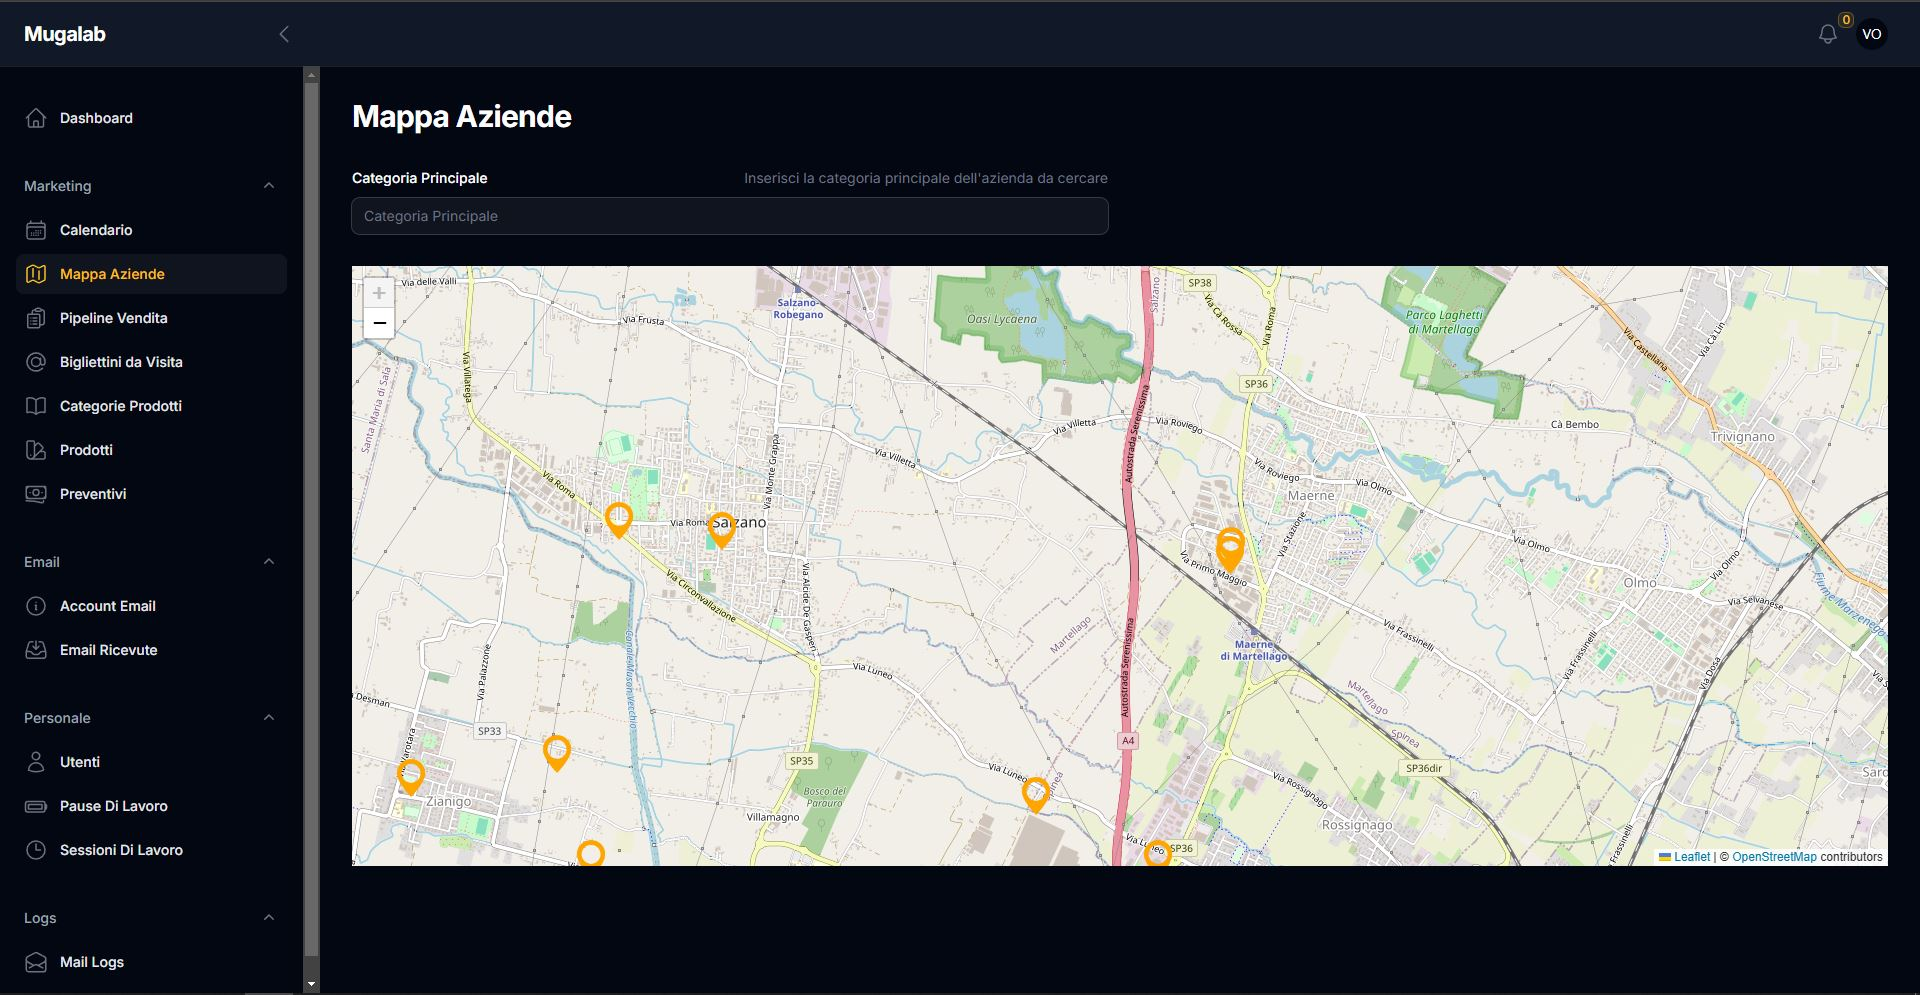
\includegraphics[width=0.8\columnwidth]{progetto/Mappa.png} 
        \caption{Mappa contenuta all'interno di SalesCRM}
        \label{fig:salesCRM-mappa}
      \end{figure}
    
\end{itemize}

\newpage

\subsection{Integrazione}
\begin{itemize}
    \item Raccolta di dati: l'applicativo ha una funzionalità di \emph{web scraping}\glsfirstoccur che raccoglie i link dei siti web di tutti i potenziali clienti, il compito del tirocinante è quello di creare un \emph{workflow} automatico che si integri con il \emph{web scraper} per acquisire screenshot delle varie pagine del sito web. 
    \item Clusterizzazione: la fase successiva alla raccolta dei dati consiste nello sviluppo di una IA addestrata in maniera non supervisionata che sia in grado di suddividere le varie immagini in \emph{cluster}, differenziati in base alle caratteristiche riconosciute in ogni sito. 
    \item IA classificativa: in seguito alla raccolta di un \emph{dataset}\glsfirstoccur di dimensioni congrue si procede alla suddivisione manuale degli screenshot precedentemente clusterizzati su una base qualitativa (siti migliorabili e siti ottimi); questo processo viene svolto con l'ottica dell'addestramento di una IA classificativa.
    L'IA addestrata in maniera supervisionata ha l'obiettivo di affidare un punteggio in valori centesimali a ogni sito. 
    \item Invio di e-mail automatizzato: l'automazione della posta elettronica procede con l'invio di e-mail personalizzate ai proprietari dei siti web che hanno ricevuto una valutazione scarsa, per offrire loro un servizio di miglioramento.
\end{itemize}

\section{Analisi e gestione dei rischi}
Durante l'analisi del progetto lo stagista ha individuato alcuni rischi in cui potrà incorrere.
Nella lista seguente sono elencati i rischi e le soluzioni ideate.\\

\begin{risk}{Rimodulazione dell'attività}
    \riskdescription{dopo un mese dall’inizio dello stage lo studente è stato riposizionato sul progetto attuale scartando il progetto precedente e trovandosi dunque con meno settimane a disposizione per la produzione}
    \risksolution{ridimensionamento delle attività e richieste di supporto più frequenti}
    \label{risk: tempistiche ristrette} 
\end{risk}

\begin{risk}{Approccio sperimentale}
    \riskdescription{il progetto prevede dei contributi originali e sperimentali per cui non sono disponibili soluzioni già pronte}
    \risksolution{auto apprendimento tramite tutorial online e richiesta di coinvolgimento di colleghi più esperti nell'ambito}
    \label{risk:conoscenze scarse} 
\end{risk}

\begin{risk}{Costo dell'Addestramento}
    \riskdescription{l'addestramento dell'intelligenza artificiale richiede l'utilizzo di potenti GPU di cui spesso l'hardware a disposizione è sprovvisto}
    \risksolution{utilizzo del server aziendale per l’addestramento su CPU, ottenendo un compromesso tra costi e tempo di addestramento}
    \label{risk:hardware} 
\end{risk}

\begin{risk}{Quantità di dati di training insufficiente}
    \riskdescription{l'IA necessita una grande quantità di dati in input per effettuare un training efficace}
    \risksolution{aumento manuale del \emph{dataset} e ricerca di \emph{dataset} già pronti online}
    \label{risk:hardware} 
\end{risk}

%AGGIUNGERE ALTRI RISCHI versioni dipendenti da altre

\newpage

\begin{risk}{Risultati della clusterizzazione non soddisfacenti}
    \riskdescription{il \emph{clustering} potrebbe risultare non conforme alle aspettative}
    \risksolution{valutare la quantità di cluster da creare e sperimentare con altri metodi di \emph{clustering}}
    \label{risk:hardware} 
\end{risk}


\begin{risk}{Overfitting del modello}
    \riskdescription{il modello IA fornisce valutazioni accurate solo per le immagini utilizzate durante il training}
    \risksolution{sperimentare con metodi per la risoluzione dell'\emph{overfit (dropout, cross-validation, ecc...)}}
    \label{risk:hardware} 
\end{risk}

\begin{risk}{Dipendenze delle librerie}
    \riskdescription{il progetto utilizza molte tecnologie e librerie differenti, è probabile che si presentino delle incompatibilità}
    \risksolution{utilizzo del minor numero possibile di librerie e verifica delle compatibilità prima dell'inizio della scrittura del codice}
    \label{risk:hardware} 
\end{risk}

\section{Obiettivi}
Gli obiettivi hanno lo scopo di delineare il percorso che lo studente deve affrontare per portare a termine il progetto nella maniera desiderata dall'azienda.
Sono suddivisibili in:
\begin{itemize}
    \item \textbf{O}: obbligatori
    \item \textbf{D}: desiderabili
    \item \textbf{F}: facoltativi
\end{itemize}

\begin{table}[h!]
    \centering
    \begin{tabularx}{0.8\textwidth}{|c|X|}
    \hline
    \textbf{Codice} & \textbf{Descrizione}\\
    \hline
    O01 & Implementare un sistema robusto per la cattura degli screenshot, assicurando l’integrazione con il database per l’archiviazione e l’analisi. \\
    \hline
    O02 & Garantire la creazione di una documentazione tecnica completa che supporti sia l’uso che la manutenzione  del sistema sviluppato. \\
    \hline
    O03 & Creazione di un IA in grado di suddividere in cluster i siti web. \\
    \hline
    O04 & Creazione di un IA classificativa in grado di assegnare un punteggio ai siti web analizzati.\\
    \hline
    D01 & Aggiungere la valutazione creata dall'IA nel database utilizzato dal CRM.\\
    \hline
    D02 & Automatizzare l'invio di e-mail alle aziende che hanno ottenuto una valutazione scarsa.\\
    \hline
    F01 & Migliorare la raccolta dei dati delle aziende dal web\\
    \hline
    F02 & Aggiornare automaticamente la valutazione dei siti web\\
    \hline
    \end{tabularx}
    \caption{Tabella degli obiettivi}
    \end{table}

%AGGIUNGERE SE HO TROPPE POCHE PAGINE
%\section{Pianificazione}


    \chapter{Analisi dei requisiti}
\label{cap:analisi-requisiti}

\intro{L'analisi dei requisiti è alla base della comprensione del prodotto da sviluppare, è utile per chiarire eventuali dubbi e per procedere in maniera spedita evitando perdite di tempo future}\\

\section{Casi d'uso}
Per rendere più chiari i casi d'uso sono stati utilizzati dei diagrammi di tipo \gls{UML}\glsfirstoccur.
Questo tipo di diagrammi descrivono funzioni e servizi forniti dal sistema agli attori che lo utilizzano.
Essendo il progetto l'implementazione di un \emph{\gls{workflow}} automatico, le interazioni dell'utente devono essere minime.
Per questo i casi d'uso sono pochi e molto sintetici.

\begin{figure}[!h] 
    \centering 
    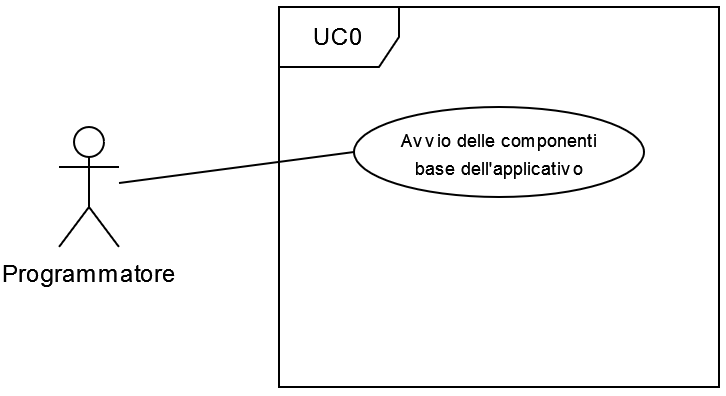
\includegraphics[width=0.9\columnwidth]{usecase/UC0.png} 
    \caption{Use Case - UC0: Scenario principale}
\end{figure}

\newpage

\begin{usecase}{0}{Scenario principale}
    \usecaseactors{Programmatore}
    \usecasepre{Il programmatore ha avviato l'ambiente di programmazione integrato}
    \usecasedesc{Avvio delle componenti base dell'applicativo}
    \usecasepost{Il sistema è pronto per eseguire il \emph{\gls{workflow}}}
    \label{uc:scenario-principale}
\end{usecase}

\begin{figure}[!h] 
    \centering 
    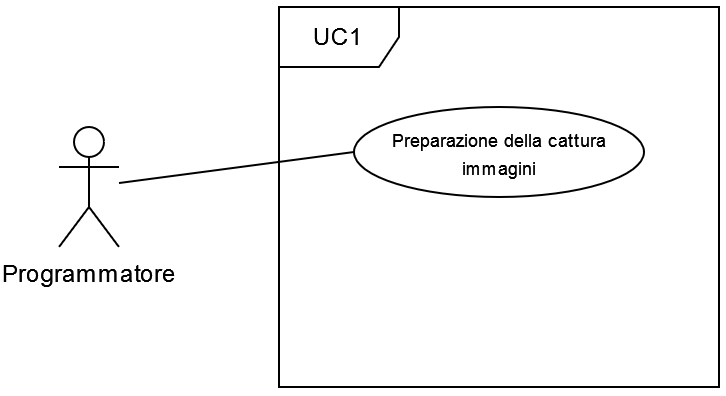
\includegraphics[width=0.9\columnwidth]{usecase/UC1.png} 
    \caption{Use Case - UC1: Acquisizione screenshot}
\end{figure}

\begin{usecase}{1}{Acquisizione screenshot} 
    \usecaseactors{Programmatore} 
    \usecasepre{Il \emph{web scraper} ha già raccolto i link alle pagine dei siti web delle aziende} 
    \usecasedesc{Il programmatore prepara il \emph{\gls{workflow}} per acquisire in maniera automatica gli screenshot delle pagine raccolte in precedenza} 
    \usecasepost{Gli screenshot vengono salvati nel database, pronti per la fase di analisi e classificazione} 
    \label{uc:acquisizione-screenshot} 
\end{usecase}
 
\newpage

\begin{figure}[!h] 
    \centering 
    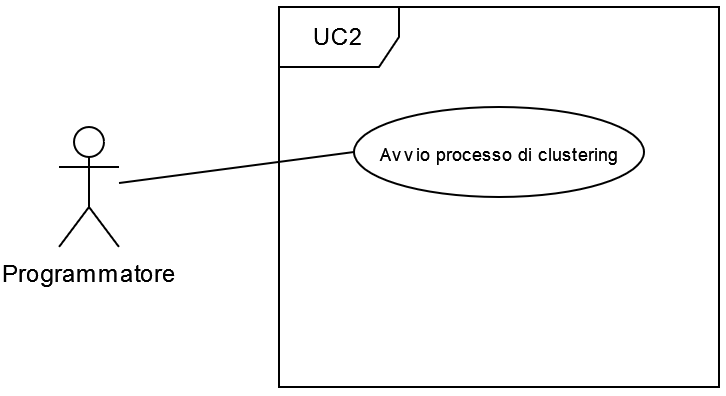
\includegraphics[width=0.9\columnwidth]{usecase/UC2.png} 
    \caption{Use Case - UC2: Clusterizzazione degli screenshot}
\end{figure}

\begin{usecase}{2}{Clusterizzazione degli screenshot} 
    \usecaseactors{Programmatore} 
    \usecasepre{Gli screenshot delle pagine sono stati acquisiti e salvati nel database}
    \usecasedesc{Il programmatore avvia il processo di \emph{clustering}, che organizza gli screenshot in \emph{cluster} in base alle \emph{\gls{feature}\glsfirstoccur estratte}}
    \usecasepost{Gli screenshot vengono clusterizzati e inseriti in apposite cartelle} 
    \label{uc:clusterizzazione-screenshot} 
\end{usecase}

\begin{figure}[!h] 
    \centering 
    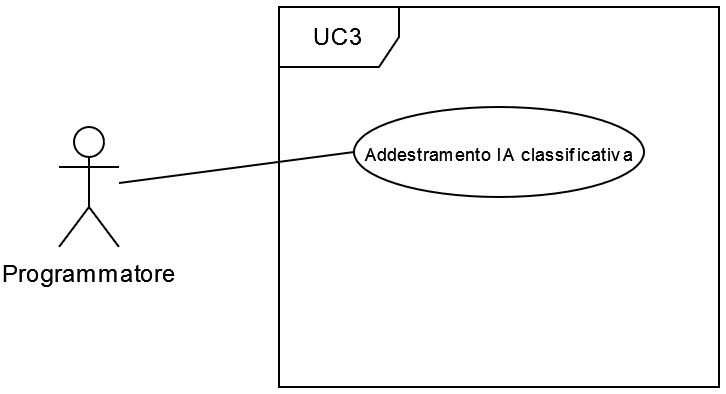
\includegraphics[width=0.9\columnwidth]{usecase/UC3.png} 
    \caption{Use Case - UC3: IA classificativa}
\end{figure}

\newpage

\begin{usecase}{3}{Valutazione qualitativa e classificazione} 
    \usecaseactors{Programmatore} 
    \usecasepre{Gli screenshot sono stati inseriti in cartelle} 
    \usecasedesc{Lo sviluppatore addestra l'IA classificativa sfruttando i cluster precedentemente creati, e creando un \emph{\gls{dataset}}} 
    \usecasepost{Ogni sito ottiene un punteggio qualitativo che viene salvato nel database per operazioni future} 
    \label{uc:IA-classificativa} 
\end{usecase}

\begin{figure}[!h] 
    \centering 
    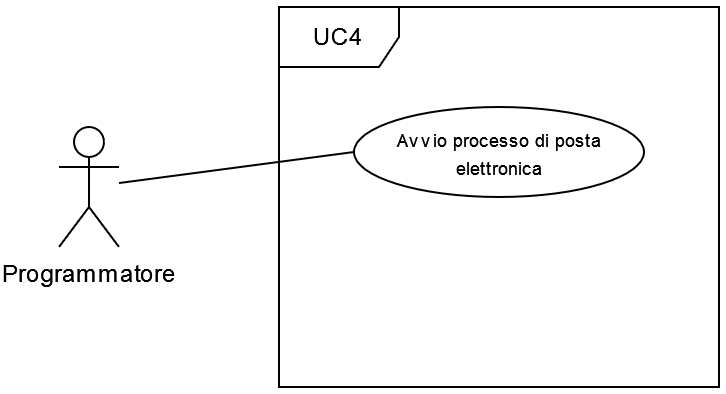
\includegraphics[width=0.9\columnwidth]{usecase/UC4.png} 
    \caption{Use Case - UC4: invio e-mail}
\end{figure}


\begin{usecase}{4}{Automazione dell'invio di e-mail} 
    \usecaseactors{Programmatore} 
    \usecasepre{I siti web contenuti nel database hanno ricevuto una valutazione} 
    \usecasedesc{Il sistema invia automaticamente e-mail personalizzate ai proprietari dei siti con punteggi di qualità bassi, offrendo servizi di miglioramento} 
    \usecasepost{Le e-mail vengono inviate con successo ai destinatari} 
    \label{uc:invio-e-mail} 
\end{usecase}


    \chapter{Strumenti e tecnologie}
\label{cap:strumenti-tecnologie}

\intro{L'obiettivo principale di questo capitolo è l'illustrazione delle tecnologie e degli strumenti ausiliari utilizzati per raggiungere lo scopo finale del progetto}\\

\section{Strumenti}
\label{sec:strumenti}
Gli strumenti di supporto adoperati per il progetto sono elencati nella lista seguente.

\subsection{Visual Studio Code}
\textbf{Visual Studio Code} (Fig.~\ref{fig:logo-vscode}): è un ambiente di sviluppo integrato, disponibile per Linux, macOS e Windows. 
È un'applicazione che supporta la maggior parte dei linguaggi di programmazione ed è quindi molto vantaggiosa per lavorare a un progetto multi linguaggio senza dover cambiare ambiente.
Un'altra delle funzionalità principali è la fornitura di numerose estensioni che semplificano il processo di scrittura e verifica del codice.

\begin{figure}[!h] 
    \centering 
    
\includegraphics[width=0.4\columnwidth]{tecnologie/visual-studio-logo.png} 
    \caption{Logo di Visual Studio Code}
    \label{fig:logo-vscode}
  \end{figure}

\newpage

\subsection{PhpMyAdmin}
\textbf{PhpMyAdmin} (Fig.~\ref{fig:logo-phpmyadmin}): è una \emph{\gls{web app}}\glsfirstoccur scritta utilizzando il linguaggio di programmazione PHP, che offre la capacità di gestione di un database MySQL attraverso un \emph{browser} qualsiasi. Consente la creazione di tabelle, l'inserimento, la modifica e l'interrogazione dei dati.
Fornisce un'interfaccia grafica per la visione d'insieme e per le operazioni amministrative.

\begin{figure}[!h] 
      \centering 
      
\includegraphics[width=0.4\columnwidth]{tecnologie/phpmyadmin-logo.png} 
      \caption{Logo di phpMyAdmin}
    \label{fig:logo-phpmyadmin}
  \end{figure}

\subsection{remoteripple}
\textbf{Remote Ripple} (Fig.~\ref{fig:logo-remoteripple}): è un software per l'accesso remoto, che viene utilizzato dallo studente per avviare i programmi presenti nel server aziendale.
    
\begin{figure}[!h] 
    \centering 
    
\includegraphics[width=0.3\columnwidth]{tecnologie/remote-ripple-logo.png} 
    \caption{Logo di Remote Ripple}
    \label{fig:logo-remoteripple}
  \end{figure}


\newpage

\section{Tecnologie}
\label{sec:tecnologie-strumenti}

Nelle sezioni seguenti viene data una spiegazione di tutte le tecnologie utilizzate.

\subsection{Python}

\subsubsection{Versione: 3.9.0}
Python (Fig.~\ref{fig:logo-python}) è un linguaggio di programmazione ampiamente utilizzato in settori come il \emph{data mining} e l'intelligenza artificiale. 
Offre solide basi per l'integrazione con disparati linguaggi, ma il vantaggio più di risalto è la presenza di numerose librerie che aiutano lo sviluppatore a velocizzare il processo di codifica; in particolare sono state utilizzate le seguenti librerie:

\subsubsection{\label{tec:tensorflow}Tensorflow-gpu 2.10.1}

TensorFlow è un \emph{\gls{framework}}\glsfirstoccur utilizzato per il \emph{machine learning}, su di esso si basa tutta la struttura del progetto.\\
L'unità di base del \emph{\gls{framework}} è il tensore, ossia un vettore di n dimensioni, tutte le operazioni possibili vengono eseguite su elementi appartenenti a questo tipo.
Inoltre contiene modelli preaddestrati molto utili per eseguire determinate operazioni in maniera più rapida. 
Viene utilizzata la versione 2.10 perché è l'ultima ad avere il supporto per GPU su sistema operativo Windows.

\subsubsection{Keras 2.10.0}
Keras è un \emph{\gls{API}\glsfirstoccur (Application Programming Interface)} sviluppata per rendere la codifica di IA più semplice per la comprensione umana. 
Minimizza le azioni richieste all'utente per i casi d'uso più comuni, rendendo l'utilizzo di \emph{\gls{framework}} come JAX, TensorFlow e PyTorch più \emph{user friendly}.

\subsubsection{Scikit-Learn 1.5.2}
Scikit-learn è una libreria che offre semplici \emph{tool} utili per la classificazione, la regressione, il clustering, eccetera.

\subsubsection{Matplotlib 3.9.2}
Matplotlib è una libreria che viene utilizzata per la stampa dei grafici ottenuti durante le varie compilazioni. 

\subsubsection{Numpy 1.26.4}
Numpy è il pacchetto che si occupa della gestione di \emph{array} multi dimensionali fornendo anche un'ampia gamma di funzioni matematiche da applicare agli stessi.

\subsubsection{OpenCV-python 4.10.0}
OpenCV è una libreria utilizzata per sviluppare applicazioni di tipo \emph{\gls{computer vision}}\glsfirstoccur. Nell'ambito del progetto il suo scopo primario è l'elaborazione delle immagini per adattarle all'utilizzo da parte delle IA. 

\subsubsection{Pyppeteer 2.0.0}
Pyppeteer è una libreria di automazione per browser basati su chromium.

\begin{figure}[!h] 
  \centering 
  
\includegraphics[width=0.8\columnwidth]{tecnologie/python-librerie.png} 
  \caption{Python e librerie utilizzate}
  \label{fig:logo-python}
\end{figure}

\newpage

\subsection{\label{tec:cuda}CUDA}
\subsubsection{Versione: 11.2}
CUDA (Fig.~\ref{fig:logo-cuda}) è un \emph{toolkit} che fornisce un ambiente di sviluppo in grado di creare applicazioni che sfruttino a pieno le GPU di NVIDIA.
Nel caso di studio CUDA è un elemento portante in quanto fornisce a Python e alle sue librerie la capacità di eseguire calcoli in maniera più rapida utilizzando la GPU.
Le GPU hanno un'architettura diversa rispetto alle CPU che consente loro di eseguire parallelamente più operazioni, per questo sono molto portate per l'addestramento delle IA.
La versione 11.2 viene utilizzata perché è l'unica compatibile con \nameref{tec:tensorflow}.

\begin{figure}[!h] 
  \centering 
  
\includegraphics[width=0.5\columnwidth]{tecnologie/cuda-logo.png} 
  \caption{Logo di CUDA}
  \label{fig:logo-cuda}
\end{figure}


\subsection{\label{tec:docker}Docker}
\subsubsection{Versione: 27.2.0}
Docker (Fig.~\ref{fig:logo-docker}) è un sistema che consente di semplificare lo sviluppo delle applicazioni fornendo un ambiente isolato e facilmente riproducibile. Tale ambiente viene definito come container, al suo interno vengono eseguite le immagini di tutti i componenti necessari per il funzionamento dell'applicativo; senza che sia necessario installarli sulla propria macchina.

\begin{figure}[!h] 
  \centering 
  
\includegraphics[width=0.5\columnwidth]{tecnologie/docker-logo.png} 
  \caption{Logo di Docker}
  \label{fig:logo-docker}
\end{figure}


\subsection{\label{tec:ddev}DDEV}
\subsubsection{Versione: 1.23.2}
DDEV (Fig.~\ref{fig:logo-ddev}) è un \emph{tool} per velocizzare il lancio di ambienti di sviluppo web in locale; consente di utilizzare il \emph{\gls{workflow}} di \nameref{tec:docker} in maniera più rapida.

\begin{figure}[!h] 
  \centering 
  
\includegraphics[width=0.25\columnwidth]{tecnologie/ddev-logo.png} 
  \caption{Logo di DDEV}
  \label{fig:logo-ddev}
\end{figure}



\subsection{\label{tec:wsl}WSL}
\subsubsection{Versione: 2.3.24.0}
WSL (Fig.~\ref{fig:logo-wsl}) è un sottosistema che viene utilizzato per eseguire applicazioni create per il sistema operativo Linux su Windows.

\begin{figure}[!h] 
  \centering 
  
\includegraphics[width=0.3\columnwidth]{tecnologie/wsl-logo.png} 
  \caption{Logo di WSL}
  \label{fig:logo-wsl}
\end{figure}

\subsection{\label{tec:Laravel}Laravel}
\subsubsection{Versione: 11.29.0}
Laravel (Fig.~\ref{fig:logo-laravel}) è un \emph{\gls{framework}} ideato per la creazione di \emph{\gls{web app}} scritto in PHP.
Tra i suoi vantaggi abbiamo la semplicità della sintassi, il supporto continuo della community e la presenza di numerosi tutorial che è fondamentale per fornire a sviluppatori alle prime armi l'aiuto necessario.
Laravel si basa sul pattern architetturale \emph{MVC (Model View Controller)}:
\begin{itemize}
  \item \textbf{Model}: accede ai dati contenuti nell'applicativo.
  \item \textbf{View}: mostra i dati contenuti nel model e gestisce le interazioni con gli utenti.  
  \item \textbf{Controller}: riceve le operazioni degli utenti e modifica di conseguenza i dati contenuti nel model e la visualizzazione mostrata dalla view.
\end{itemize}

\begin{figure}[!h] 
  \centering 
  
\includegraphics[width=0.3\columnwidth]{tecnologie/logo-laravel.png} 
  \caption{Logo di Laravel}
  \label{fig:logo-laravel}
\end{figure}

\newpage 

\subsection{\label{tec:Filament}Filament}
\subsubsection{Versione: 3.2.121}
Filament (Fig.~\ref{fig:logo-filament}) è un \emph{\gls{framework}} basato su \nameref{tec:Laravel} che fornisce la possibilità di generare componenti per l'interfaccia grafica (Fig.~\ref{fig:gui-filament}) in maniera rapida.

\begin{figure}[!h] 
  \centering 
  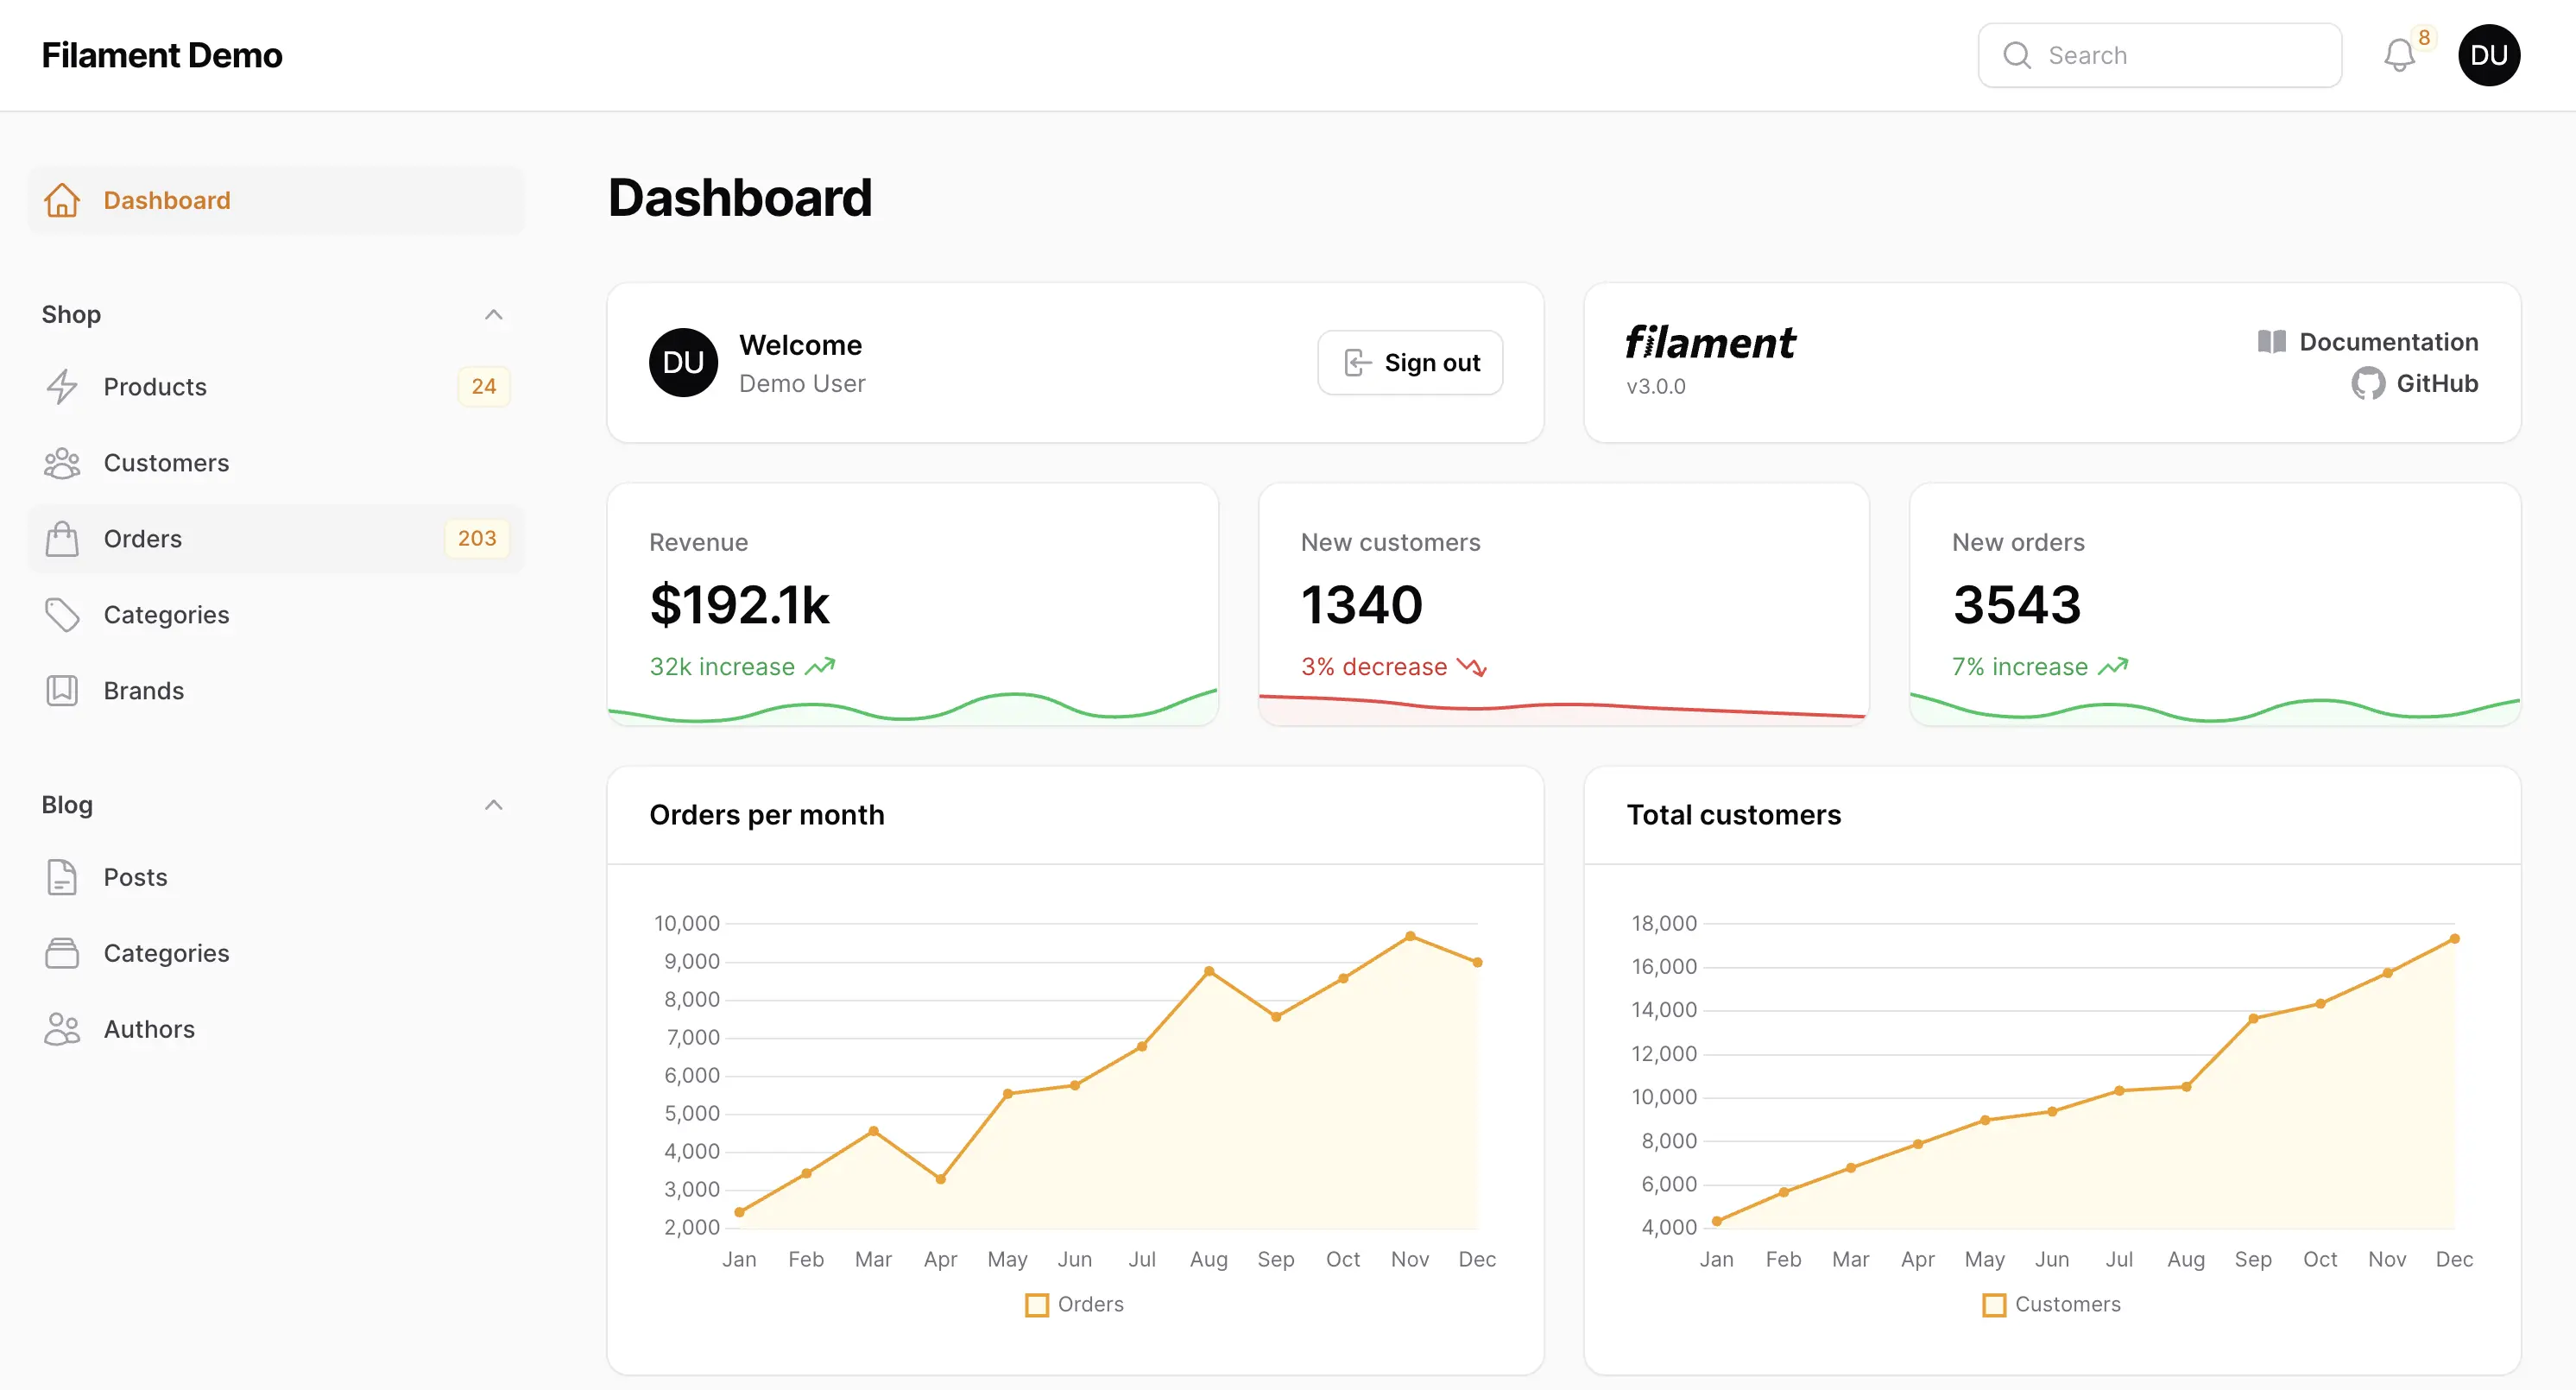
\includegraphics[width=0.8\columnwidth]{tecnologie/filament-demo.png} 
  \caption{Esempio di interfaccia grafica creata in Filament}
  \label{fig:gui-filament}
\end{figure}

\begin{figure}[!h] 
  \centering 
  
\includegraphics[width=0.3\columnwidth]{tecnologie/filament-logo.png} 
  \caption{Logo di Filament}
  \label{fig:logo-filament}
\end{figure}

\newpage

\subsection{\label{tec:mysql}MySQL}
\subsubsection{Versione: 8.0.36}
MySQL (Fig.~\ref{fig:logo-mysql}) è un database relazionale \emph{\gls{open source}}.

\begin{figure}[!h] 
  \centering 
  
\includegraphics[width=0.3\columnwidth]{tecnologie/mysql-logo.png} 
  \caption{Logo di MySQL}
  \label{fig:logo-mysql}
\end{figure}

%AGGIUNGERE DA QUALCHE PARTE LE DIPENDENZE TRA LIBRERIE E VERSIONI


    \chapter{Machine learning}
\label{cap:teoria}
\intro{Per comprendere al meglio gli argomenti trattati nel capitolo successivo è necessaria un'introduzione teorica}\\Il \emph{machine learning} è un'applicazione della statistica che si concentra sullo sviluppo di algoritmi in grado di imparare dai dati che vengono loro forniti in \emph{input}.
Da un punto di vista più filosofico il \emph{machine learning} è interessante perché sviluppando la nostra conoscenza su di esso stiamo di conseguenza migliorando la nostra comprensione dei principi su cui si sorregge l'intelligenza \footcite[p.~97]{Goodfellow-et-al-2016}.\\Gli algoritmi di \emph{machine learning} si suddividono in due categorie principali:

\begin{itemize}
    \item \textbf{Apprendimento supervisionato}: gli algoritmi che appartengono a questa categoria apprendono quali risultati generare seguendo la guida di un set di dati etichettati e con un \emph{output} predefinito\footcite{site:machine-learning}.

    \item \textbf{Apprendimento non supervisionato}: gli algoritmi non supervisionati, anche conosciuti come apprendimento automatico, analizzano e raggruppano \emph{\gls{dataset}} non etichettati. Questi algoritmi riconoscono raggruppamenti di dati (\emph{cluster}) senza la necessità dell'intervento umano\footcite{site:machine-learning}.
\end{itemize}
Tali algoritmi vengono utilizzati nel progetto per il processo di classificazione.\\
La classificazione è un metodo che consente di prevedere a quale classe un determinato \emph{input} appartenga. 
Quindi generalizzando un'entità viene rappresentata come vettore in uno spazio delle \emph{\gls{feature}}, tipicamente \( R^n \), successivamente vengono eseguite delle operazioni sul vettore che producono un valore preso da un insieme di etichette L noto a priori, il classificatore è quindi una funzione \( R^n \rightarrow L \).\\Un classico esempio di classificazione è fornito dal \emph{\gls{dataset}} Iris\footcite{site:iris-dataset}, è uno dei primi \emph{\gls{dataset}} utilizzati in letteratura per sperimentare i metodi di classificazione; contiene 3 classi composte da 50 istanze ciascuna, ogni classe si riferisce a un tipologia differente di iris (Fig.~\ref{fig:iris-images}).

\begin{figure}[!h] 
    \centering 
    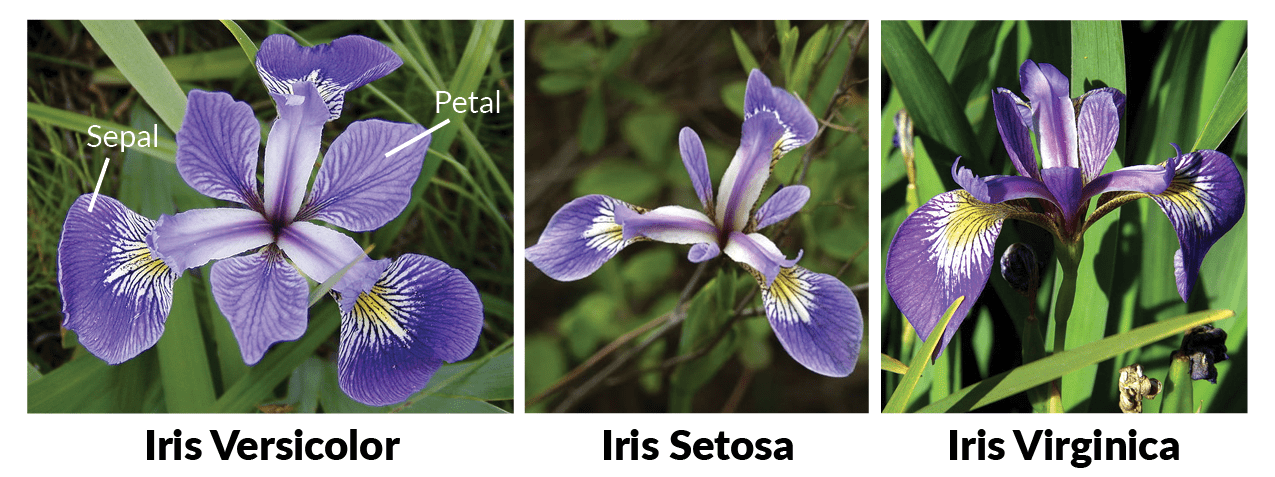
\includegraphics[width=0.8\columnwidth]{teoria/iris-images.png} 
    \caption{Tre tipologie di pianta}
    \label{fig:iris-images}
  \end{figure}
In fase di addestramento vengono utilizzate le \emph{\gls{feature}} e le etichette (Fig.~\ref{fig:iris-schema}) di ciascuna pianta e in fase di test l'algoritmo utilizza le caratteristiche apprese per eseguire una classificazione su dati che non ha ricevuto durante il \emph{traininig}.

\begin{figure}[!h] 
    \centering 
    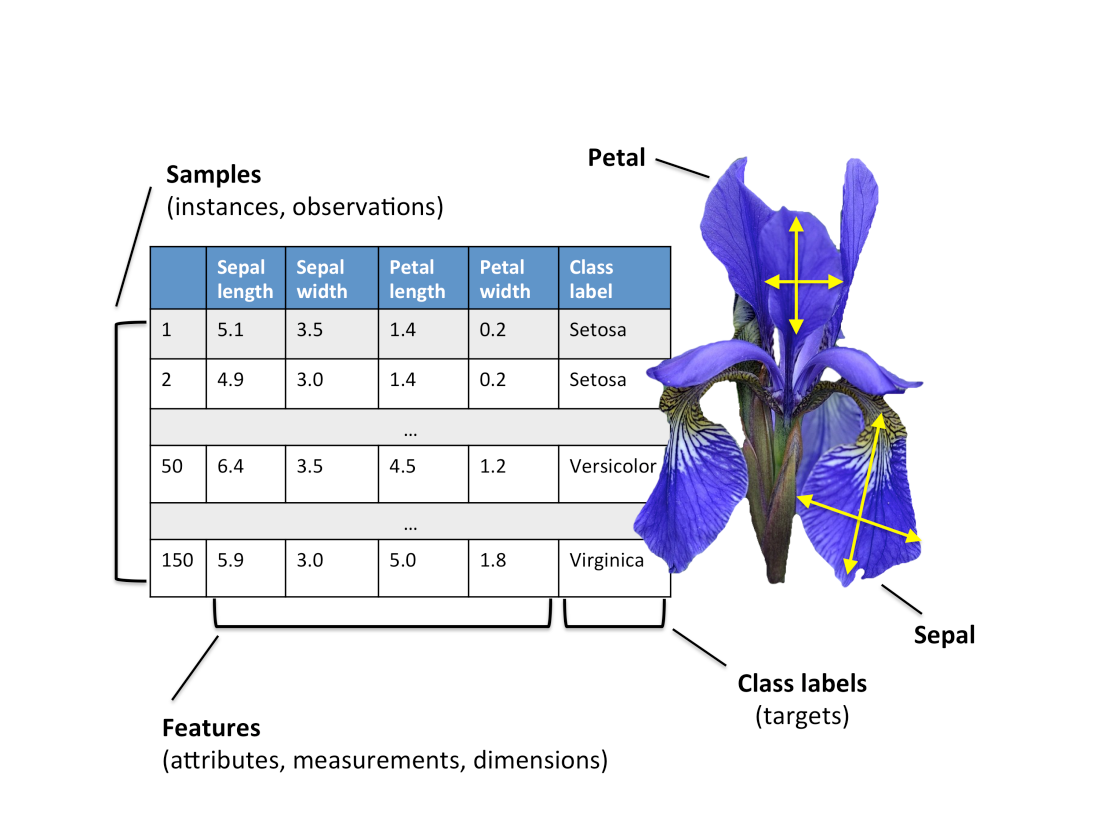
\includegraphics[width=0.8\columnwidth]{teoria/iris-schema.png} 
    \caption{Schema delle feature}
    \label{fig:iris-schema}
  \end{figure}
L'introduzione al \emph{machine learning} è utile per presentare le applicazioni di tale disciplina utilizzate ai fini del progetto:
\begin{itemize}
    \item \textbf{Clustering}
    \item \textbf{PCA}
    \item \textbf{Reti neurali}
    \item \textbf{Deep learning}
    \item \textbf{Autoencoder}
\end{itemize}
Gli elementi citati in precedenza vengono introdotti e trattati nelle sezioni seguenti.

\newpage

\section{K-means}
Il K-means è un algoritmo non supervisionato che viene utilizzato per il \emph{clustering}, ossia per la suddivisione del \emph{\gls{dataset}} in gruppi che contengono caratteristiche simili.
Suddivide un set di dati in gruppi simili sulla base della distanza tra i loro centroidi. 
Il centroide, è la media di tutti i punti presenti all'interno del \emph{cluster}.\\Il numero K sta a indicare quanti \emph{cluster} dovranno essere assegnati dall'algoritmo, più il numero di \emph{cluster} è elevato più essi saranno piccoli e dettagliati al contrario se i \emph{cluster} sono pochi il risultato saranno dei \emph{cluster} più grandi ma meno dettagliati (Fig.~\ref{fig:k-means}).

\begin{figure}[!h] 
    \centering 
    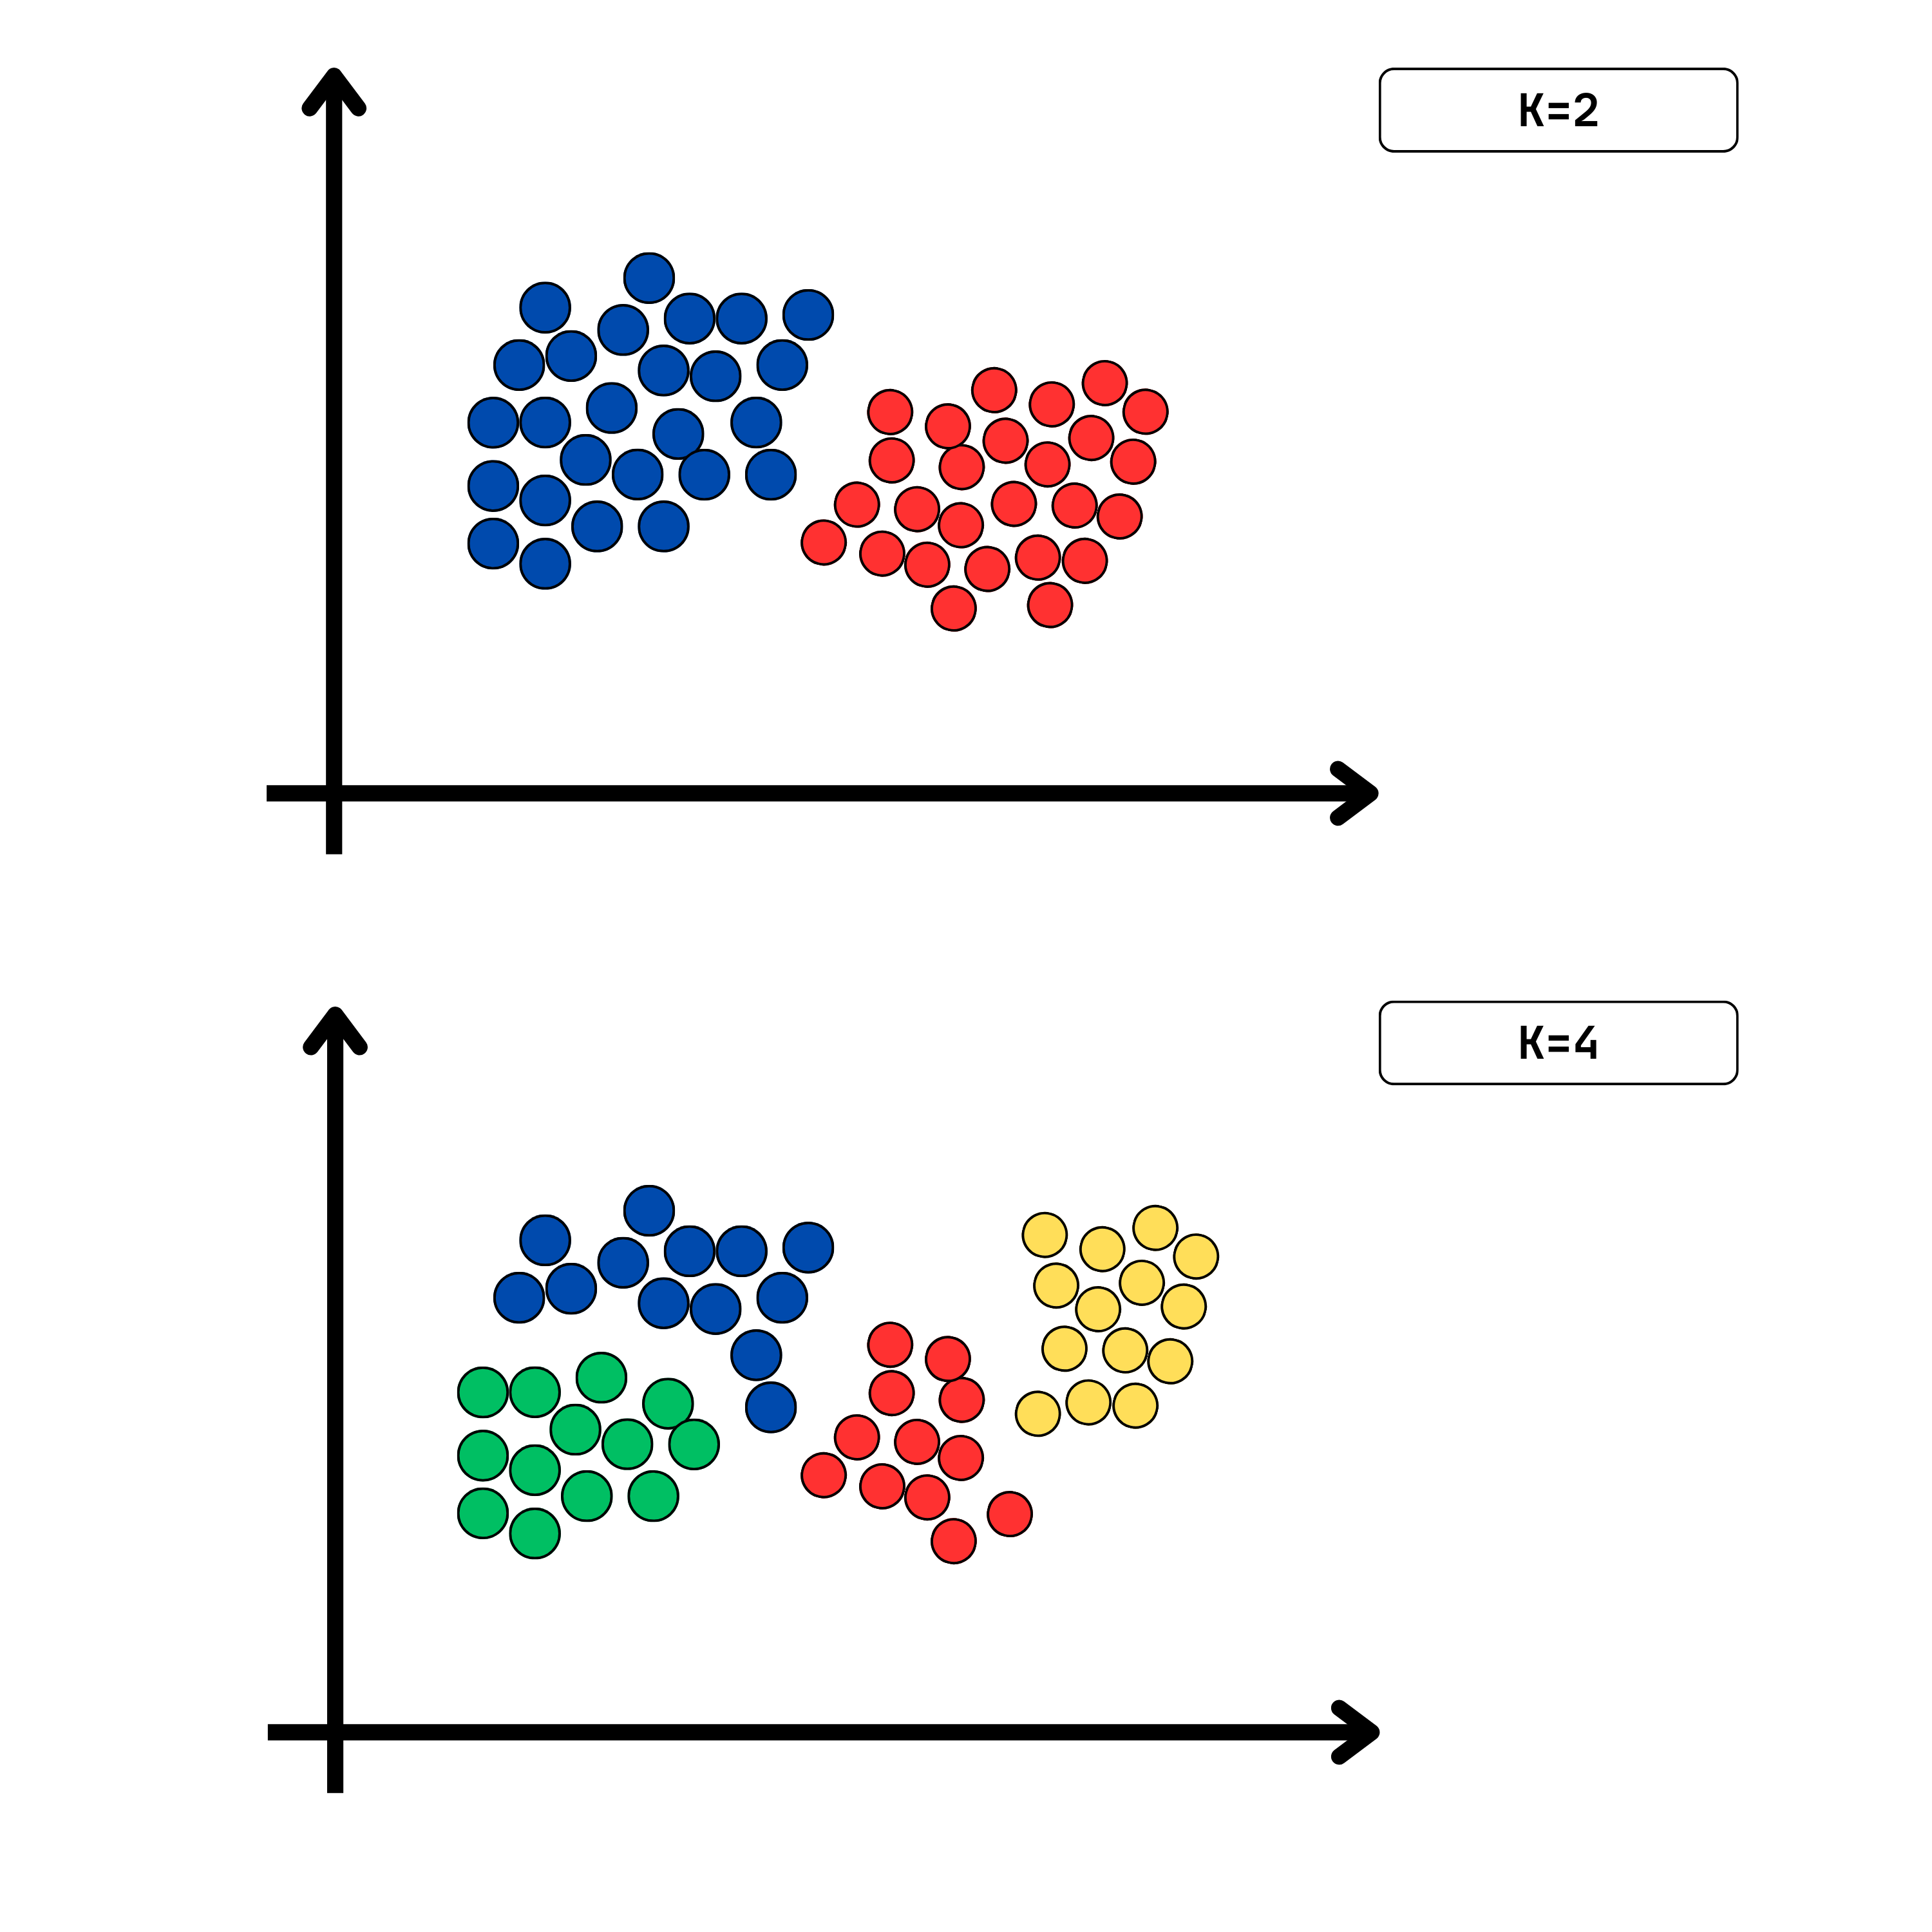
\includegraphics[width=0.7\columnwidth]{teoria/k-means.png} 
    \caption{Esempio di clustering}
    \label{fig:k-means}
  \end{figure}
Ad esempio se volessimo clusterizzare un insieme di animali composto da mammiferi e volatili utilizzando K=2 l'algoritmo creerebbe due \emph{cluster} uno contenente i mammiferi e uno i volatili  (\emph{cluster} grandi e poco dettagliati).
Se aumentassimo il numero di \emph{cluster} l'algoritmo sarebbe in grado di essere più specifico andando a creare una quantità molto più elevata di \emph{cluster} ben dettagliati contenenti meno elementi.
Quindi è importante scegliere con cura il numero iniziale K da assegnare, per semplificare questa operazione esistono dei metodi di supporto:
\begin{itemize}
    \item Il metodo del gomito sfrutta l’inerzia, ossia la somma delle distanze al quadrato dei punti dal centroide \emph{(SSE, Sum of Squared Errors)}. Con l'aumento dei \emph{cluster}, l’inerzia diminuisce, ma dopo un certo punto, la riduzione diventa superflua, venendo a creare una curva a gomito. Il punto in cui la curva si piega indica il numero di \emph{cluster} da utilizzare.
    
    \begin{figure}[!h] 
        \centering 
        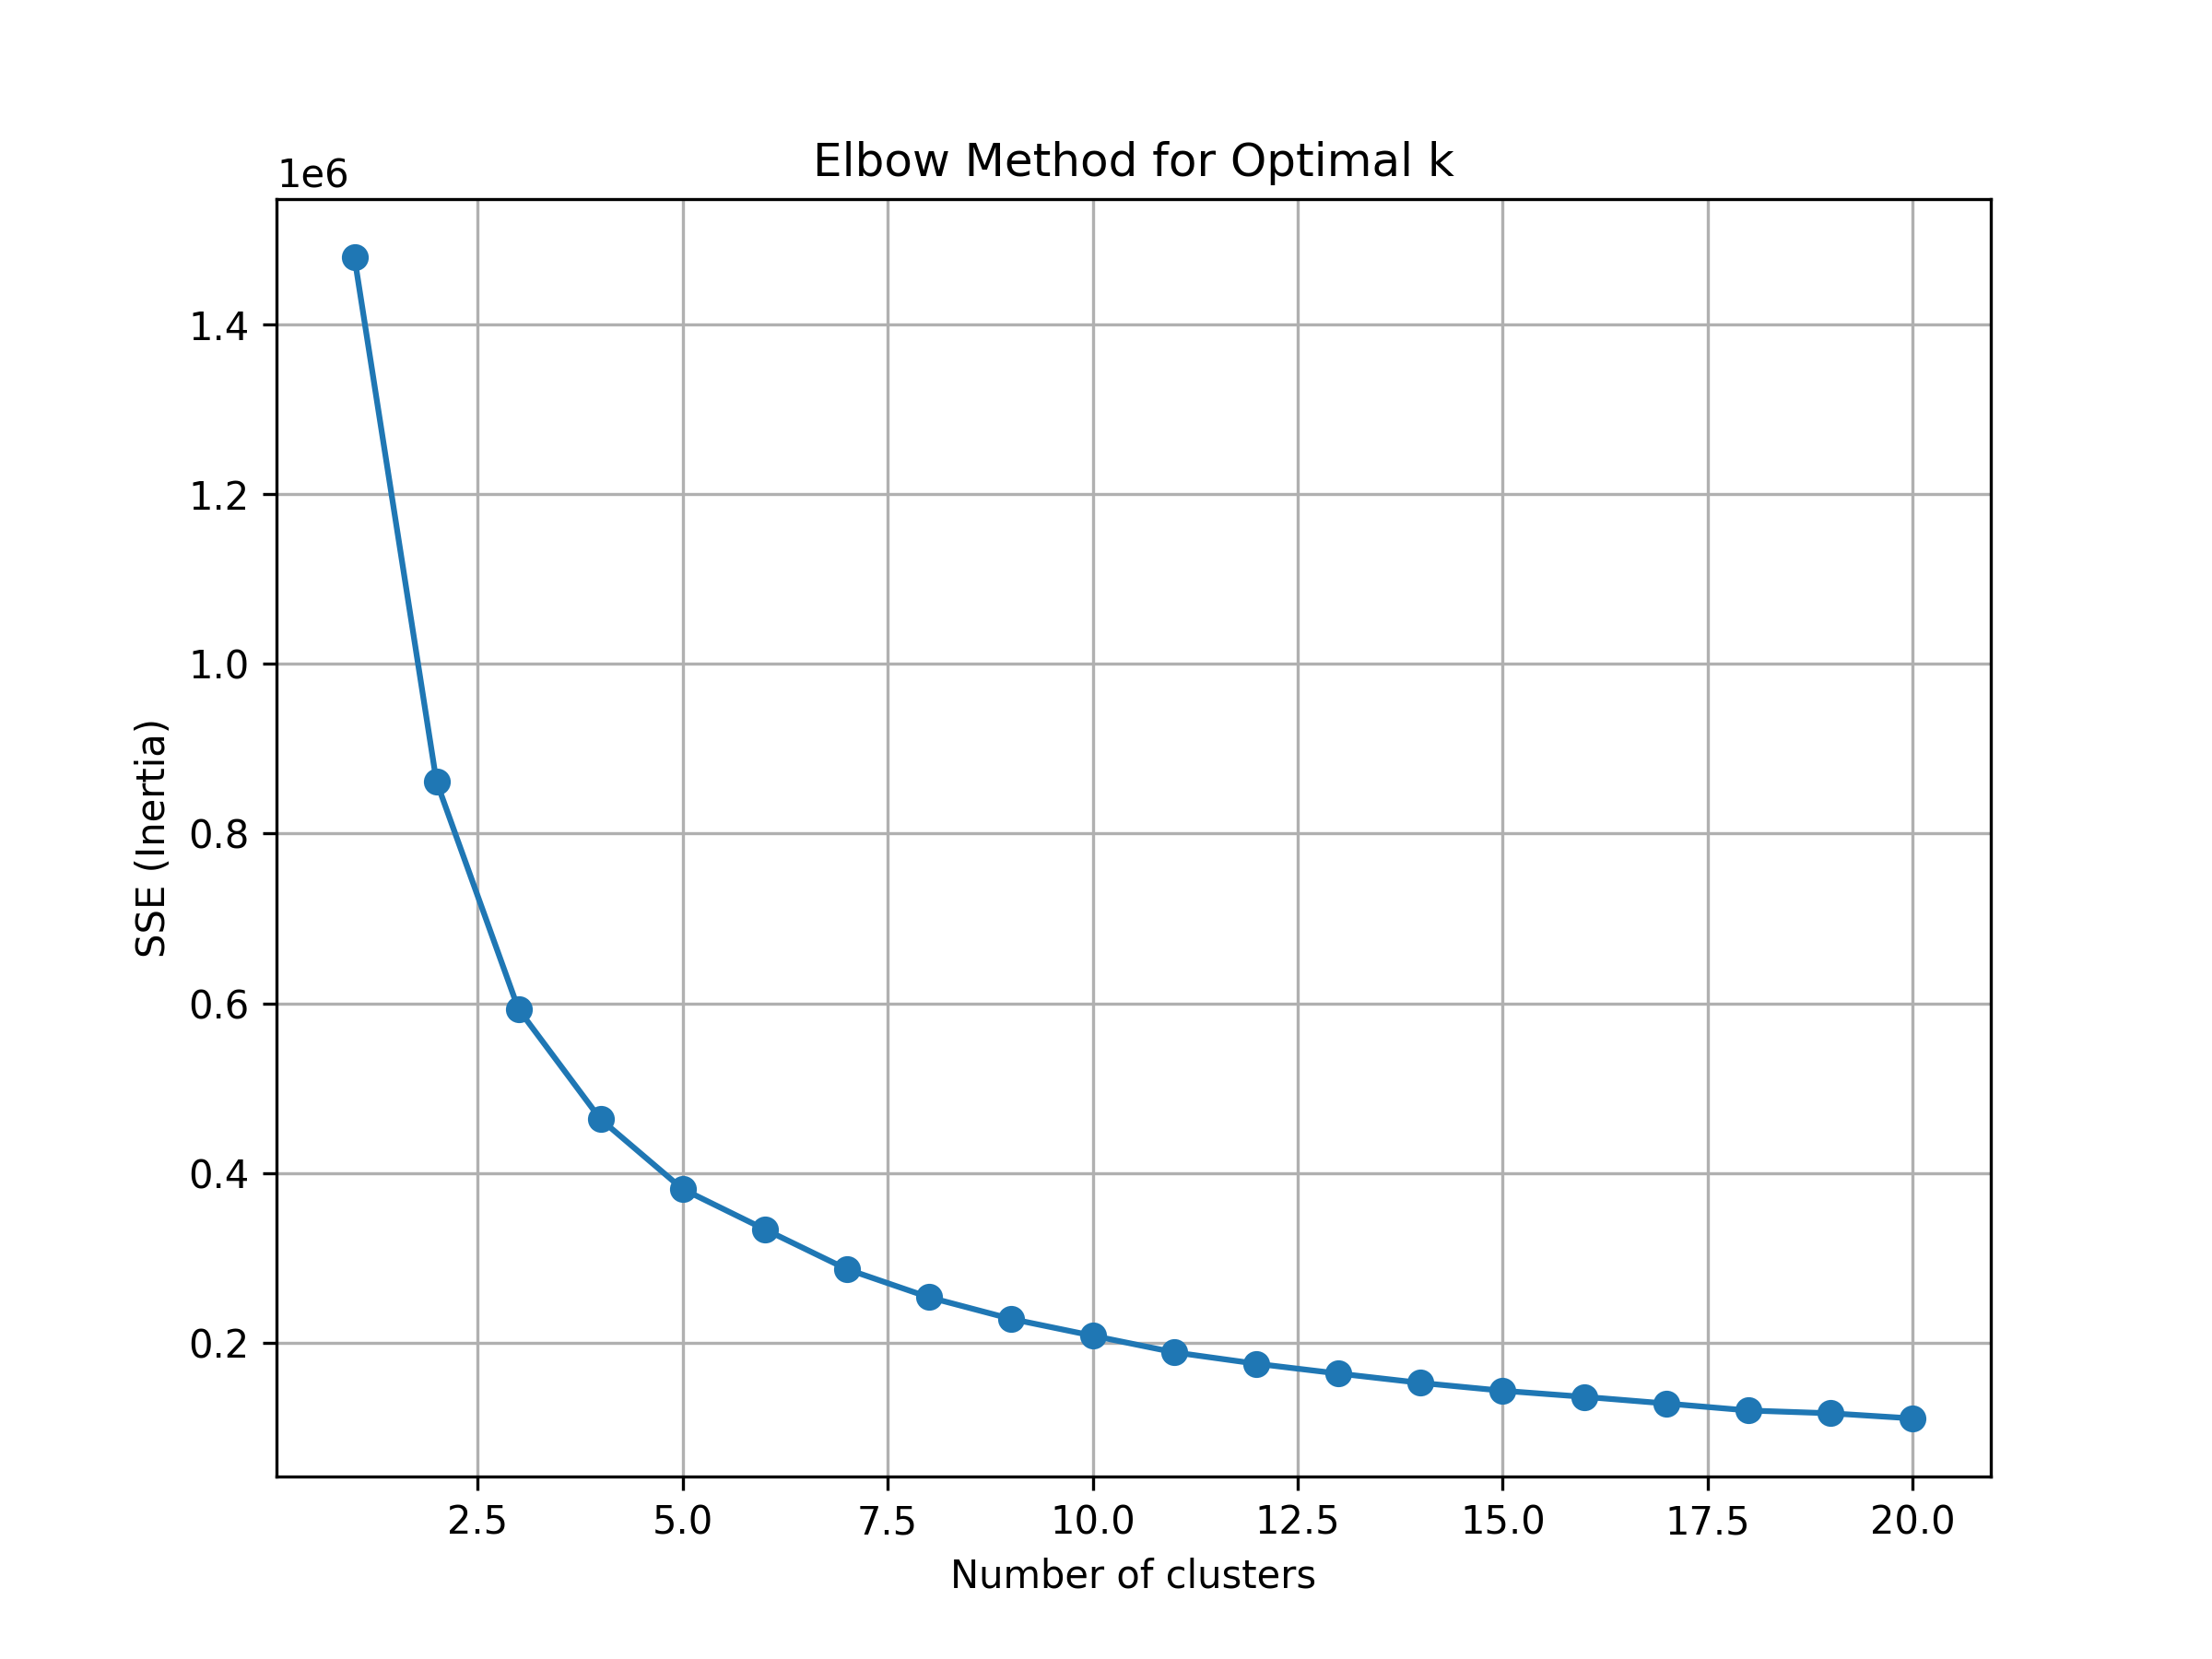
\includegraphics[width=0.7\columnwidth]{teoria/elbow_method.png} 
        \caption{Grafico rappresentante il metodo del gomito}
        \label{fig:gomito}
      \end{figure}
    \newpage
    \item Il Silhouette score indica quanto i punti appartenenti a un \emph{cluster} sono simili tra loro e quanto differiscono dai punti contenuti negli altri \emph{cluster}.
    Varia tra -1 e 1, se il valore è vicino a 1 il punto è all'interno del suo \emph{cluster} e ben separato dai \emph{cluster} limitrofi, se è vicino a 0 il punto è confinante tra due \emph{cluster} infine un valore negativo indica l'assegnazione a un \emph{cluster} sbagliato.
\end{itemize}

\section{PCA}
L'analisi dei componenti principali è un algoritmo non supervisionato in grado di estrarre le informazioni più rilevanti da \emph{\gls{dataset}} di grandi dimensioni, riducendo così la complessità del modello ed evitando che si presenti il fenomeno della "maledizione della dimensionalità"\footcite{site:PCA}.\\La maledizione della dimensionalità si verifica all'aumentare della dimensionalità dei dati: con l'aumentare delle dimensioni, il volume dello spazio aumenta in maniera esponenziale, rendendo difficile l'elaborazione da parte degli algoritmi di \emph{machine learning}, che dovranno lavorare su dati molto sparsi con conseguenze negative per le prestazioni.\\Tra gli ulteriori vantaggi che hanno portato all'adozione della PCA sono presenti la riduzione dei tempi di calcolo dovuta alla minor quantità di \emph{\gls{feature}} e la possibilità di visualizzare i risultati del \emph{clustering} su un grafico cartesiano bidimensionale (Fig.~\ref{fig:pca-chart}) aumentando il livello di comprensione dell'utente.

\begin{figure}[!h] 
    \centering 
    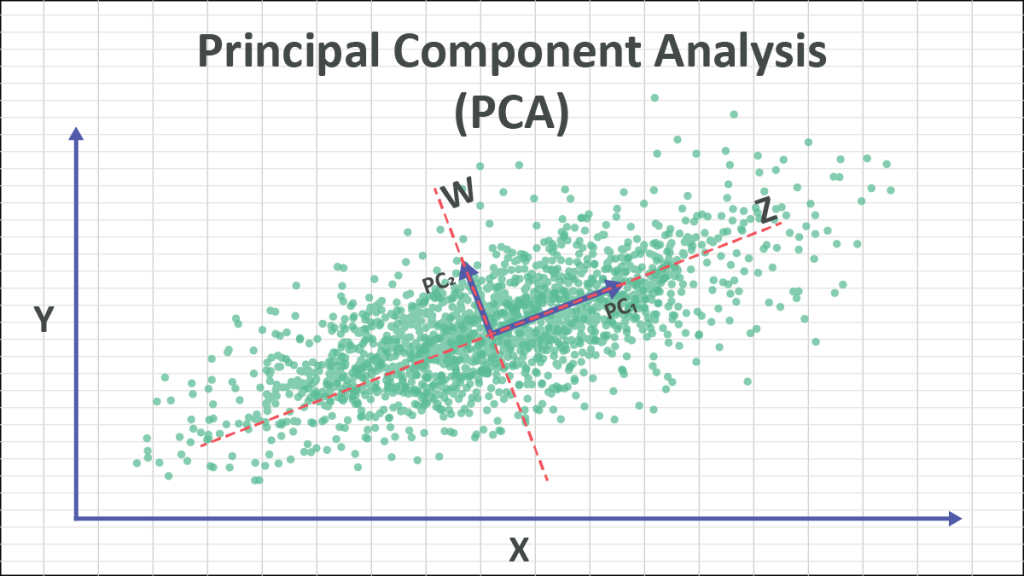
\includegraphics[width=0.7\columnwidth]{teoria/pca-chart.png} 
    \caption{Grafico contenente PCA}
    \label{fig:pca-chart}
  \end{figure}

\newpage

\section{Reti neurali}
Le reti neurali (Fig.~\ref{fig:rete-neurale}) sono un processo di \emph{machine learning} che sfrutta nodi interconnessi tra di loro (anche chiamati neuroni) in una struttura a strati ispirata al cervello umano (da qui \emph{neural network}).
In genere consistono di un sistema adattivo utilizzato dai computer per imparare dagli errori commessi e automigliorarsi\footcite{site:rete-neurale}.

\begin{figure}[!h] 
    \centering 
    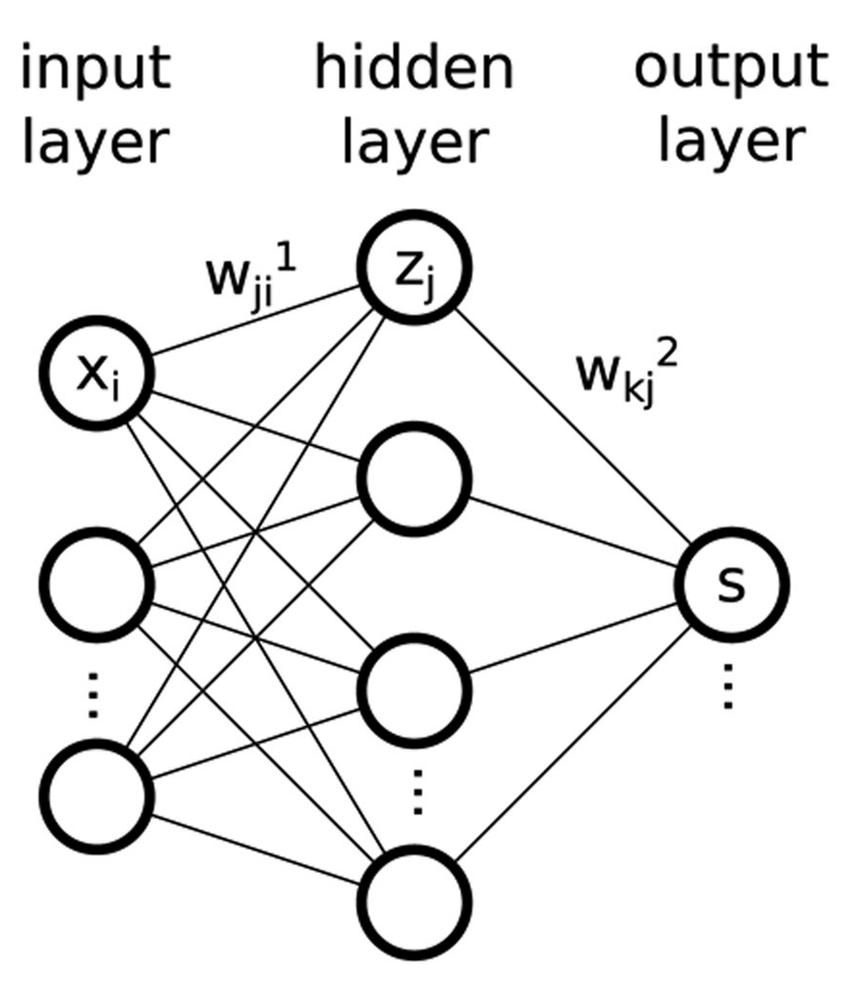
\includegraphics[width=0.4\columnwidth]{teoria/reteneurale.png} 
    \caption{Esempio di rete neurale}
    \label{fig:rete-neurale}
  \end{figure}

\subsubsection{Struttura}
All'interno di una rete neurale sono presenti:
\begin{itemize}
    \item \textbf{Input layer}: riceve l'\emph{input} che la rete deve elaborare.
    \item \textbf{Hidden layer}: possono essere uno o più e si occupano della elaborazione del dato in \emph{input}.
    \item \textbf{Output layer}: mostra l'\emph{output} dell'elaborazione.
\end{itemize}

\subsection{Apprendimento}
Gli strati densi (\emph{dense layer}) sono alla base della rete neurale e sono composti dai neuroni.
Ogni \emph{layer} è interconnesso con lo strato che lo precede e con quello successivo, in particolare ogni neurone dello strato è connesso a ogni neurone dello strato successivo.

\subsubsection{Funzionamento del neurone}

\begin{itemize}
    \item Ogni connessione ha un peso che indica la forza della connessione e il suo valore può essere positivo o negativo.
    \item L'\emph{input} che un neurone riceve da ciascuno dei neuroni a cui è connesso si calcola moltiplicando il segnale proveniente da quel neurone per il peso sulla connessione.
    \item L'\emph{input} totale del neurone è la sommatoria delle attivazioni che il neurone riceve dagli altri neuroni.
    \item Lo stato di attivazione finale viene calcolato attraverso una funzione di attivazione (ad esempio RELU o sigmoide, Fig.~\ref{fig:relu-sigmoid}).
    \item L'\emph{output} dei neuroni viene inviato ai neuroni successivi\footcite{LectureA}.
\end{itemize}
Lo schema successivo mostra il procedimento appena descritto (Fig.~\ref{fig:neurone})

\begin{figure}[!h] 
    \centering 
    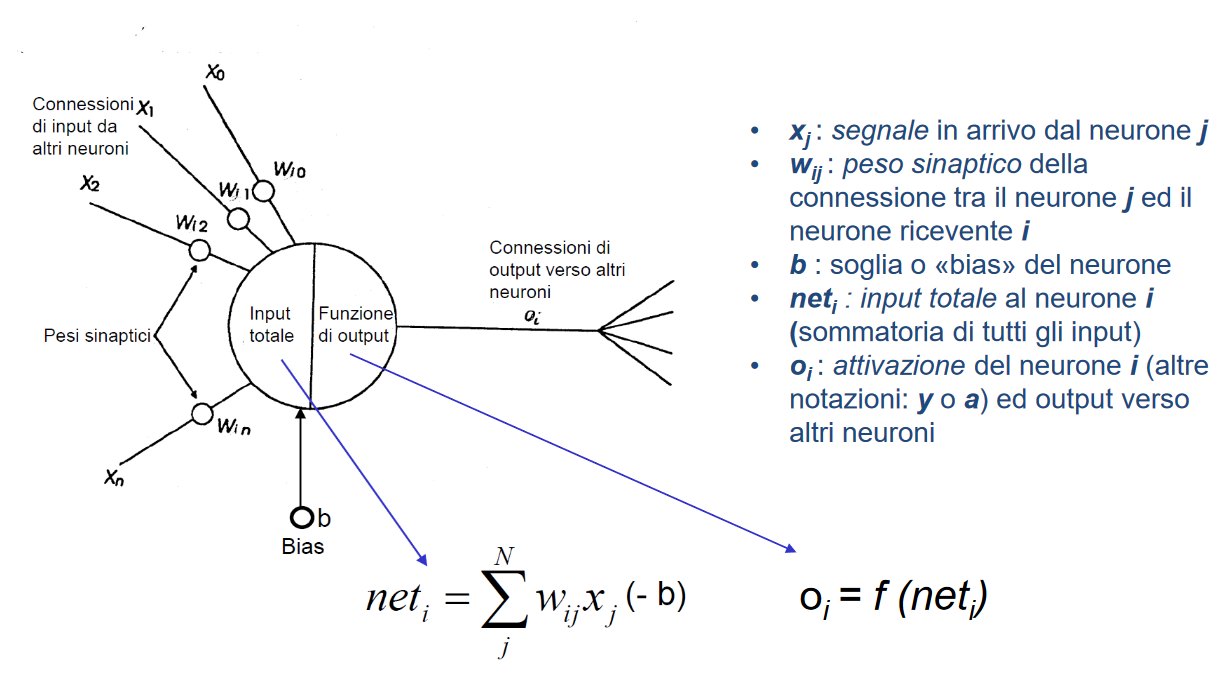
\includegraphics[width=0.9\columnwidth]{teoria/neurone.png} 
    \caption{Funzionamento del neurone}
    \label{fig:neurone}
  \end{figure}

  \begin{figure}[!h] 
    \centering 
    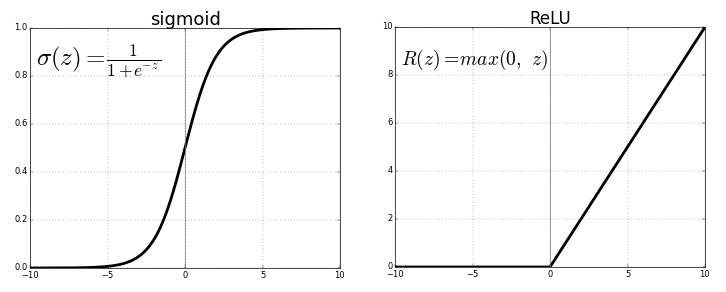
\includegraphics[width=0.8\columnwidth]{teoria/relu-sigmoid.png} 
    \caption{Funzioni di attivazione}
    \label{fig:relu-sigmoid}
  \end{figure}

\newpage

\subsubsection{Fasi di apprendimento} 
Inizialmente la rete riceve in \emph{input} il vettore, i pesi e i \emph{bias} vengono decisi in maniera casuale.
I dati si spostano di strato in strato fino a raggiungere quello di \emph{output} (\emph{forward propagation}, Fig.~\ref{fig:propagation}), successivamente la funzione di perdita misura il grado di errore e tramite la \emph{backward propagation} avviene l'Aggiornamento dei pesi.
Queste fasi vengono ripetute per un numero adeguato di volte (epoche) per ridurre man mano l'errore.

\begin{figure}[!h] 
    \centering 
    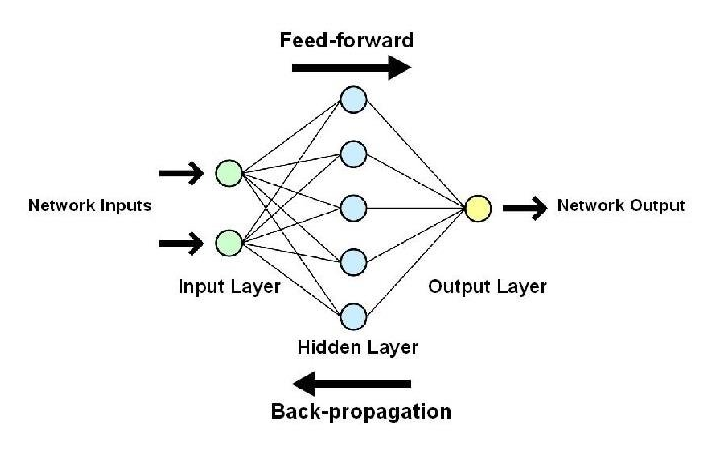
\includegraphics[width=0.6\columnwidth]{teoria/propagation.png} 
    \caption{Forward e backward propagation}
    \label{fig:propagation}
  \end{figure}


\subsection{Classificazione}
I dati da classificare vengono inseriti all'interno della rete neurale che fornisce in \emph{output} la classe di appartenenza di ciascun dato (Fig.~\ref{fig:classificazione}).

\begin{figure}[!h] 
    \centering 
    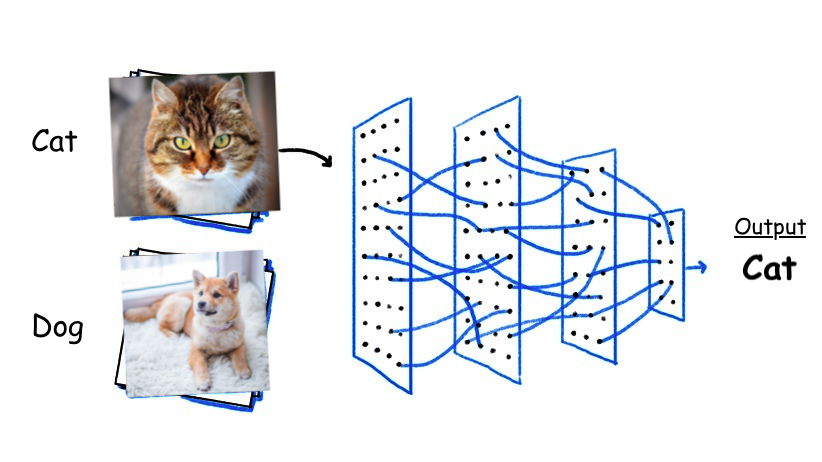
\includegraphics[width=0.6\columnwidth]{teoria/classificazione.png} 
    \caption{Classificazione dei dati}
    \label{fig:classificazione}
  \end{figure}

\newpage

\section{Deep learning}
Con il termine \emph{deep learning} si identificano reti neurali con un numero di strati nascosti maggiore o uguale a due (Fig.~\ref{fig:deep-learning}).

\begin{figure}[!h] 
    \centering 
    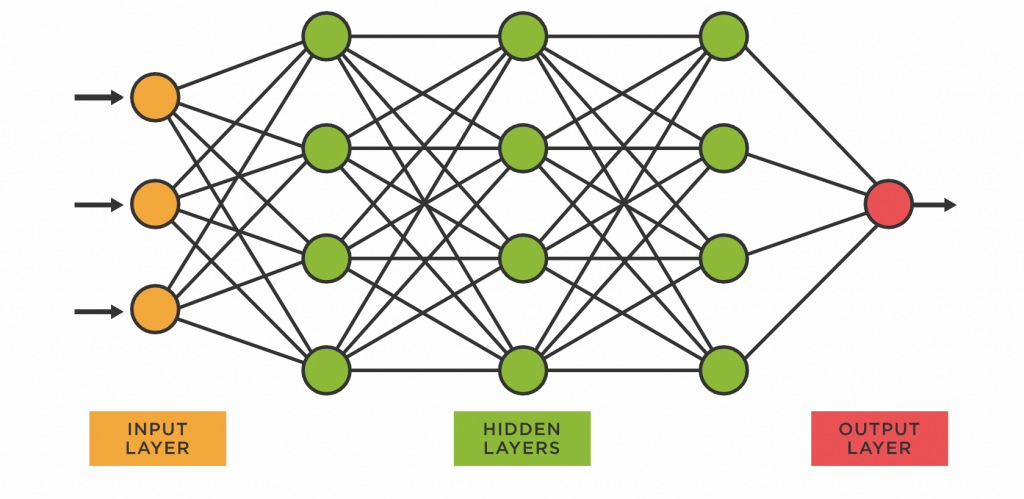
\includegraphics[width=0.8\columnwidth]{teoria/deep-learning.png} 
    \caption{Esempio di rete neurale con più strati nascosti}
    \label{fig:deep-learning}
  \end{figure}

\subsection{Convolutional neural network}
Le reti neurali convoluzionali (CNN, Fig.~\ref{fig:cnn}) sono un esempio di \emph{deep learning}, esse sfruttano dei \emph{layer} convoluzionali per eseguire la classificazione di dati tridimensionali, come ad esempio le classiche immagini raster.

\begin{figure}[!h] 
    \centering 
    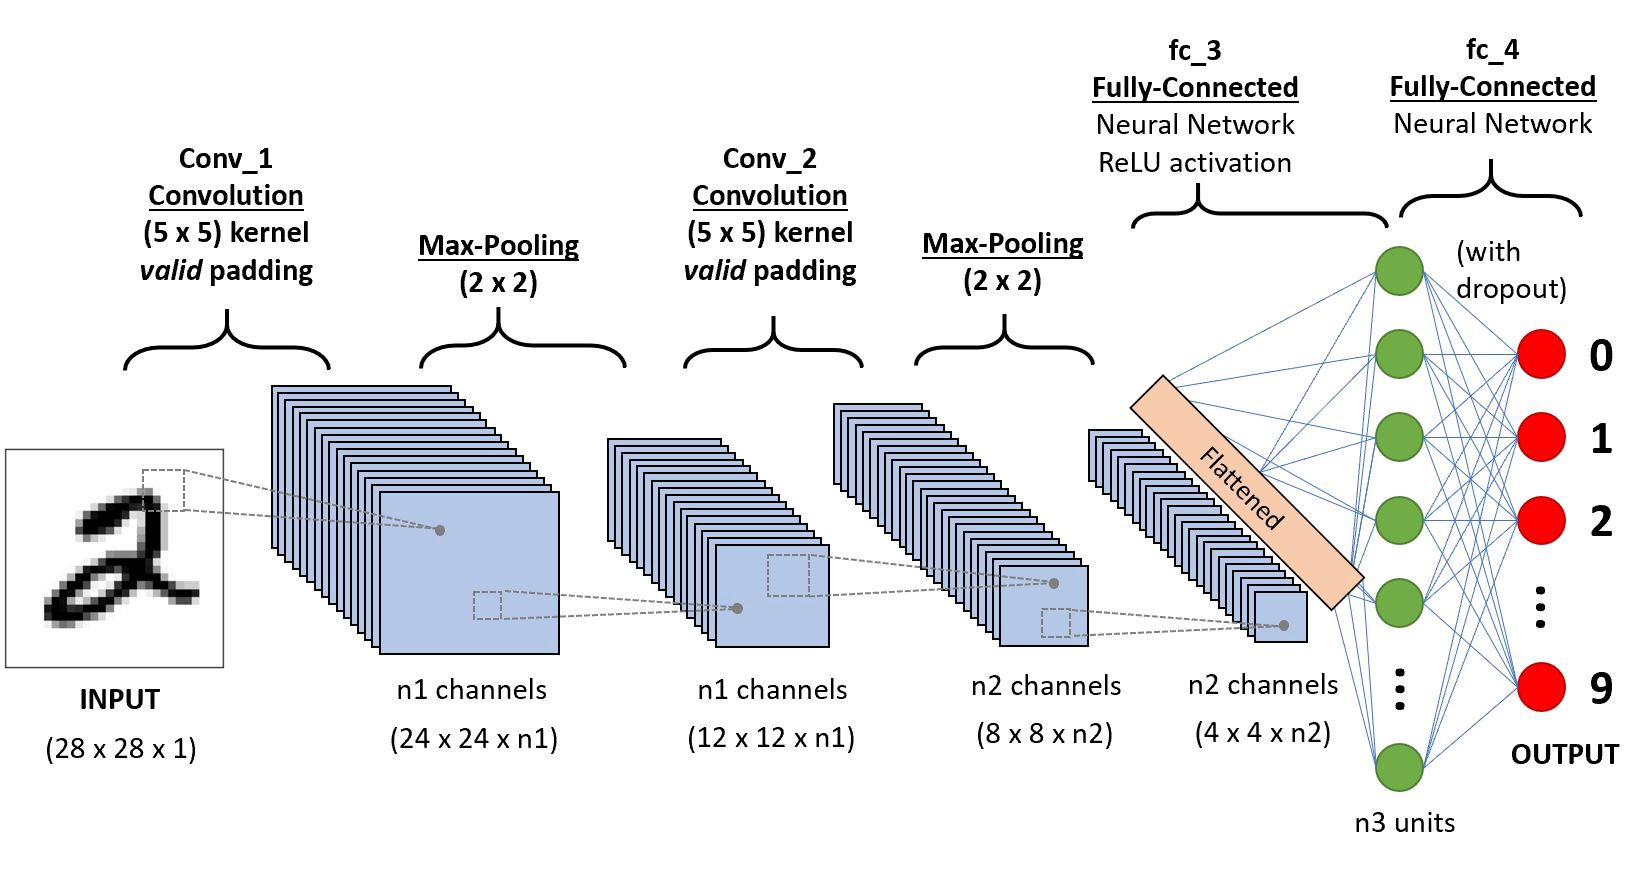
\includegraphics[width=0.8\columnwidth]{teoria/cnn.png} 
    \caption{Esempio di rete neurale convoluzionale}
    \label{fig:cnn}
  \end{figure}

\newpage

\subsubsection{Layer convoluzionali}
I \emph{layer} convoluzionali hanno come scopo l'estrazione di \emph{\gls{feature}} dalle immagini (texture, bordi, ecc...).
Per spiegare il funzionamento di un \emph{layer} convoluzionale è necessario introdurre la nozione di \emph{kernel}.\\Il \emph{kernel} (filtro, Fig.~\ref{fig:kernel}) è una matrice contenente dei pesi, che viene spostata lungo l'immagine effettuando una convoluzione in ogni posizione.

\begin{figure}[!h] 
    \centering 
    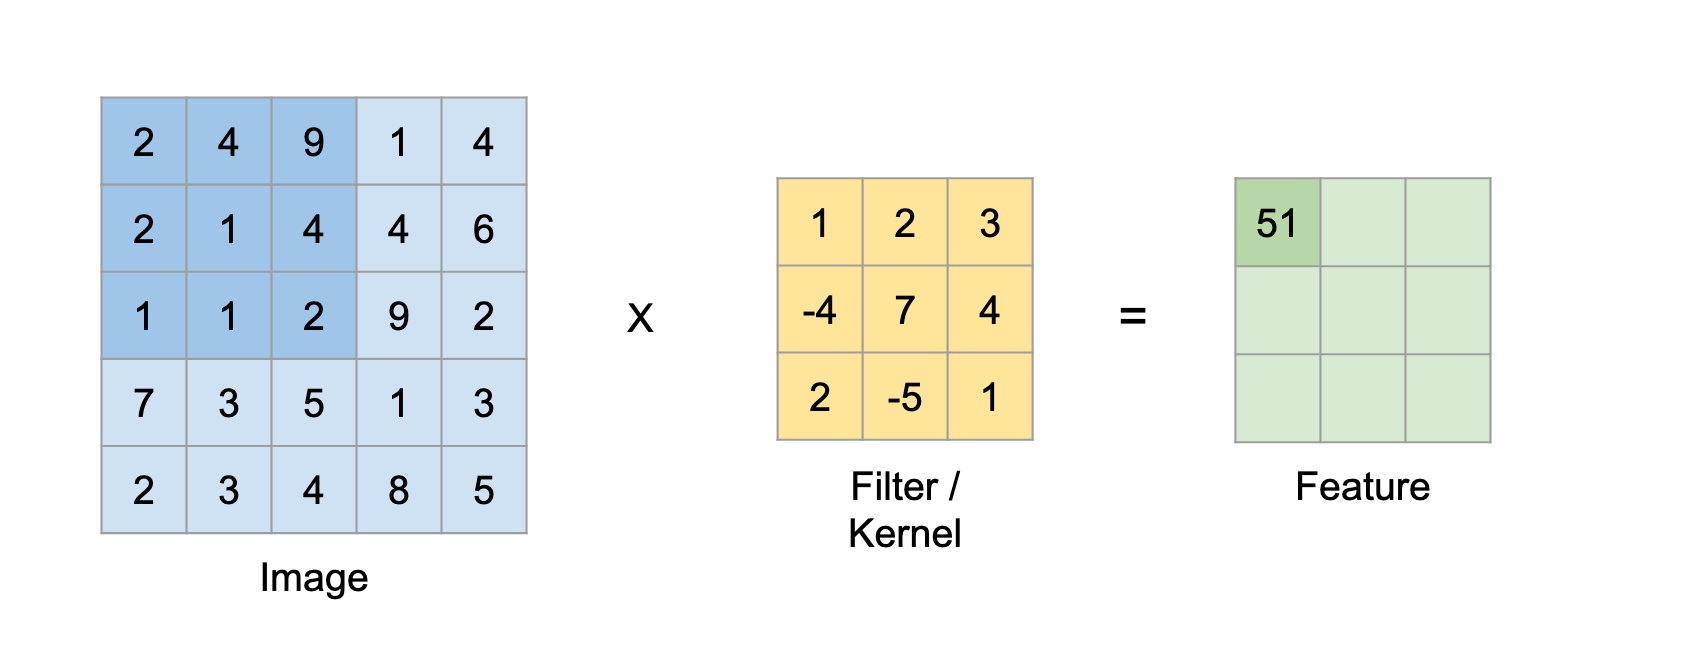
\includegraphics[width=0.8\columnwidth]{teoria/kernel.png} 
    \caption{Funzionamento del kernel}
    \label{fig:kernel}
  \end{figure}
Esempio con \emph{kernel} di dimensioni 3x3:

\begin{lstlisting}[language=Python, frame=none]
    [ -1,  0,  1 ]
    [ -1,  0,  1 ]
    [ -1,  0,  1 ]
\end{lstlisting}


\begin{enumerate}
    \item Posizionamento del filtro: il \emph{kernel} viene inserito sulla prima zona 3x3 dell'immagine.
    \item Moltiplicazione di ogni elemento: ogni peso presente nel \emph{kernel} viene moltiplicato per il valore corrispondente contenuto nella porzione di immagine.
    \newpage
    \begin{lstlisting}[language=Python, frame=none]
        PORZIONE DI IMMAGINE
        [ 10, 20, 30 ]
        [ 40, 50, 60 ]
        [ 70, 80, 90 ]

        PRODOTTO CON I PESI DEL KERNEL
        (-1 * 10) + (0 * 20) + (1 * 30) +
        (-1 * 40) + (0 * 50) + (1 * 60) +
        (-1 * 70) + (0 * 80) + (1 * 90)
            
    \end{lstlisting}
    \item \emph{Output} della convoluzione: tutti i risultati delle moltiplicazioni vengono sommati tra di loro e il valore ottenuto viene posizionato nella \emph{feature map} nel punto che corrisponde alla regione dell'immagine elaborata.
    \begin{lstlisting}[language=Python, frame=none]
        (-10) + (0) + (30) +
        (-40) + (0) + (60) +
        (-70) + (0) + (90) = 60
    \end{lstlisting}
    \item Riposizionamento del filtro: il \emph{kernel} viene riposizionato spostandolo di uno o più pixel (\emph{stride}) e il flusso si ripete fino alla copertura completa dell'immagine.
\end{enumerate}
L'otuput del \emph{layer} convoluzionale è una serie di \emph{feature map} ognuna corrispondente a ciascun filtro.

\begin{lstlisting}[language=Python, frame=none]
    conv_layer= Conv2D(32, (3, 3), activation='relu', padding='same')(input_img)
\end{lstlisting}

\begin{itemize}
    \item 32 rappresenta il numero di filtri.
    \item (3,3) rappresenta la dimensione dei \emph{kernel}.
    \item activation='relu' indica che come funzione di attivazione verrà utilizzata relu.
    \item padding='same' consente di mantenere la dimensione dell'immagine in \emph{input} anche dopo l'applicazione dei filtri
\end{itemize}


\subsubsection{Layer di pooling}
I \emph{layer} di \emph{pooling} (Fig.~\ref{fig:pooling}) servono per ridurre le dimensioni delle \emph{feature map} mantenendo le caratteristiche importanti e riducendo di conseguenza la complessità di calcolo.


\begin{figure}[!h] 
    \centering 
    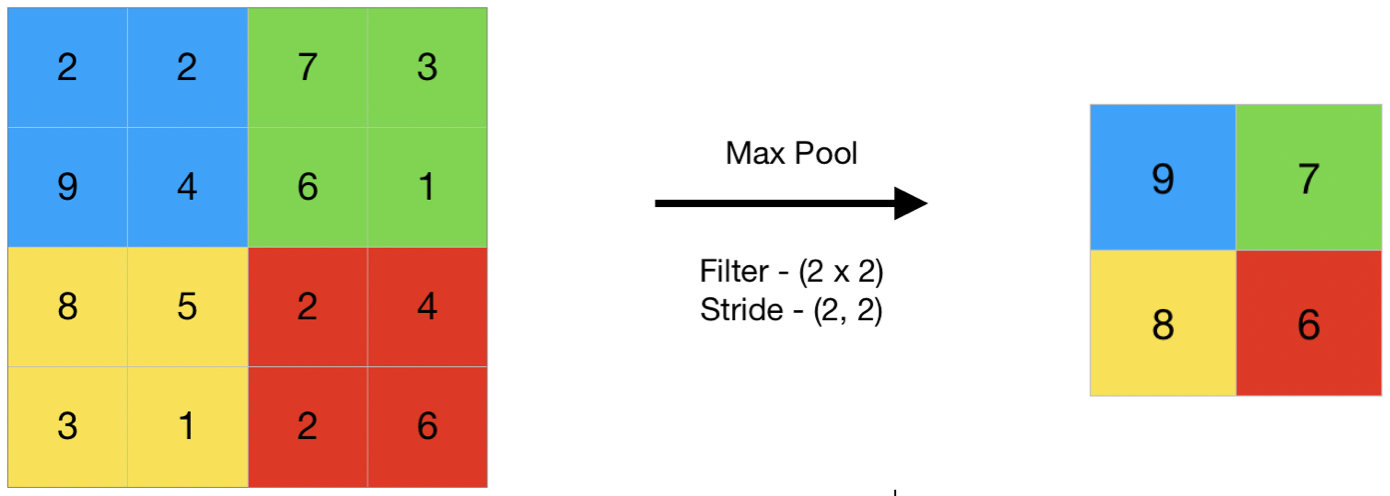
\includegraphics[width=0.8\columnwidth]{teoria/pooling.png} 
    \caption{Funzionamento del pooling}
    \label{fig:pooling}
  \end{figure}



\subsubsection{Funzionamento di un layer di pooling}
Esempio di \emph{Max pooling} con matrici 2x2 e \emph{stride} di 2 pixel


\begin{lstlisting}[language=Python, frame=none]
    FEATURE MAP 4x4
    [ 1, 3, 2, 4 ]
    [ 5, 6, 8, 7 ]
    [ 3, 2, 1, 0 ]
    [ 1, 2, 4, 3 ]
\end{lstlisting}

\begin{enumerate}
    \item Divisione della \emph{feature map} in matrici 2x2:
    \begin{lstlisting}[language=Python, frame=none]
    
        [ 1, 3 ]
        [ 5, 6 ]
        
        [ 2, 4 ]
        [ 8, 7 ]
        
        [ 3, 2 ]
        [ 1, 2 ]
        
        [ 1, 0 ]
        [ 4, 3 ]

    \end{lstlisting}
    \item Calcolo del valore massimo per ogni matrice:
    
    \begin{lstlisting}[language=Python, frame=none]
        max(1, 3, 5, 6) = 6
        max(2, 4, 8, 7) = 8
        max(3, 2, 1, 0) = 3
        max(1, 2, 4, 3) = 4
    \end{lstlisting}

    \item Creazione di una nuova \emph{feature map} contenente i valori massimi:
    \begin{lstlisting}[language=Python, frame=none]
        [ 6, 8 ]
        [ 3, 4 ]
    \end{lstlisting}
\end{enumerate}
L'\emph{output} del \emph{layer} di \emph{pooling} in questo caso è una \emph{feature map} ridotta da 4x4 a 2x2.

\begin{lstlisting}[language=Python, frame=none]
    MaxPooling2D((2, 2), padding='same')(x)
\end{lstlisting}

\newpage

\section{Autoencoder}
L'\emph{auoencoder} (Fig.~\ref{fig:autoencoder-teoria}) è un \emph{neural network} in grado di comprimere il suo \emph{input} e di ricostruirlo in maniera similare come \emph{output}. \footcite[p.~499]{Goodfellow-et-al-2016}.

\begin{figure}[!h] 
    \centering 
    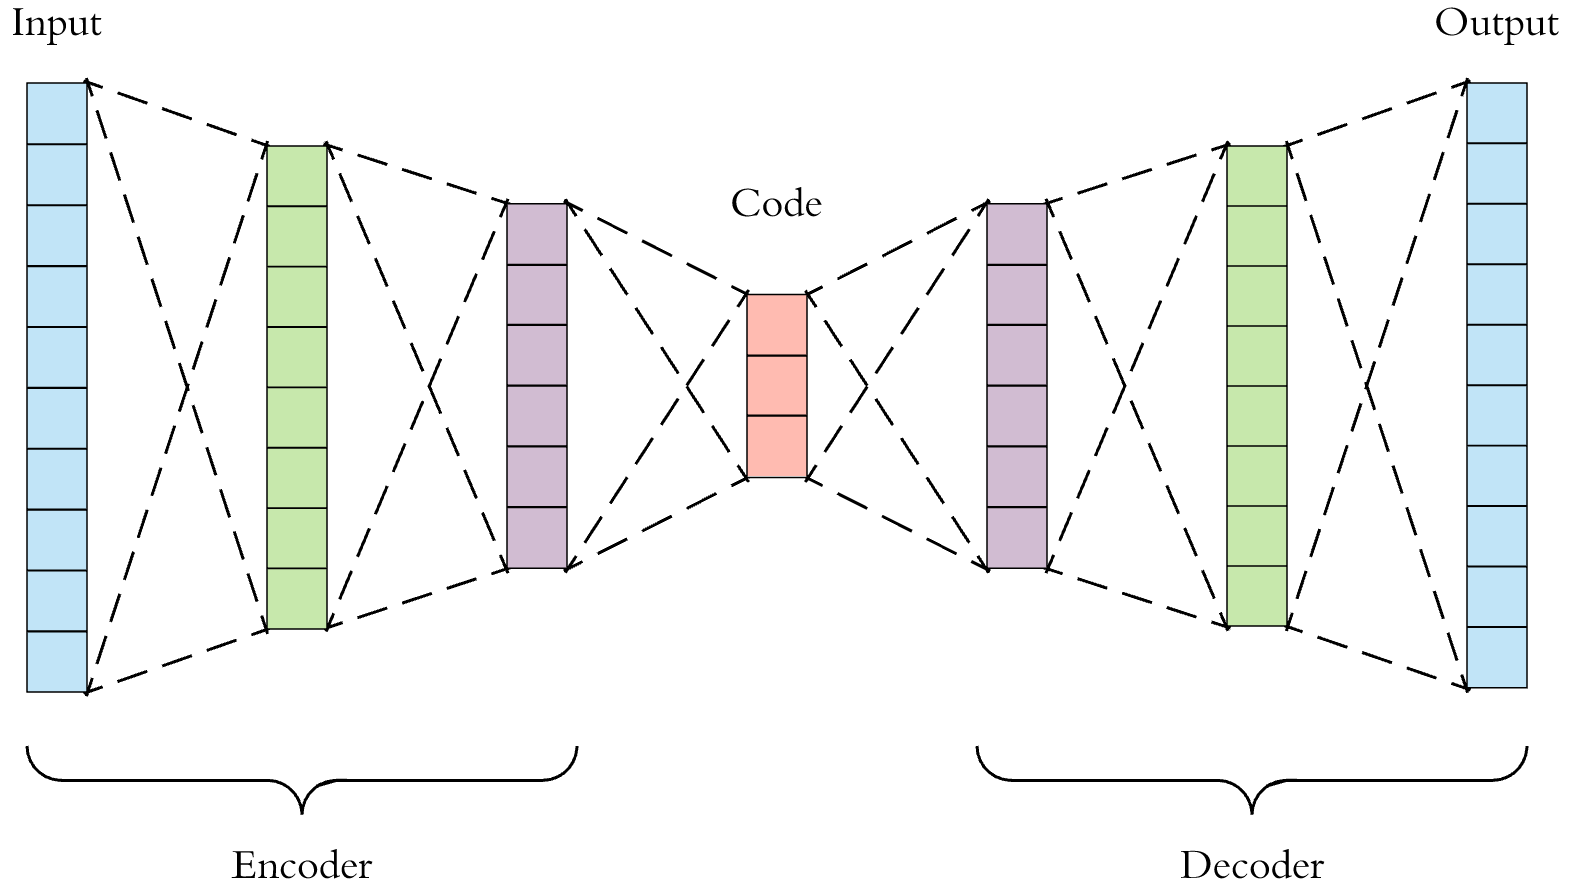
\includegraphics[width=0.7\columnwidth]{teoria/autoencoder.png} 
    \caption{Schema generale di un autoencoder}
    \label{fig:autoencoder-teoria}
  \end{figure}
L'architettura si compone di due parti principali:
\begin{enumerate}
    \item \textbf{Encoder}: comprime l'\emph{input} riducendolo di dimensionalità (codifica).
    \item \textbf{Decoder}: ricostruisce l'\emph{input} inziale partendo dalla codifica fatta dall'\emph{encoder}
\end{enumerate}
Il \emph{bottleneck} o \emph{latent space} contiene la codifica e sta nel mezzo delle due componenti; è il punto di arrivo del \emph{encoder} e la partenza del \emph{decoder}.

\subsection{Funzionamento}
\begin{enumerate}
    \item L'\emph{encoder} riceve un \emph{input} \( x \) e lo codifica creando una funzione \( z= f(x) \)
    \item Il \emph{bottleneck} contiene la codifica \( z \)
    \item Il \emph{decoder} cerca di decodificare \( z \) tramite la funzione \( g \) ottenendo come \emph{output} \( \hat{x} = g(z) \).
\end{enumerate}
Il processo di apprendimento ha come obiettivo minimizzare la loss function che misura la differenza tra \emph{input} iniziale e \emph{output} ricostruito dal \emph{decoder}.
\[ L(x, \hat{x}) = ||x - \hat{x}||^2 \]
Nell'esempio viene utilizzata la \emph{MSE (Mean Squared Error)}.
Ai fini del progetto la parte interessante dell'\emph{auoencoder} è proprio l'\emph{encoder} poiché comprime l'immagine in \emph{input} lasciando un set di \emph{\gls{feature}} nel \emph{bottleneck}; che possono essere utilizzate successivamente per il \emph{clustering}.









    \chapter{Progettazione e codifica}

\label{cap:progettazione}

\intro{Durante la fase di progettazione viene definita l'architettura del software, questa operazione consiste nella suddivisione del sistema in componenti distinti, ognuno con compiti differenti.
L'obiettivo è pianificare in maniera chiara tutte le azioni che l'applicativo dovrà svolgere prima di passare effettivamente alla codifica.}

\section{Architettura}
L'architettura (Fig.~\ref{fig:schema-architettura}) pensata prevede l'utilizzo di 4 componenti principali che si occupano di:
\begin{enumerate}
    \item Acquisire gli screenshot.
    \item Effettuare il clustering degli screenshot acquisiti.
    \item Valutare i siti web.
    \item Inviare e-mail promozionali.
\end{enumerate}
La suddivisione in componenti consente di avere un codice più strutturato e specializzato nell'assolvimento di determinati compiti; rende anche la comprensione da parte di altri programmatori più rapida e chiara.
I vari moduli comunicano con il database di SalesCRM attraverso l'utilizzo di API che eseguono interrogazioni e inserimenti.
Nel caso della comunicazione tra il modulo di clustering e quello di valutazione la condivisione di dati avviene in maniera diretta utilizzando la memoria dello stesso PC; questa modalità non si rivela problematica poiché garantisce uno scambio rapido di informazioni che deve essere svolto solo ed esclusivamente in fase di addestramento.

\begin{figure}[!h] 
    \centering 
    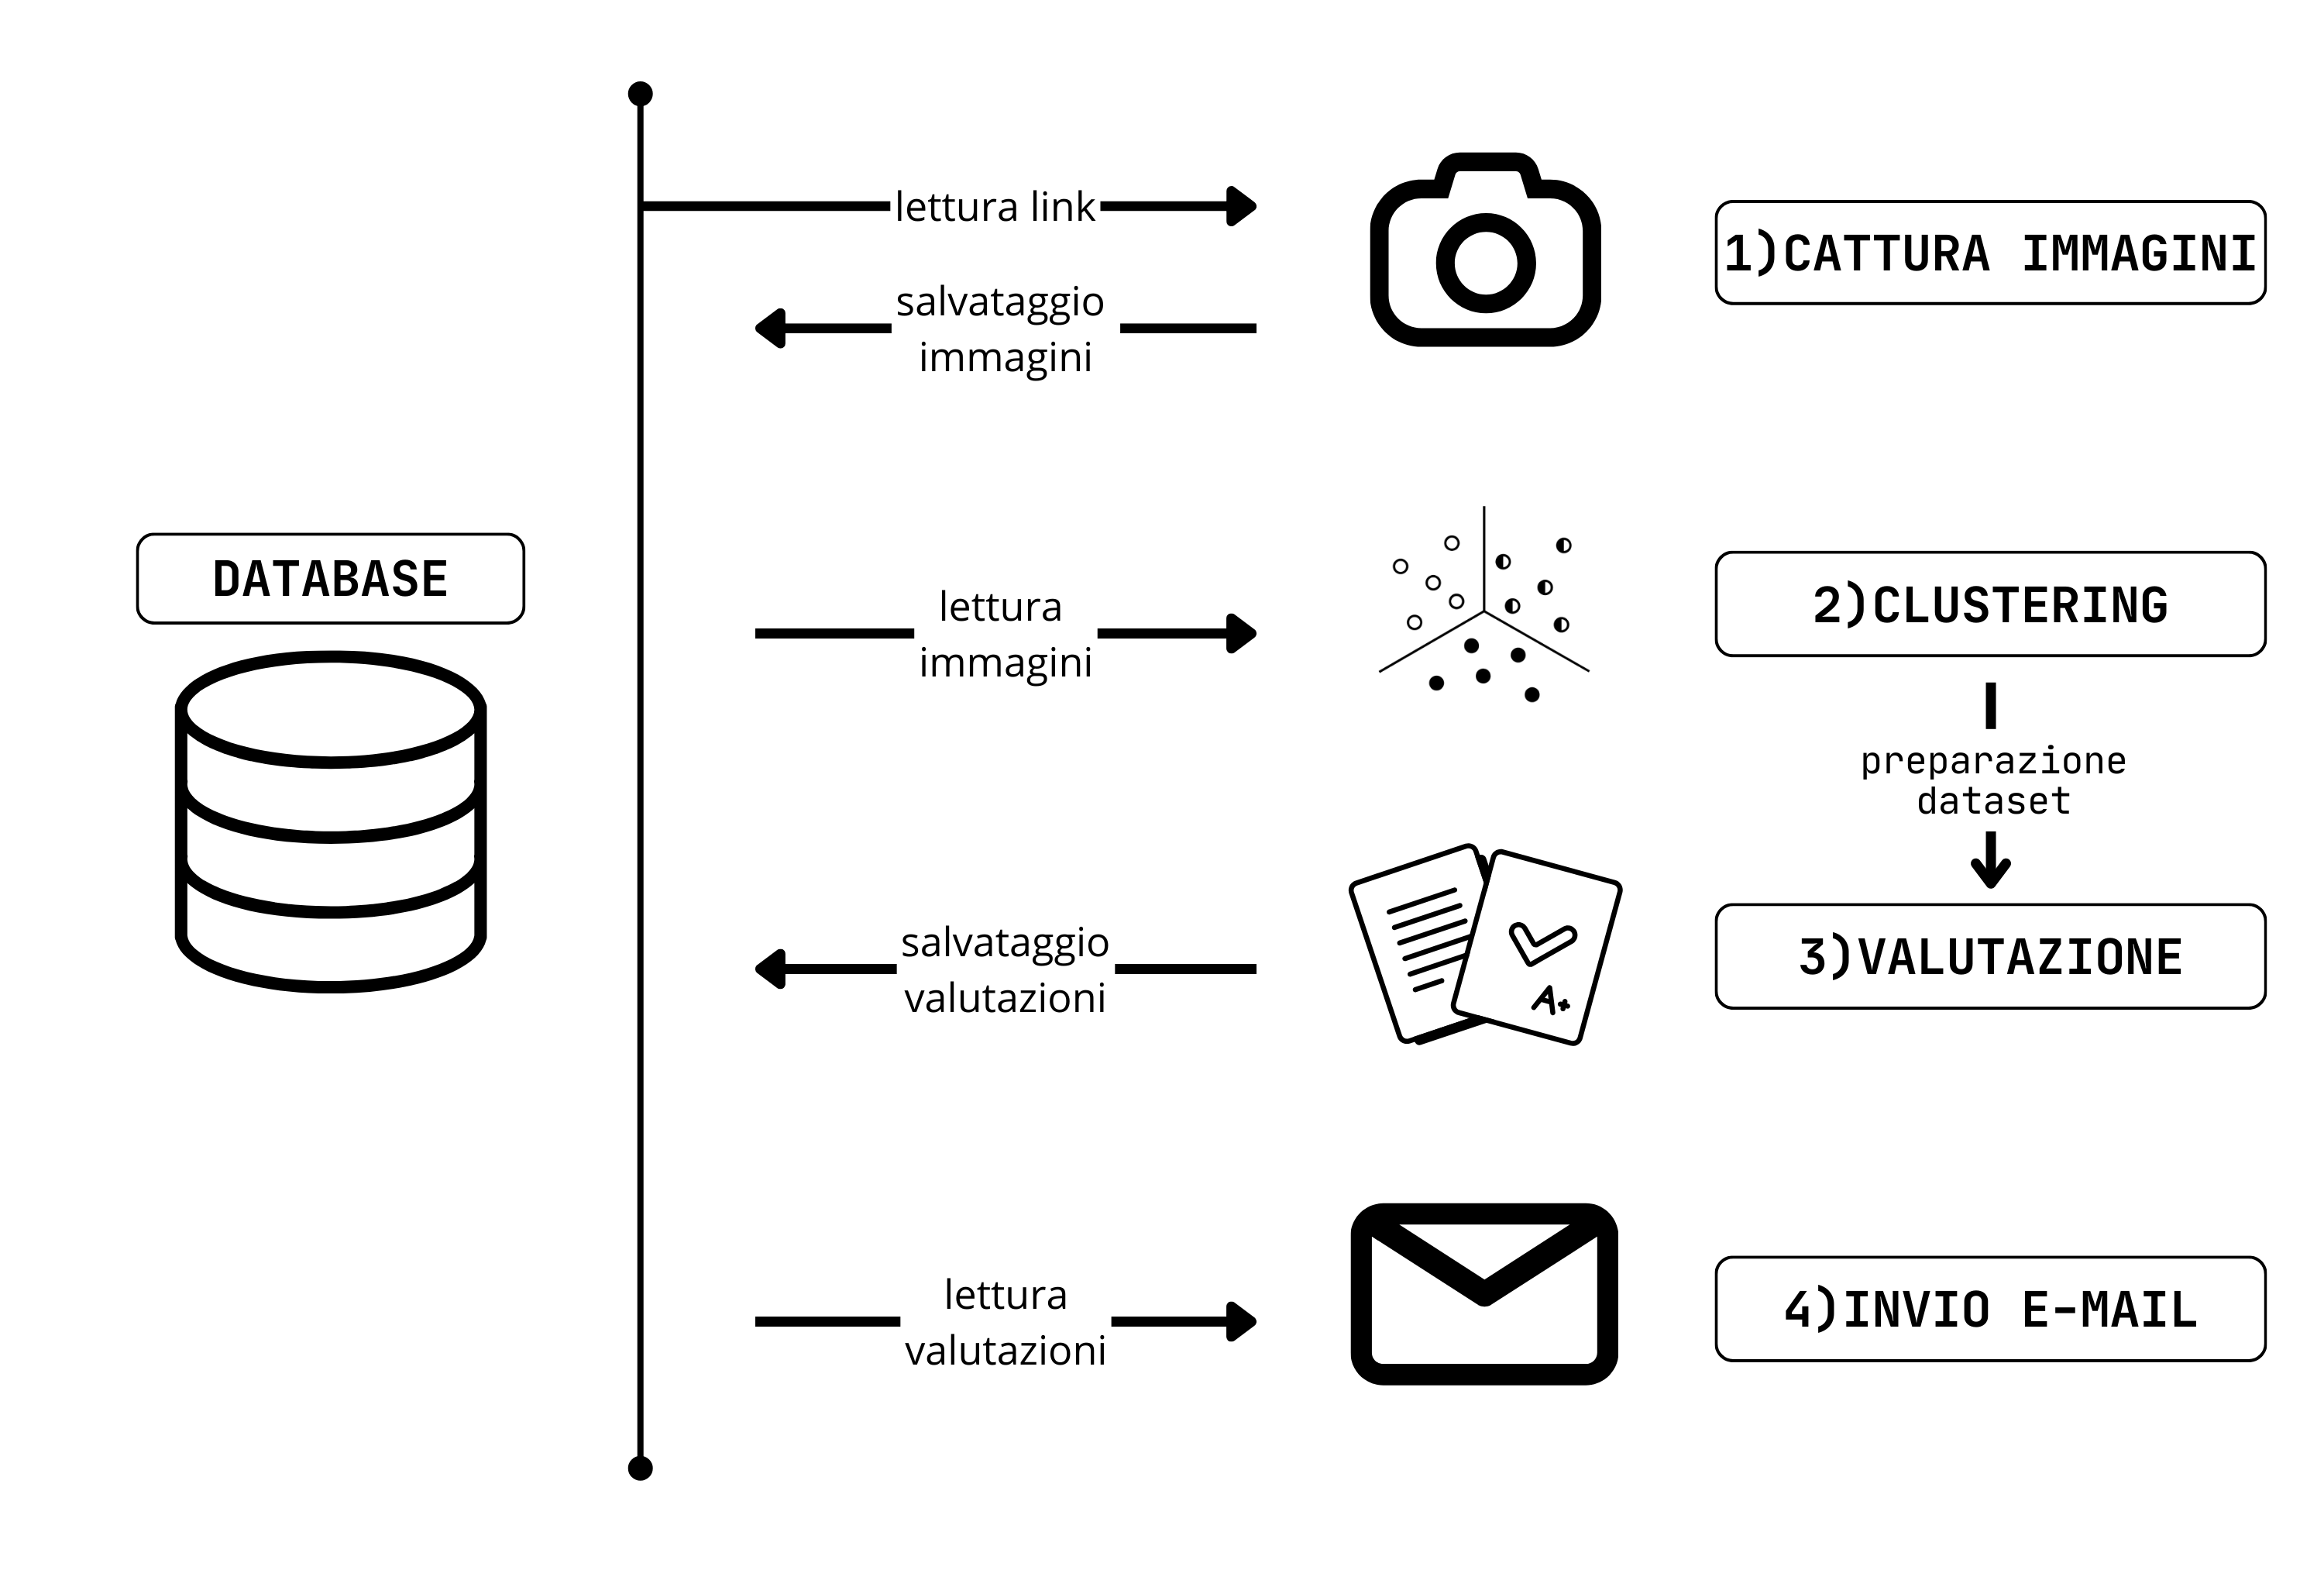
\includegraphics[width=0.9\columnwidth]{progettazione/schema-architettura.png} 
    \caption{Schema architetturale del progetto}
    \label{fig:schema-architettura}
  \end{figure}


\newpage

\section{Cattura immagini}
La prima fase del workflow (Fig.~\ref{fig:schema-cattura}) è composta da uno script Python che usufruisce della libreria Pyppeteer per acquisire gli screenshot dei siti contenuti nel database.
Più precisamente un web-scraper già implementato raccoglie i link delle pagine web dei clienti potenziali, successivamente li carica nel database di SalesCRM, dove verranno infine letti dallo script.
Per funzionare Pyppeteer necessita di chromium, dopo aver effettuato il controllo per verificare se esso sia presente o meno procede con la lettura dei link. 
L'automazione apre ogni indirizzo, aspetta qualche secondo e scatta uno screenshot. 
Tutte le immagini vengono poi convertite in formato Base64 per adattarsi alle tabelle già esistenti e salvate nel database.

\begin{figure}[!h] 
  \centering 
  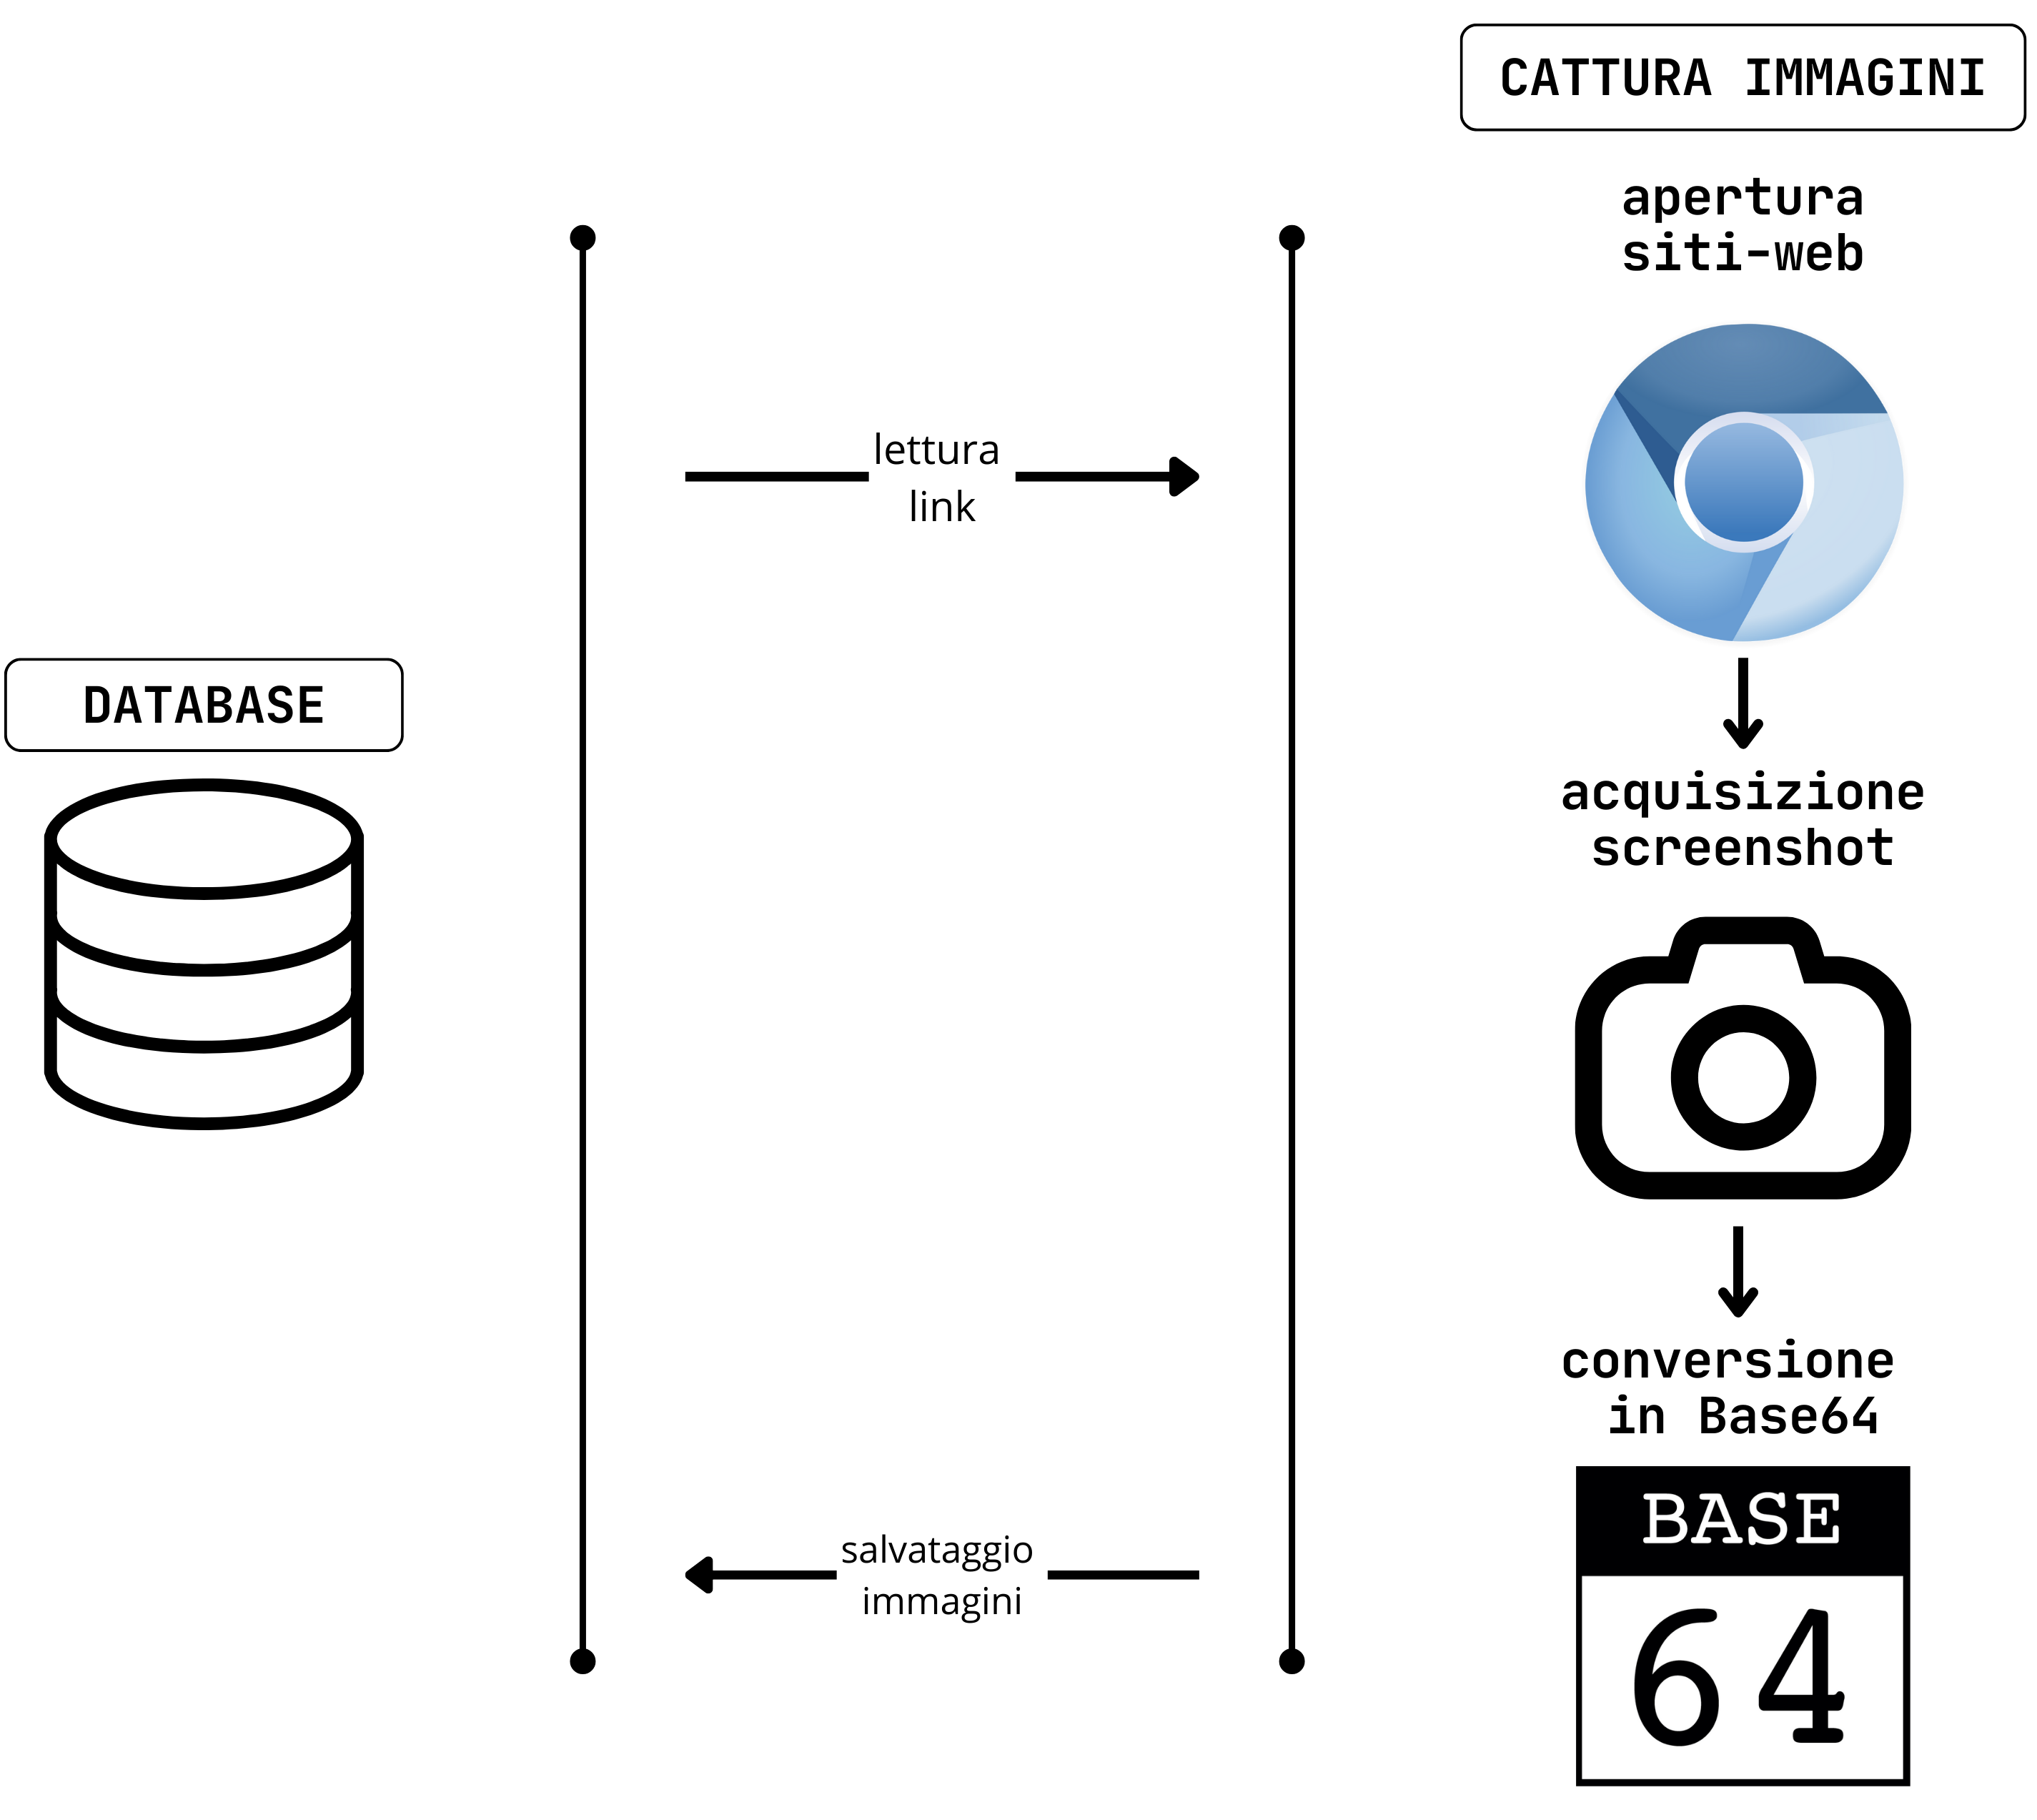
\includegraphics[width=0.5\columnwidth]{progettazione/schema-cattura.png} 
  \caption{Schema della fase di cattura}
  \label{fig:schema-cattura}
\end{figure}

\newpage

\section{Studio preliminare per l'estrazione delle feature}
L'estrazione delle feature è una fase fondamentale e necessita pertanto di uno studio più approfondito.

\subsection{Tentativi con autoencoder}
Gli autoencoder sono stati utilizzati inizialmente poiché si pensava che la soluzione migliore fosse la creazione di un modello CNN che si adattasse completamente alle feature presenti nei siti web, ma si è rivelato particolarmente difficile per i motivi seguenti:
\begin{itemize}
  \item Numero elevato di epoche di addestramento.
  \item Studio della quantità e tipologia degli strati.
  \item Bilanciamento arduo tra dimensioni accettabili e memoria a disposizione.
\end{itemize}

\subsubsection{Autoencoder con soli strati densi}
Il primo tentativo è stato effettuato utilizzando un autoencoder che sfrutta esclusivamente layer densi (Fig.~\ref{fig:schema-denso}), questo metodo nonostante abbia portato a dei risultati si è rivelato problematico visto che per funzionare in maniera efficiente, senza richiedere una GPU troppo prestante, necessita di immagini in bianco e nero di dimensioni ridotte a 128*128 (Fig.~\ref{fig:dense-ricostruita}).

\begin{figure}[!h] 
  \centering 
  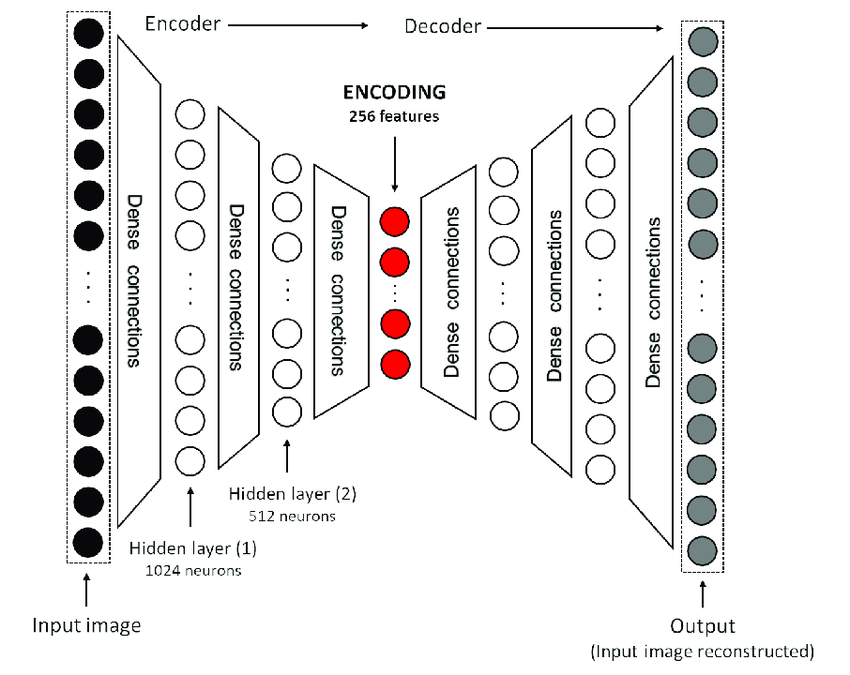
\includegraphics[width=0.6\columnwidth]{progettazione/autencoder_dense_layers.png} 
  \caption{Autoencoder con strati densi}
  \label{fig:schema-denso}
\end{figure}


\begin{figure}[!h] 
  \centering 
  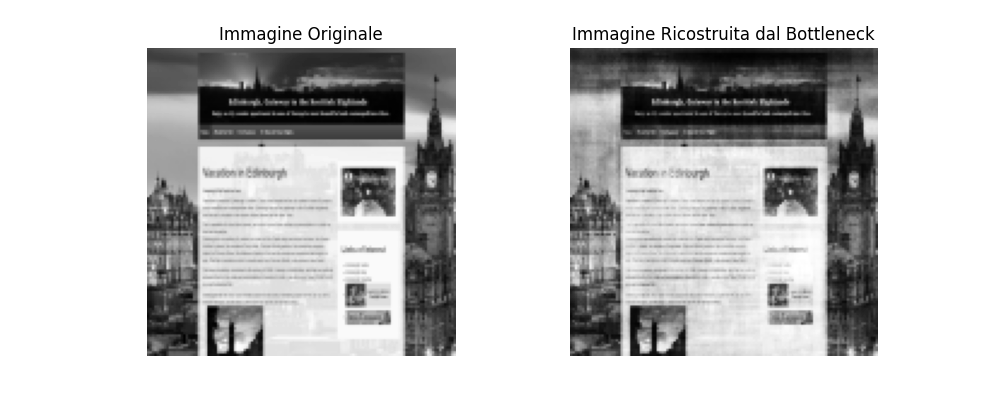
\includegraphics[width=1\columnwidth]{progettazione/dense_200Immagini_150Epoche_10BatchSize_BW.png} 
  \caption{Ricostruzione immagine ottenuta dal bottleneck dell'autoencoder a strati densi con 150 epoche di addestramento}
  \label{fig:dense-ricostruita}
\end{figure}

\newpage

\subsubsection{Autoencoder con strati convoluzionali}
L'autoencoder con strati convoluzionali (Fig.~\ref{fig:schema-conv}) ha consentito un netto miglioramento delle prestazioni e un consumo inferiore della memoria tali da poter aumentare le dimensioni delle immagini e implementare nuovamente l'utilizzo del colore.
Le modifiche non sono state comunque sufficienti per avere un esperienza di utilizzo solida.
Viene sotto riportata un immagine in bianco e nero di dimensioni 256*256 ottenuta dal bottleneck dell'autoencoder per comparare con il modello precedente (Fig.~\ref{fig:conv-ricostruita}).

\begin{figure}[!h] 
  \centering 
  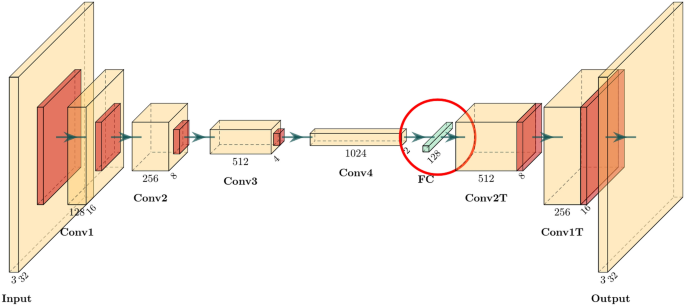
\includegraphics[width=0.7\columnwidth]{progettazione/Convolutional_autoencoder.png} 
  \caption{Autoencoder con strati convoluzionali}
  \label{fig:schema-conv}
\end{figure}


\begin{figure}[!h] 
  \centering 
  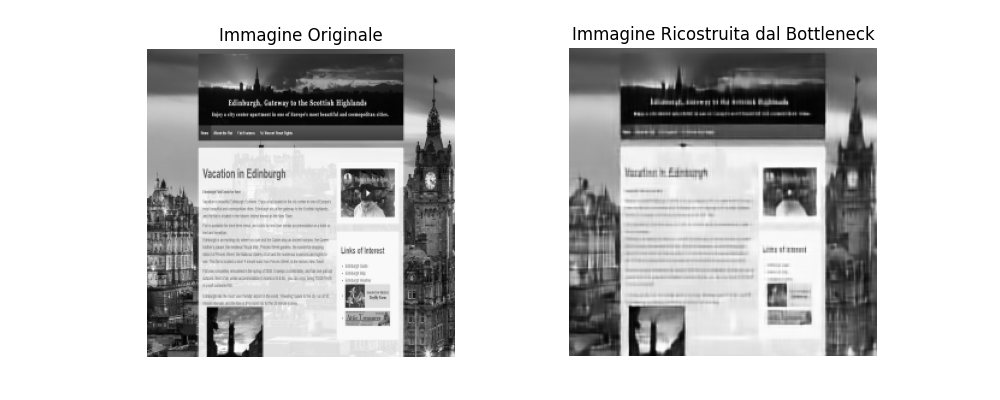
\includegraphics[width=1\columnwidth]{progettazione/Conv_BW_img_dim256Epochs500Batch32Images5000.png} 
  \caption{Ricostruzione immagine ottenuta dal bottleneck dell'autoencoder convoluzionale con 500 epoche di addestramento}
  \label{fig:conv-ricostruita}
\end{figure}

Un altro vantaggio dell'utilizzo di strati convoluzionali è la possibilità di visualizzare le feature map estratte da ciascun layer (Fig.~\ref{fig:conv-1}, Fig.~\ref{fig:conv-2}, Fig.~\ref{fig:conv-3}). Grazie a esse lo sperimentatore ha un'idea più chiara di quello che avviene all'interno dell'autoencoder.


\begin{figure}[!htbp] 
  \centering 
  
\includegraphics[width=0.6\columnwidth]{progettazione/feature_maps_layer_conv_1.png} 
  \caption{Feature map estratte dal primo strato convoluzionale}
  \label{fig:conv-1}
\end{figure}

\newpage

\begin{figure}[!htbp] 
  \centering 
  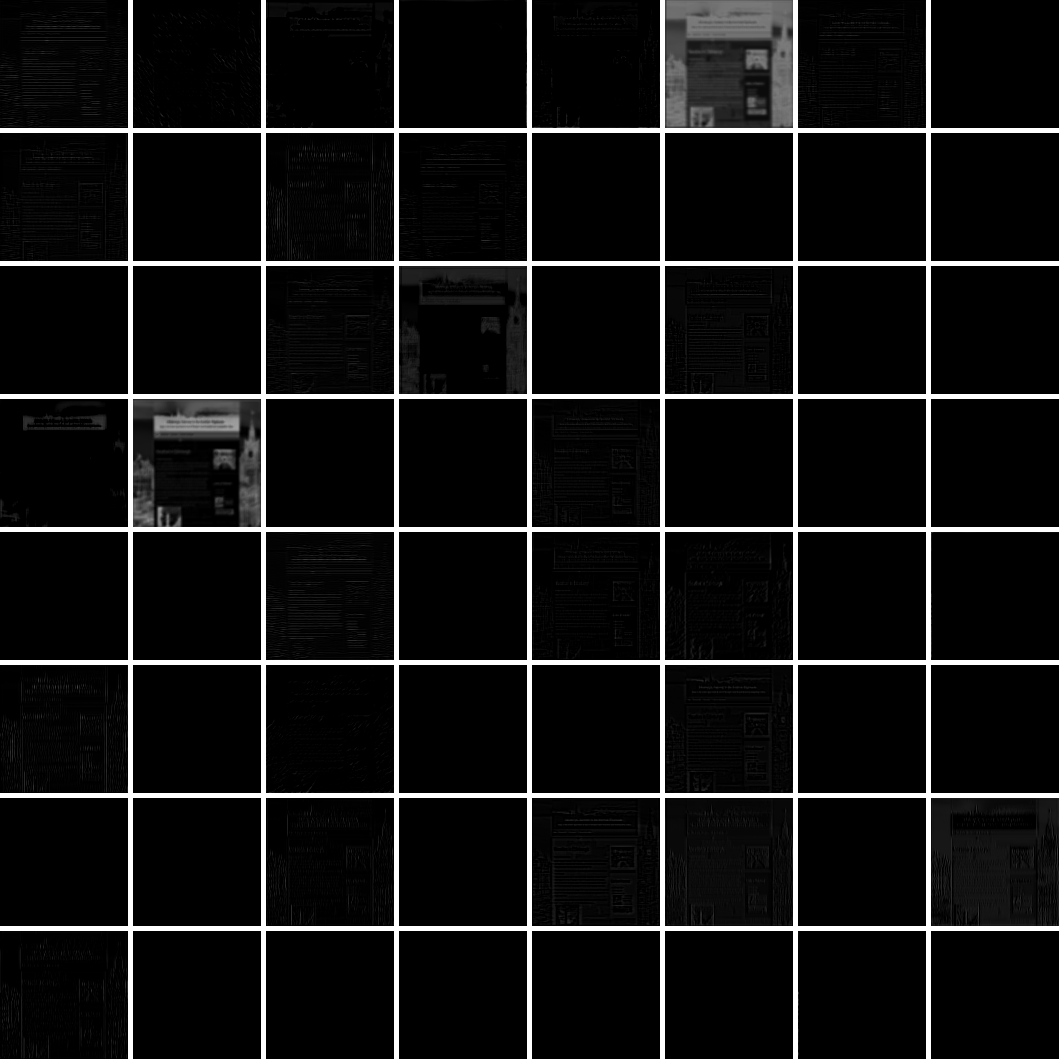
\includegraphics[width=0.6\columnwidth]{progettazione/feature_maps_layer_conv_2.png} 
  \caption{Feature map estratte dal secondo strato convoluzionale}
  \label{fig:conv-2}
\end{figure}

\begin{figure}[!htbp] 
  \centering 
  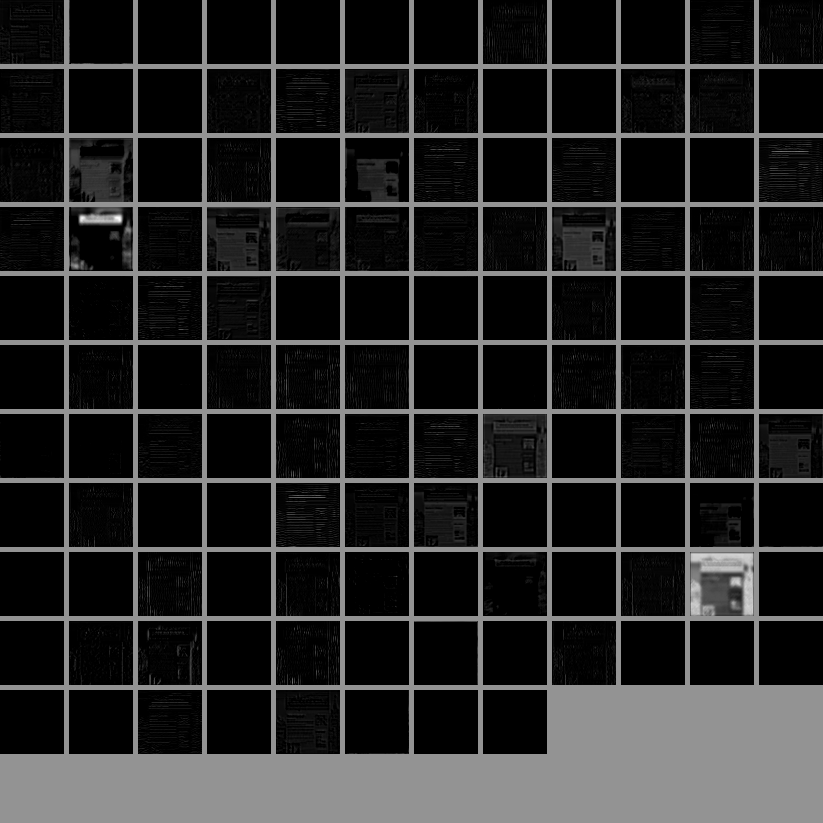
\includegraphics[width=0.6\columnwidth]{progettazione/feature_maps_layer_conv_3.png} 
  \caption{Feature map estratte dal terzo strato convoluzionale}
  \label{fig:conv-3}
\end{figure}

\newpage
Tramite l'utilizzo delle feature estratte dal bottleneck è possibile effettuare un clustering (Fig.~\ref{fig:cluster-conv})


\begin{figure}[!htbp] 
  \centering 
  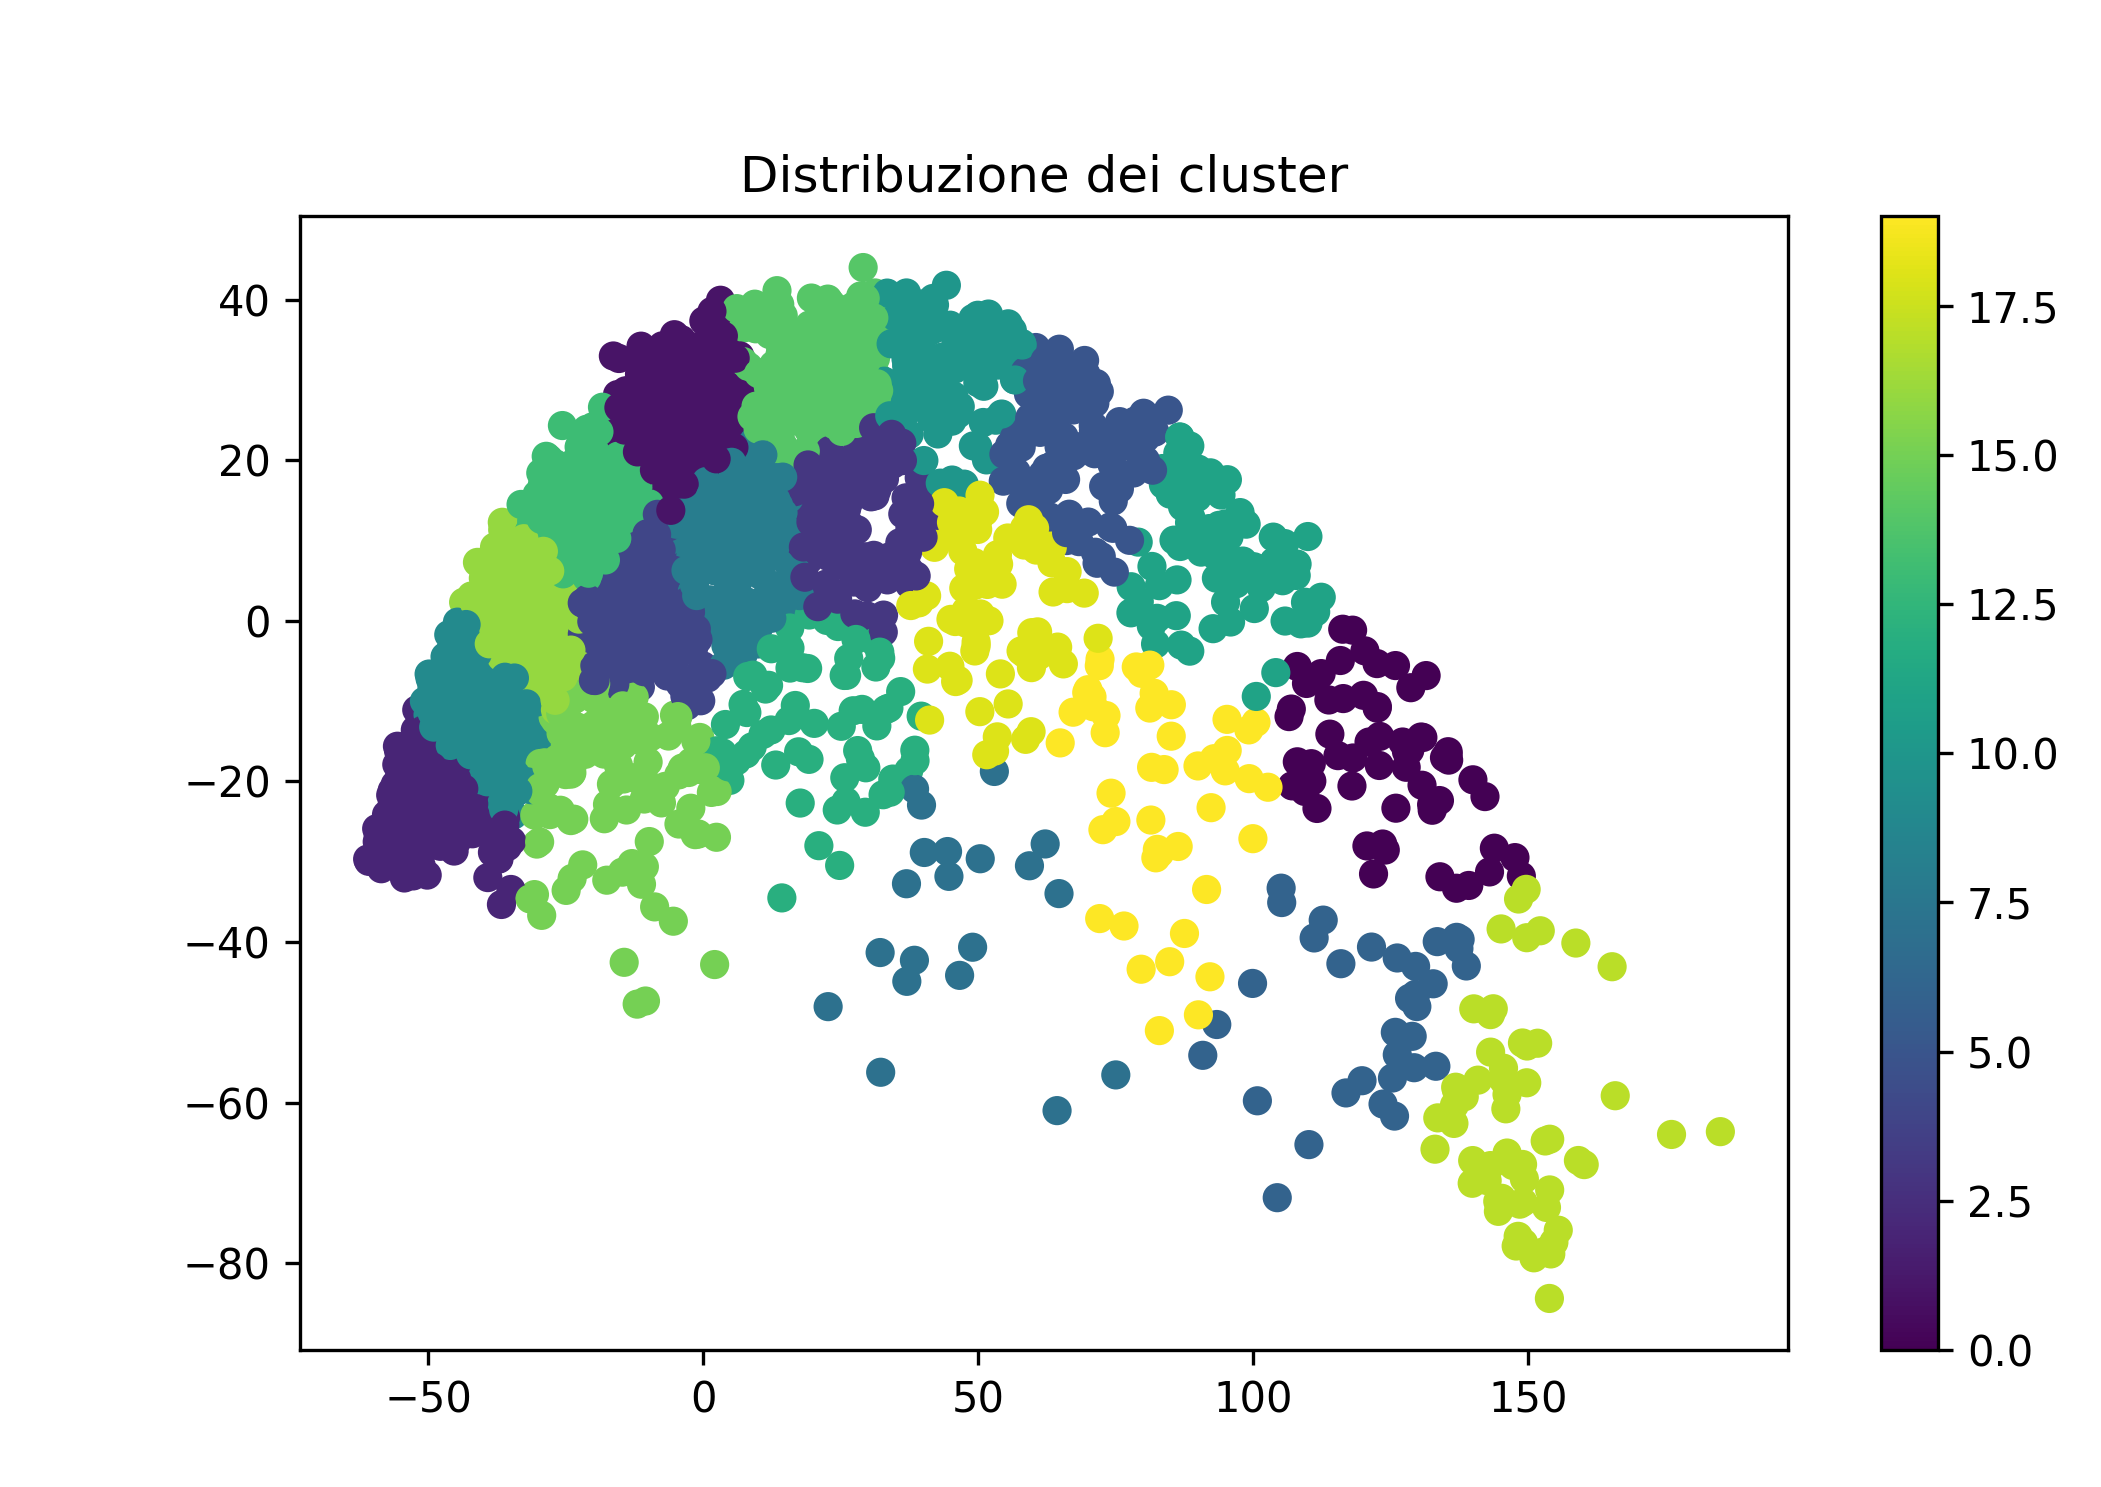
\includegraphics[width=0.7\columnwidth]{progettazione/Clusters_conv.png} 
  \caption{Clustering effettuato utilizzando le feature estratte dall'autoencoder convoluzionale; 20 clusters e 3000 immagini}
  \label{fig:cluster-conv}
\end{figure}

\newpage

\subsection{Modelli pre-addestrati}
L'utilizzo di un modello pre-addestrato consente di evitare la fase di addestramento e la complessa ingegnerizzazione di una rete neurale, per questo motivo l'utilizzo degli autoencoder è stato scartato.
Il modello consigliato dal tutor è ResNet50, la scelta viene avvalorata dalle motivazioni riportate nell'articolo\footcite{site:why-resnet}:
\begin{itemize}
  \item Facillità di addestramento.
  \item Bilanciamento tra performance ed efficienza rispetto ad altri modelli della stessa famiglia.
  \item Risultati simili o migliori utilizzando meno risorse rispetto alla famiglia VGGNet. 
\end{itemize}

\section{Clustering}
\subsection{Preparazione delle immagini}
In seguito alla cattura le immagini vengono lette dal database e convertite in un formato utilizzabile dagli algoritmi di machine learning (Fig.~\ref{fig:schema-resize}).
Per velocizzare le operazioni in fase di addestramento tutte le immagini vengono scaricate dal database e convertite in formato PNG, poiché le librerie utilizzate necessitano di dati raster per funzionare, successivamente le immagini salvate nella memoria del PC vengono processate in maniera tale da essere adatte all'utilizzo da parte di ResNet50.
In questo caso le dimensioni dei tensori richieste specificatamente dal modello (Fig.~\ref{fig:schema-tensore}) sono le seguenti (224*224*3):
\begin{itemize}
  \item Altezza dell'immagine
  \item Larghezza dell'immagine 
  \item Numero di canali (Red Green Blue)
\end{itemize}
Per rientrare nel formato richiesto le immagini subiscono un processo di scaling che ne riduce la dimensionalità lasciando il contenuto invariato.
Tale operazione è stata preferita al cropping perché utilizzandolo andrebbero a perdersi caratteristiche specifiche; ad esempio i margini bianchi ai lati del sito sono spesso segnale di un design un po'antiquato e migliorabile,  
la rimozione dei margini potrebbe compromettere il clustering impedendo la creazione di un cluster contenente pagine di quel tipo.
Inoltre ogni cella contiene valori compresi tra 0 e 255, per facilitare le operazioni tali valori vengono divisi per 255 e normalizzati in un intervallo compreso tra 0 e 1.

\begin{figure}[!h] 
  \centering 
  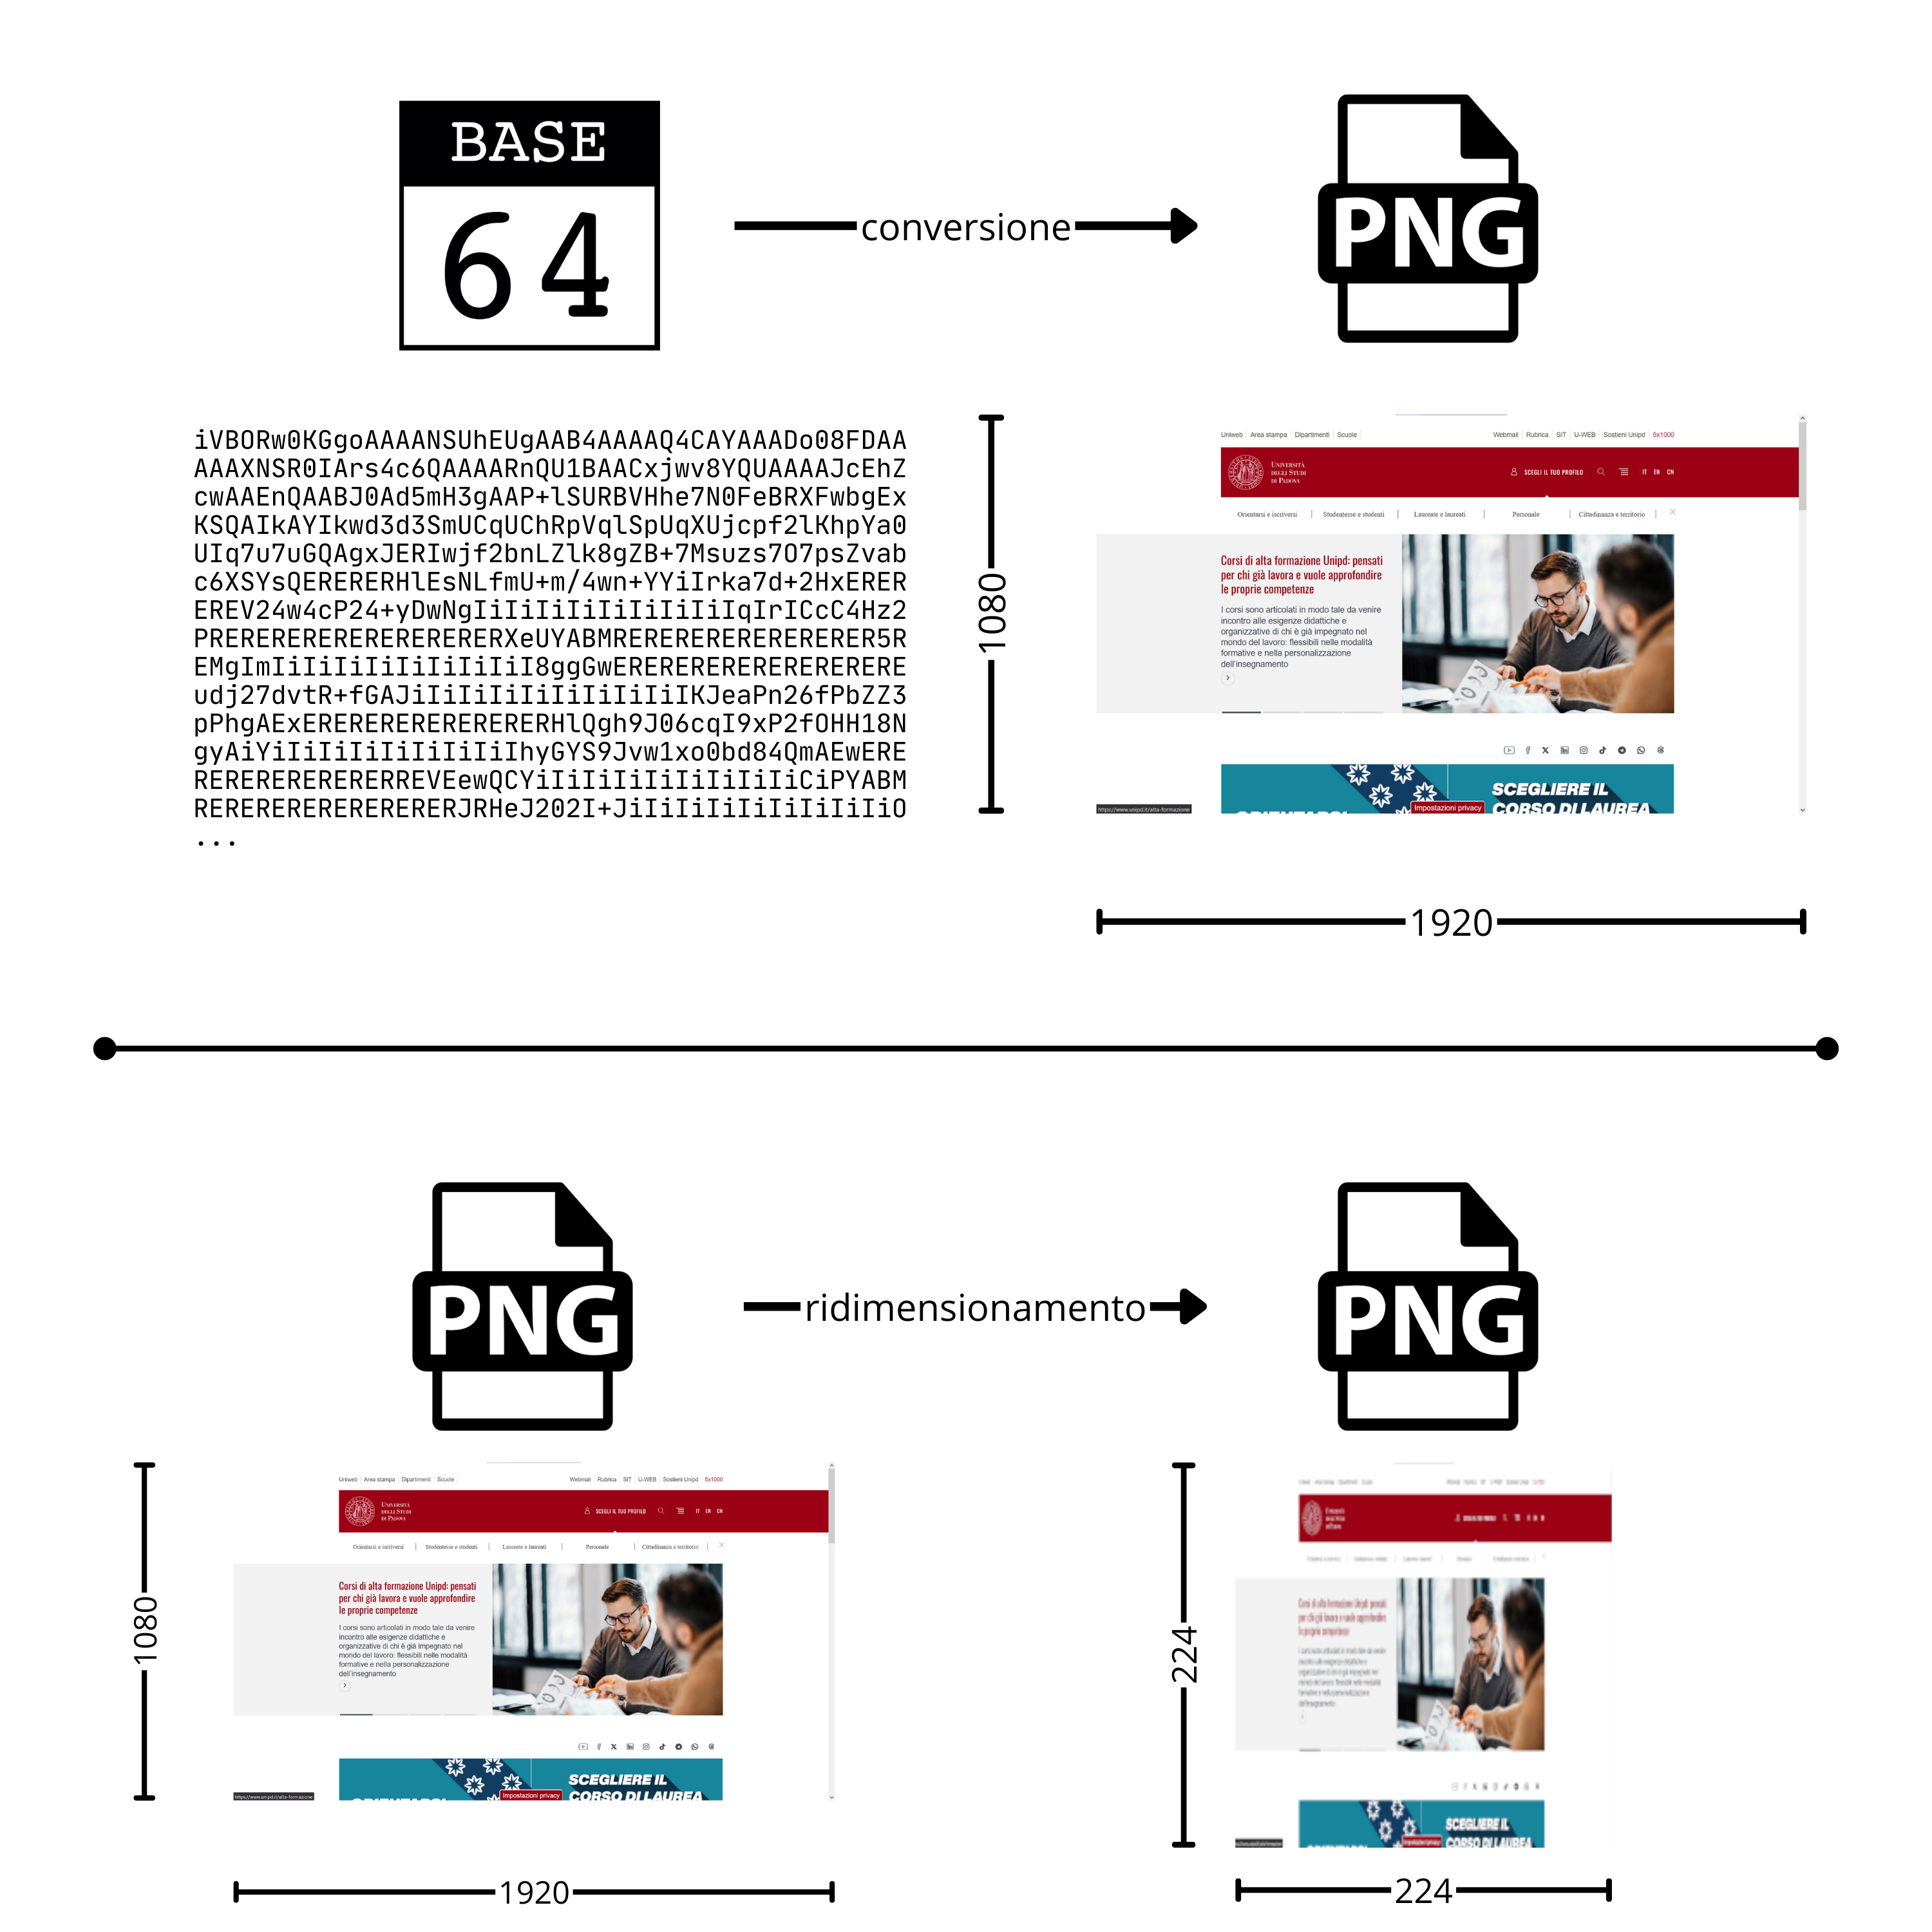
\includegraphics[width=0.7\columnwidth]{progettazione/schema-resize.png} 
  \caption{Conversione e ridimensionamento}
  \label{fig:schema-resize}
\end{figure}

\begin{figure}[!h] 
  \centering 
  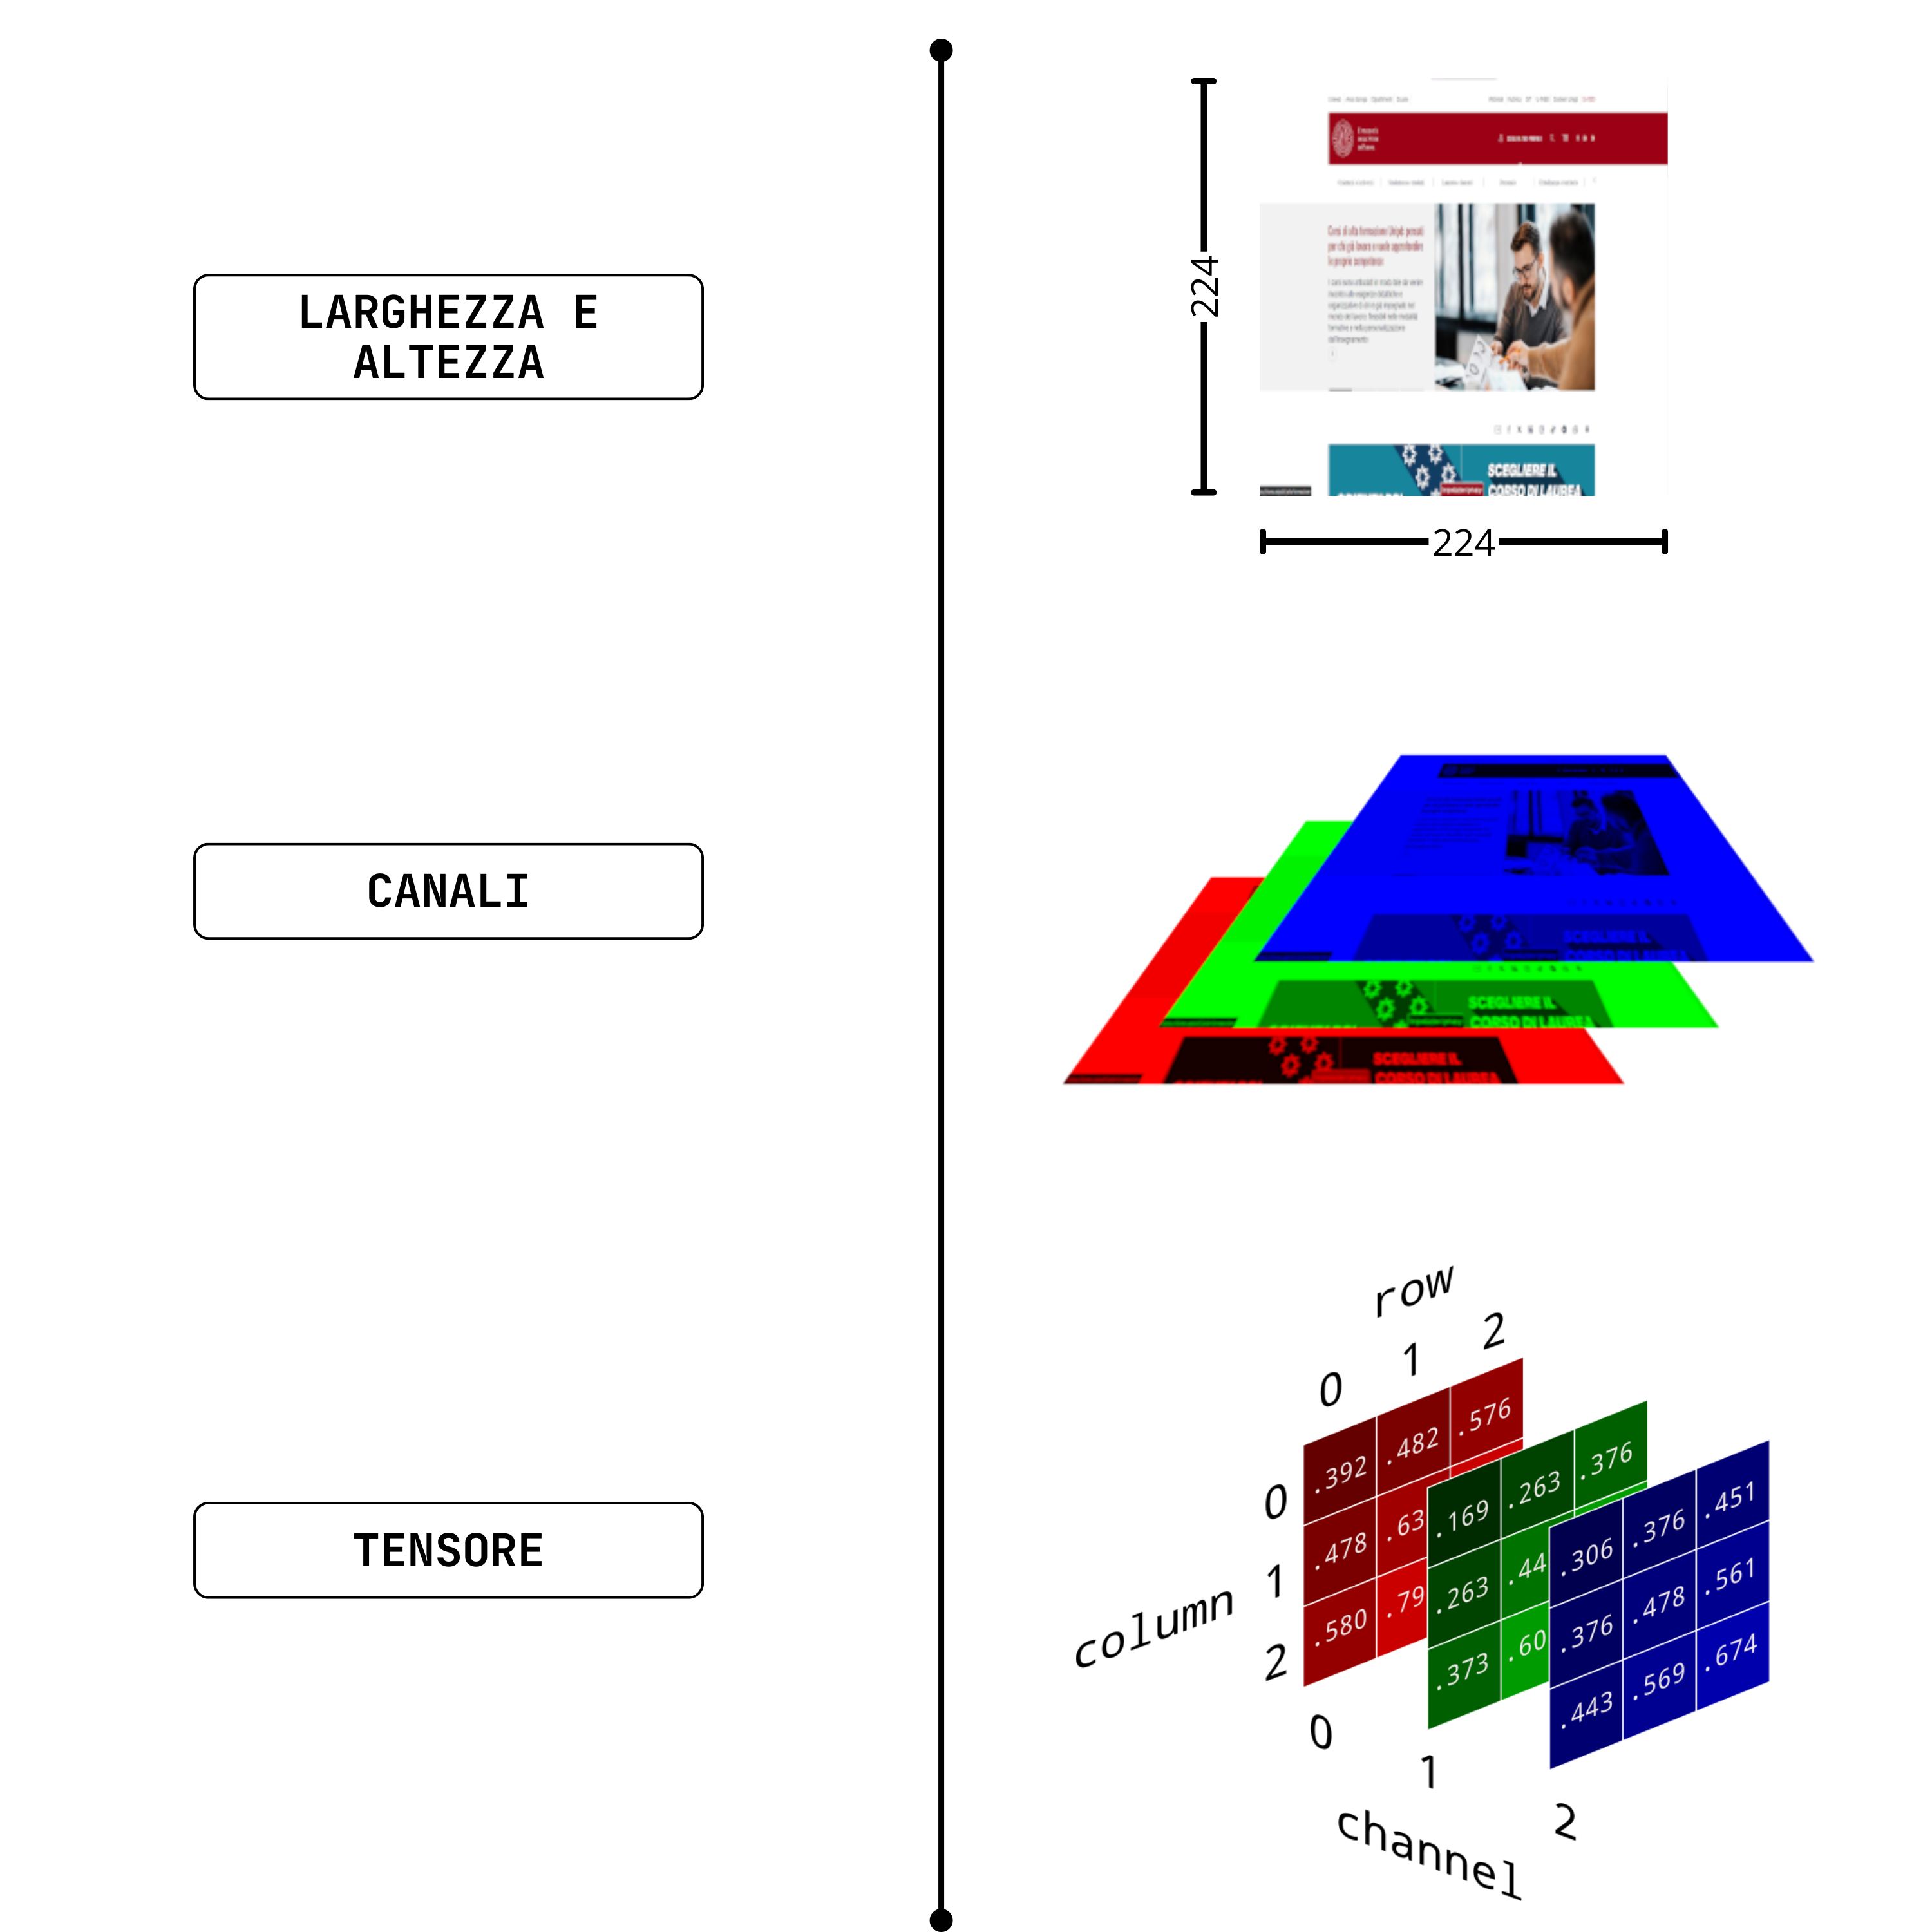
\includegraphics[width=0.5\columnwidth]{progettazione/schema-tensore.png} 
  \caption{Struttura del tensore}
  \label{fig:schema-tensore}
\end{figure}

\newpage


\subsection{Estrazione delle feature}
Per ottenere un dato utilizzabile in modo efficace dall'algoritmo di clustering è necessario modificare ulteriormente le immagini riducendole a un set di feature (Fig.~\ref{fig:featuremaps}).
Per adempire a questo compito viene utilizzato un CNN Convolutional Neural Network pre-addestrato chiamato ResNet50 (Fig.~\ref{fig:schema-resnet}).
Il modello viene caricato senza i top layer, ossia gli strati densi addetti alla classificazione, per sfruttare esclusivamente la sua abilità di riduzione in feature.

\begin{figure}[!h] 
  \centering 
  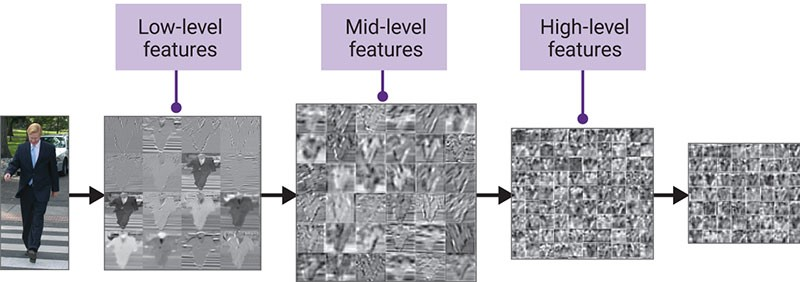
\includegraphics[width=0.7\columnwidth]{progettazione/esempio-featuremaps.png} 
  \caption{Esempio di featuremaps}
  \label{fig:featuremaps}
\end{figure}

\begin{figure}[!h] 
  \centering 
  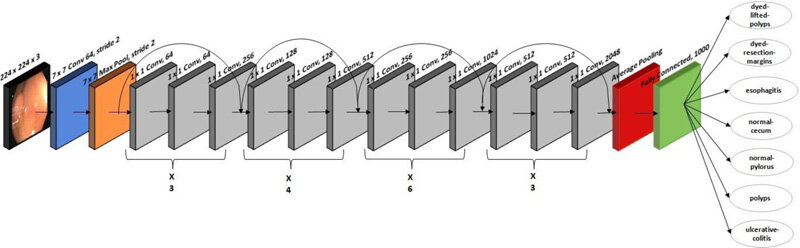
\includegraphics[width=0.9\columnwidth]{progettazione/schema-ResNet.png} 
  \caption{Struttura di ResNet50}
  \label{fig:schema-resnet}
\end{figure}



\subsection{Applicazione del clustering}
Le feature estratte dai layer convoluzionali vengono ridotte a uno stato bidimensionale sfruttando l'analisi dei componenti principali, in questa maniera è possibile visualizzare i risultati del clustering su un grafico cartesiano, ridurre i tempi di calcolo e aumentare l'accuratezza delle predizioni; ma al costo di una ovvia perdita di informazioni.
Successivamente viene applicato l'algoritmo dei K-means per l'effettiva suddivisione del dataset in clusters (Fig.~\ref{fig:clusters-resnet}).
Le immagini vengono inserite, in base al cluster a loro assegnato, nelle rispettive cartelle di appartenenza.
Questa operazione viene svolta per semplificare lo step successivo in cui lo sviluppatore deve preparare manualmente il dataset per l'addestramento supervisionato.

\begin{figure}[!h] 
  \centering 
  \includegraphics[width=0.7\columnwidth]{progettazione/Clusters-resnet.png} 
  \caption{Clustering effettuato utilizzando ResNet50; 20 clusters e 3000 immagini}
  \label{fig:clusters-resnet}
\end{figure}


%come modello finale è stato scelto resnet 50 poichè più rapido da utilizzare, infatti non necessita di addestramento 

\newpage

\section{Valutazione}

\subsection{Preparazione del dataset}
Il programmatore visiona i clusters ottenuti precedentemente e verifica quali possono appartenere alle categorie "siti migliorabili" e "siti ottimi"; prepara due cartelle corrispondenti alle categorie e inserisce le immagini che reputa appartenere a ciascun dominio.
Lo script prepara il dataset (Fig.~\ref{fig:struttura-dataset}) secondo la logica seguente:
\begin{itemize}
  \item Training, il 70\% delle immagini viene utilizzato per l'addestramento effettivo.
  \item Validation, il 15\% delle immagini viene utilizzato per ottimizzare i parametri del modello.
  \item Test, il 15\% delle immagini serve per valutare l'output del modello
\end{itemize}

\begin{figure}[!h] 
  \centering 
  \includegraphics[width=0.35\columnwidth]{progettazione/struttura-dataset.png} 
  \caption{Struttura del dataset}
  \label{fig:struttura-dataset}
\end{figure}

\subsection{Addestramento del modello}
Viene caricato il modello pre-addestrato ResNet50 escludendo i top-layer, congelando i pesi e aggiungendo degli strati personalizzati per la classificazione.
Gli strati di classificazione sono successivamente addestrati utilizzando come input le feature ricavate dai layer convoluzionali congelati di ResNet50. 

\subsection{Fine-tuning del modello}
I layer convoluzionali vengono sbloccati e il modello viene addestrato nuovamente nella sua interezza utilizzando un learning rate ridotto in maniera tale da non modificare completamente i pesi del modello pre-addestrato.
Il modello viene salvato e riutilizzato ogniqualvolta sia necessario.

\subsection{Valutazione delle immagini}
Le immagini presenti nel database vengono classificate dal modello e le valutazioni in centesimi vengono restituite.

\section{Invio e-mail}
Le valutazioni vengono lette dal database e tramite Laravel si procede all'invio di mail personalizzate alle aziende che dispongono di siti web che potrebbero essere ancora migliorati.

\section{Database}
Il database di SalesCRM contiene molte tabelle ma in questa sezione vengono descritte solo quelle utilizzate dal workflow.

\subsection{Domains}
Questa tabella contiene tutte i siti web (Fig.~\ref{fig:schema-domains}) delle aziende collezionate dal web-scraper e le informazioni a essi correlati.


\begin{figure}[!h] 
  \centering 
  \includegraphics[width=0.9\columnwidth]{progettazione/schema-domains.png} 
  \caption{Schema della tabella Domains}
  \label{fig:schema-domains}
\end{figure}


\subsection{Pages}
Contiene i link a tutte le pagine (Fig.~\ref{fig:schema-pages}) di ciascun dominio.

\begin{figure}[!h] 
  \centering 
  \includegraphics[width=0.9\columnwidth]{progettazione/schema-pages.png} 
  \caption{Schema della tabella Pages}
  \label{fig:schema-pages}
\end{figure}

    \chapter{Conclusioni}
\label{cap:conclusioni}

\section{Consuntivo finale}

\section{Raggiungimento degli obiettivi}

\section{Conoscenze acquisite}

\section{Valutazione personale}


    \backmatter
    \printglossary[type=\acronymtype, title=Acronimi e abbreviazioni, toctitle=Acronimi e abbreviazioni]
    \printglossary[type=main, title=Glossario, toctitle=Glossario]

    \cleardoublepage
\chapter{Bibliografia}

\nocite{*}

% Print book bibliography
\printbibliography[heading=subbibliography,title={Riferimenti bibliografici},type=book]

% Print site bibliography
\printbibliography[heading=subbibliography,title={Siti web consultati},type=online]

\end{document}
